%\RequirePackage{kvoptions-patch}
\documentclass[14pt, a4paper, twoside, bibliography=totoc, headsepline, cleardoublepage=empty, parskip=half, draft=false]{scrbook}
\DeclareUnicodeCharacter{2080}{$_{0}$}

\let\ifdeutsch\iffalse
\let\ifenglish\iftrue

% !TeX encoding = utf8
% -*- coding:utf-8 mod:LaTeX -*-

% EN: This file includes basic packages and sets options. The order of package
%     loading is important

% DE: In dieser Datei werden zuerst die benoetigten Pakete eingebunden und
%     danach diverse Optionen gesetzt. Achtung Reihenfolge ist entscheidend!


% EN: Styleguide:
% - English comments are prefixed with "EN", German comments are prefixed with "DE"
% - Prefixed headings define the language for the subsequent paragraphs
% - It is tried to organize packages in blocks. Bocks are separated by two empty lines.

% DE: Styleguide:
%
% Ein sehr kleiner Styleguide. Packages werden in Blöcken organisiert.
% Zwischen zwei Blöcken sind 2 Leerzeilen!


\RequirePackage{ifluatex}
\ifluatex
  % do not load anything
\else
  \ifdeutsch
    \RequirePackage[ngerman=ngerman-x-latest]{hyphsubst}
  \fi
\fi



% EN: Enable copy and paste of text from the PDF
%     Only required for pdflatex. It "just works" in the case of lualatex.
%     mmap enables mathematical symbols, but does not work with the newtx font set
%     See: https://tex.stackexchange.com/a/64457/9075
%     Other solutions outlined at http://goemonx.blogspot.de/2012/01/pdflatex-ligaturen-und-copynpaste.html and http://tex.stackexchange.com/questions/4397/make-ligatures-in-linux-libertine-copyable-and-searchable
%     Trouble shooting outlined at https://tex.stackexchange.com/a/100618/9075

\ifluatex
\else
  \usepackage{cmap}
\fi


% EN: File encoding
% DE: Codierung
%     Wir sind im 21 Jahrhundert, utf-8 löst so viele Probleme.
%
% Mit UTF-8 funktionieren folgende Pakete nicht mehr. Bitte beachten!
%   * fancyvrb mit §
%   * easylist -> http://www.ctan.org/tex-archive/macros/latex/contrib/easylist/
\ifluatex
  % EN: See https://tex.stackexchange.com/a/158517/9075
  %     Not required, because of usage of fontspec package
  %\usepackage[utf8]{luainputenc}
\else
  \usepackage[utf8]{inputenc}
\fi


% DE: Parallelbetrieb tex4ht und pdflatex
\makeatletter
\@ifpackageloaded{tex4ht}{
  \def\iftex4ht{\iftrue}
}{
  \def\iftex4ht{\iffalse}
}
\makeatother


% EN: Mathematics
% DE: Mathematik
%
% DE: Viele Mathematik-Sachen. Siehe https://texdoc.net/pkg/amsmath
%
% EN: Options must be passed this way, otherwise it does not work with glossaries
% DE: fleqn (=Gleichungen linksbündig platzieren) funktioniert nicht direkt. Es muss noch ein Patch gemacht werden:
\PassOptionsToPackage{fleqn,leqno}{amsmath}
%
% DE: amsmath Muss nicht mehr geladen werden, da es von newtxmath automatisch geladen wird
% \usepackage{amsmath}


%% EN: Fonts
%% DE: Schriften
%%
%% !!! If you change the font, be sure that words such as "workflow" can
%% !!! still be copied from the PDF. If this is not the case, you have
%% !!! to use glyphtounicode. See comment at cmap package


% EN: Times Roman for all text
\ifluatex
  % source: Second proposed fix from the following answer: https://tex.stackexchange.com/a/394137
  \usepackage[no-math]{fontspec}
  \setmainfont{TeXGyreTermes-Regular}[
       BoldFont       = TeXGyreTermes-Bold ,
       ItalicFont     = TeXGyreTermes-Italic ,
       BoldItalicFont = TeXGyreTermes-BoldItalic,
       NFSSFamily     = ntxtlf]
  \setsansfont{TeX Gyre Heros Regular}[
       Scale=.9,
       BoldFont       = TeX Gyre Heros Bold,
       ItalicFont     = TeX Gyre Heros Italic,
       BoldItalicFont = TeX Gyre Heros BoldItalic]
  \setmonofont[StylisticSet={1,3},Scale=.9]{inconsolata}
  \RequirePackage{newtxmath}
\else
  \RequirePackage{newtxtext}
  \RequirePackage{newtxmath}
  % EN: looks good with times, but no equivalent for lualatex found,
  %     therefore replaced with inconsolata
  %\RequirePackage[zerostyle=b,scaled=.9]{newtxtt}
  \RequirePackage[varl,scaled=.9]{inconsolata}
\fi


% EN: backticks (`) are rendered as such in verbatim environments.
%     See following links for details:
%     - https://tex.stackexchange.com/a/341057/9075
%     - https://tex.stackexchange.com/a/47451/9075
%     - https://tex.stackexchange.com/a/166791/9075
\usepackage{upquote}
\usepackage{tabularx}  % Add this line

% DE: Symbole
%
%\usepackage[geometry]{ifsym} % \BigSquare
%\usepackage{mathabx}
%\usepackage{stmaryrd} %fuer \ovee, \owedge, \otimes
%\usepackage{marvosym} %fuer \Writinghand %patched to not redefine \Rightarrow
%\usepackage{mathrsfs} %mittels \mathscr{} schoenen geschwungenen Buchstaben erzeugen
%\usepackage{calrsfs} %\mathcal{} ein bisserl dickeren buchstaben erzeugen - sieht net so gut aus.
%durch mathpazo ist das schon definiert

%
%\usepackage{amssymb}

% EN: For \texttrademark{}
\usepackage{textcomp}

% EN: name-clashes von marvosym und mathabx vermeiden:
\def\delsym#1{%
  %  \expandafter\let\expandafter\origsym\expandafter=\csname#1\endcsname
  %  \expandafter\let\csname orig#1\endcsname=\origsym
  \expandafter\let\csname#1\endcsname=\relax
}

%\usepackage{pifont}
%\usepackage{bbding}
%\delsym{Asterisk}
%\delsym{Sun}\delsym{Mercury}\delsym{Venus}\delsym{Earth}\delsym{Mars}
%\delsym{Jupiter}\delsym{Saturn}\delsym{Uranus}\delsym{Neptune}
%\delsym{Pluto}\delsym{Aries}\delsym{Taurus}\delsym{Gemini}
%\delsym{Rightarrow}
%\usepackage{mathabx} - Ueberschreibt leider zu viel - und die \le-Zeichen usw. sehen nicht gut aus!


% EN: Modern font encoding
%     Has to be loaded AFTER any font packages. See https://tex.stackexchange.com/a/2869/9075.
\ifluatex
\else
  \usepackage[T1]{fontenc}
\fi
%


% EN: Character protrusion and font expansion. See http://www.ctan.org/tex-archive/macros/latex/contrib/microtype/
% DE: Optischer Randausgleich und Grauwertkorrektur

\usepackage[
  babel=true, % EN: Enable language-specific kerning. Take language-settings from the languge of the current document (see Section 6 of microtype.pdf)
  expansion=alltext,
  protrusion=alltext-nott, % EN: Ensure that at listings, there is no change at the margin of the listing
  final % EN: Always enable microtype, even if in draft mode. This helps finding bad boxes quickly.
        %     In the standard configuration, this template is always in the final mode, so this option only makes a difference if "pros" use the draft mode
]{microtype}


% EN: \texttt{test -- test} keeps the "--" as "--" (and does not convert it to an en dash)
\DisableLigatures{encoding = T1, family = tt* }

% DE: fuer microtype
% DE: tracking=true muss als Parameter des microtype-packages mitgegeben werden
% DE: Deaktiviert, da dies bei Algorithmen seltsam aussieht

%\DeclareMicrotypeSet*[tracking]{my}{ font = */*/*/sc/* }%
%\SetTracking{ encoding = *, shape = sc }{ 45 }
% DE: Hier wird festgelegt,
%     dass alle Passagen in Kapitälchen automatisch leicht
%     gesperrt werden.
%     Quelle: http://homepage.ruhr-uni-bochum.de/Georg.Verweyen/pakete.html
%    Deaktiviert, da sonst "BPEL", "BPMN" usw. wirklich komisch aussehen.
%     Macht wohl nur bei geisteswissenschaftlichen Arbeiten Sinn.


% EN: amsmath teaks


% EN: Fixes bugs in AMS math
%     Corrently conflicts with unicode-math
% \usepackage{mathtools}

%\numberwithin{equation}{section}
%\renewcommand{\theequation}{\thesection.\Roman{equation}}

% EN: work-around ams-math problem with align and 9 -> 10. Does not work with glossaries, No visual changes.
%\addtolength\mathindent{1em}


% EN: For theorems, replacement for amsthm
%\usepackage[amsmath,hyperref]{ntheorem}
%\theorempreskipamount 2ex plus1ex minus0.5ex
%\theorempostskipamount 2ex plus1ex minus0.5ex
%\theoremstyle{break}
%\newtheorem{definition}{Definition}[section]


% CTAN: https://ctan.org/pkg/lccaps
% Doc: http://texdoc.net/pkg/lccaps
%
% Required for DE/EN \initialism
\usepackage{lccaps}


% EN: Defintion of colors. Argument "hyperref" is not used as we do not want to change border colors of links: Links are not colored anymore.
% DE: Farbdefinitionen
\usepackage[dvipsnames]{xcolor}


% EN: Required for custom acronyms/glossaries style.
%     Left aligned Columns in tables with fixed width.
%     See http://tex.stackexchange.com/questions/91566/syntax-similar-to-centering-for-right-and-left
\usepackage{ragged2e}


% DE: Wichtig, ansonsten erscheint "No room for a new \write"
%\usepackage{scrwfile}


% EN: Support for language-specific hyphenation
% DE: Neue deutsche Rechtschreibung und Literatur statt "Literature"
%     Die folgende Einstellung ist der Nachfolger von ngerman.sty
\ifdeutsch
  % DE: letzte Sprache ist default, Einbindung von "american" ermöglicht \begin{otherlanguage}{amercian}...\end{otherlanguage} oder \foreignlanguage{american}{Text in American}
  %     Siehe auch http://tex.stackexchange.com/a/50638/9075
  \usepackage[american,main=ngerman]{babel}
  % Ein "abstract" ist eine "Kurzfassung", keine "Zusammenfassung"
  \addto\captionsngerman{%
    \renewcommand\abstractname{Kurzfassung}%
  }
  \ifluatex
    % EN: conditionally disable ligatures. See https://github.com/latextemplates/scientific-thesis-template/issues/54
    %     for a discussion
    \usepackage[ngerman]{selnolig}
  \fi
\else
  % EN: Set English as language and allow to write hyphenated"=words
  %     `american`, `english` and `USenglish` are synonyms for babel package (according to https://tex.stackexchange.com/questions/12775/babel-english-american-usenglish).
  %      "english" has to go last to set it as default language
  \usepackage[english]{babel}
  % EN: Hint by http://tex.stackexchange.com/a/321066/9075 -> enable "= as dashes
  \addto\extrasenglish{\languageshorthands{ngerman}\useshorthands{"}}
  \ifluatex
    % EN: conditionally disable ligatures. See https://github.com/latextemplates/scientific-thesis-template/issues/54
    %     for a discussion
    \usepackage[english]{selnolig}
  \fi
\fi
%


% EN: For easy quotations: \enquote{text}
%     This package is very smart when nesting is applied, otherwise textcmds (see below) provides a shorter command
%     Note that this package results in a warning when it is loaded before minted (actually fvextra).
% DE: Anführungszeichen
%     Zitate in \enquote{...} setzen, dann werden automatisch die richtigen Anführungszeichen verwendet.
%     Dieses package erzeugt eine Warnung, wenn es vor minted (genauer fvextra) geladen wird.
\usepackage{csquotes}


% EN: For even easier quotations: \qq{text}.
%     Is not smart in the case of nesting, but good enough for the most cases
%\usepackage{textcmds}
%\ifdeutsch
%  % EN: German quotes are different. So do not use the English quotes, but the ones provided by the csquotes package.
%  \renewcommand{\qq}[1]{\enquote{#1}}
%\fi


% EN: extended enumarations
% DE: erweitertes Enumerate
\usepackage{paralist}


% DE: Gestaltung der Kopf- und Fußteilen

\usepackage[automark]{scrlayer-scrpage}

\automark[section]{chapter}
\setkomafont{pageheadfoot}{\normalfont\sffamily}
\setkomafont{pagenumber}{\normalfont\sffamily}

% DE: funktioniert nicht: Alle Linien sind hier weg
%\setheadsepline[.4pt]{.4pt}


% DE: Intelligentes Leerzeichen um hinter Abkürzungen die richtigen Abstände zu erhalten, auch leere.
%     Siehe commands.tex \gq{}
\usepackage{xspace}
% DE: Macht \xspace und \enquote kompatibel
\makeatletter
\xspaceaddexceptions{\grqq \grq \csq@qclose@i \} }
\makeatother


\newcommand{\eg}{e.\,g.,\ }
\newcommand{\ie}{i.\,e.,\ }


% EN: introduce \powerset - hint by http://matheplanet.com/matheplanet/nuke/html/viewtopic.php?topic=136492&post_id=997377
\DeclareFontFamily{U}{MnSymbolC}{}
\DeclareSymbolFont{MnSyC}{U}{MnSymbolC}{m}{n}
\DeclareFontShape{U}{MnSymbolC}{m}{n}{
  <-6>    MnSymbolC5
  <6-7>   MnSymbolC6
  <7-8>   MnSymbolC7
  <8-9>   MnSymbolC8
  <9-10>  MnSymbolC9
  <10-12> MnSymbolC10
  <12->   MnSymbolC12%
}{}
\DeclareMathSymbol{\powerset}{\mathord}{MnSyC}{180}


% EN: Package for the appendix
% DE: Anhang
\usepackage{appendix}
%[toc,page,title,header]
%


% EN: Graphics
% DE: Grafikeinbindungen
%
% EN: The parameter "pdftex" is not required
\usepackage{graphicx}
\graphicspath{{\getgraphicspath}}
\newcommand{\getgraphicspath}{graphics/}


% EN: Enables inclusion of SVG graphics - 1:1 approach
%    This is NOT the approach of https://ctan.org/pkg/svg-inkscape,
%     which allows text in SVG to be typeset using LaTeX
%     We just include the SVG as is.
\usepackage{epstopdf}
\epstopdfDeclareGraphicsRule{.svg}{pdf}{.pdf}{%
  inkscape -z -D --file=#1 --export-pdf=\OutputFile
}


% EN: Enables inclusion of SVG graphics - text-rendered-with-LaTeX-approach
%     This is the approach of https://ctan.org/pkg/svg-inkscape,
\newcommand{\executeiffilenewer}[3]{%
  \IfFileExists{#2}
  {
    %\message{file #2 exists}
    \ifnum\pdfstrcmp{\pdffilemoddate{#1}}%
      {\pdffilemoddate{#2}}>0%
      {\immediate\write18{#3}}
    \else
      {%\message{file up to date #2}
      }
    \fi%
  }{
    %\message{file #2 doesn't exist}
    %\message{argument: #3}
    %\immediate\write18{echo "test" > xoutput.txt}
    \immediate\write18{#3}
  }
}
\newcommand{\includesvg}[1]{%
  \executeiffilenewer{#1.svg}{#1.pdf}%
  {
    inkscape -z -D --file=\getgraphicspath#1.svg %
    --export-pdf=\getgraphicspath#1.pdf --export-latex}%
  \input{\getgraphicspath#1.pdf_tex}%
}


% EN: Enable typesetting values with SI units.
%\ifdeutsch
%  \usepackage[mode=text,group-four-digits]{siunitx}
%  \sisetup{locale=DE}
%\else
%  \usepackage[mode=text,group-four-digits,group-separator={,}]{siunitx}
%  \sisetup{locale=US}
%\fi


% EN: Extensions for tables
% DE: Tabellenerweiterungen
\usepackage{array} %increases tex's buffer size and enables ``>'' in tablespecs
\usepackage{longtable}
\usepackage{dcolumn} %Aligning numbers by decimal points in table columns
\ifdeutsch
  \newcolumntype{d}[1]{D{.}{,}{#1}}
\else
  \newcolumntype{d}[1]{D{.}{.}{#1}}
\fi
\setlength{\extrarowheight}{1pt}


% DE: Eine Zelle, die sich über mehrere Zeilen erstreckt.
%     Siehe Beispieltabelle in Kapitel 2
\usepackage{multirow}


% DE: Fuer Tabellen mit Variablen Spaltenbreiten
%\usepackage{tabularx}
%\usepackage{tabulary}


% EN: Links behave as they should. Enables "\url{...}" for URL typesettings.
%     Allow URL breaks also at a hyphen, even though it might be confusing: Is the "-" part of the address or just a hyphen?
%     See https://tex.stackexchange.com/a/3034/9075.
% DE: Links verhalten sich so, wie sie sollen
%     Zeilenumbrüche bei URLs auch bei Bindestrichen erlauben, auch wenn es verwirrend sein könnte: Gehört der Bindestrich zur URL oder ist es ein Trennstrich?
%     Siehe https://tex.stackexchange.com/a/3034/9075.
\usepackage[hyphens]{url}
%
%  EN: When activated, use text font as url font, not the monospaced one.
%      For all options see https://tex.stackexchange.com/a/261435/9075.
% \urlstyle{same}
%
% EN: Hint by http://tex.stackexchange.com/a/10419/9075.
\makeatletter
\g@addto@macro{\UrlBreaks}{\UrlOrds}
\makeatother


% DE: Index über Begriffe, Abkürzungen
%\usepackage{makeidx} makeidx ist out -> http://xindy.sf.net verwenden


% DE: lustiger Hack fuer das Abkuerzungsverzeichnis
%     nach latex durchlauf folgendes ausfuehren
%     makeindex ausarbeitung.nlo -s nomencl.ist -o ausarbeitung.nls
%     danach nochmal latex
%\usepackage{nomencl}
%    \let\abk\nomenclature %Deutsche Ueberschrift setzen
%          \renewcommand{\nomname}{List of Abbreviations}
%        %Punkte zw. Abkuerzung und Erklaerung
%          \setlength{\nomlabelwidth}{.2\hsize}
%          \renewcommand{\nomlabel}[1]{#1 \dotfill}
%        %Zeilenabstaende verkleinern
%          \setlength{\nomitemsep}{-\parsep}
%    \makenomenclature


% EN: Logic for TeX - enables if-then-else in commands
% DE: Logik für TeX
%     FÜr if-then-else @ commands.tex
\usepackage{ifthen}


% EN: Code Listings
% DE: Listings
\usepackage{listings}
\lstset{language=XML,
  showstringspaces=false,
  extendedchars=true,
  basicstyle=\footnotesize\ttfamily,
  commentstyle=\slshape,
  % DE: Original: \rmfamily, damit werden die Strings im Quellcode hervorgehoben. Zusaetzlich evtl.: \scshape oder \rmfamily durch \ttfamily ersetzen. Dann sieht's aus, wie bei fancyvrb
  stringstyle=\ttfamily,
  breaklines=true,
  breakatwhitespace=true,
  % EN: alternative: fixed
  columns=flexible,
  numbers=left,
  numberstyle=\tiny,
  basewidth=.5em,
  xleftmargin=.5cm,
  % aboveskip=0mm, %DE: deaktivieren, falls man lstlistings direkt als floating object benutzt (\begin{lstlisting}[float,...])
  % belowskip=0mm, %DE: deaktivieren, falls man lstlistings direkt als floating object benutzt (\begin{lstlisting}[float,...])
  captionpos=b
}

\ifluatex
\else
  % EN: Enable UTF-8 support - see https://tex.stackexchange.com/q/419327/9075
  \usepackage{listingsutf8}
  \lstset{inputencoding=utf8/latin1}
\fi

\ifdeutsch
  \renewcommand{\lstlistlistingname}{Verzeichnis der Listings}
\fi


% EN: Alternative to listings could be fancyvrb. Can be used together.
% DE: Alternative zu Listings ist fancyvrb. Kann auch beides gleichzeitig benutzt werden.
\usepackage{fancyvrb}
%
% EN: Font size for the normal text
% DE: Groesse fuer den Fliesstext. Falls deaktiviert: \normalsize
%\fvset{fontsize=\small}
%
% DE: Somit kann im Text ganz einfach §verbatim§ text gesetzt werden.
%     Disabled, because UTF-8 does not work any more and lualatex causes issues
%\DefineShortVerb{\§}
%
% EN: Shrink font size of listings
\RecustomVerbatimEnvironment{Verbatim}{Verbatim}{fontsize=\footnotesize}
\RecustomVerbatimCommand{\VerbatimInput}{VerbatimInput}{fontsize=\footnotesize}
%
% EN: Hack for fancyvrb based on http://newsgroups.derkeiler.com/Archive/Comp/comp.text.tex/2008-12/msg00075.html
%     Change of the solution: \Vref somehow collidated with cleveref/varioref as the output of \Vref{} was "Abschnitt 4.3 auf Seite 85"; therefore changed to \myVref -- so completely removed
%     See https://tex.stackexchange.com/q/132420/9075 for more information.
\newcommand{\Vlabel}[1]{\label[line]{#1}\hypertarget{#1}{}}
\newcommand{\lref}[1]{\hyperlink{#1}{\FancyVerbLineautorefname~\ref*{#1}}}


% EN: Tunings of captions for floats, listings, ...
% DE: Bildunterschriften bei floats genauso formatieren wie bei Listings
%     Anpassung wird unten bei den newfloat-Deklarationen vorgenommen
%     https://www.ctan.org/pkg/caption2 is superseeded by this package.
\usepackage{caption}


% EN: Provides rotating figures, where the PDF page is also turned
% DE: Ermoeglicht es, Abbildungen um 90 Grad zu drehen
%     Alternatives Paket: rotating Allerdings wird hier nur das Bild gedreht, während bei lscape auch die PDF-Seite gedreht wird.
%     Das Paket lscape dreht die Seite auch nicht
\usepackage{pdflscape}


% EN: Required for proper environments of fancyvrb and lstlistings
%    There is also the newfloat pacakge (recommended by minted), but we currently have no expericene with that
% DE: Wird für fancyvrb und für lstlistings verwendet
\usepackage{float}
%
% EN: Alternative to float package
%\usepackage{floatrow}
% DE: zustäzlich für den Paramter [H] = Floats WIRKLICH da wo sie deklariert wurden paltzieren - ganz ohne Kompromisse
%     floatrow ist der Nachfolger von float
%     Allerdings macht floatrow in manchen Konstellationen Probleme. Deshalb ist das Paket deaktiviert.
%
% EN: See http://www.tex.ac.uk/cgi-bin/texfaq2html?label=floats
% DE: floats IMMER nach einer Referenzierung platzieren
%\usepackage{flafter}


% EN: Put footnotes below floats
%     Source: https://tex.stackexchange.com/a/32993/9075
\usepackage{stfloats}
\fnbelowfloat


% EN: For nested figures
% DE: Fuer Abbildungen innerhalb von Abbildungen
%     Ersetzt die Pakete subfigure und subfig - siehe https://tex.stackexchange.com/a/13778/9075
\usepackage[hypcap=true]{subcaption}


% EN: Extended support for footnotes
% DE: Fußnoten
%
%\usepackage{dblfnote}  %Zweispaltige Fußnoten
%
% Keine hochgestellten Ziffern in der Fußnote (KOMA-Script-spezifisch):
%\deffootnote[1.5em]{0pt}{1em}{\makebox[1.5em][l]{\bfseries\thefootnotemark}}
%
% Abstand zwischen Fußnoten vergrößern:
%\setlength{\footnotesep}{.85\baselineskip}
%
% EN: Following command disables the separting line of the footnote
% DE: Folgendes Kommando deaktiviert die Trennlinie zur Fußnote
%\renewcommand{\footnoterule}{}
%
\addtolength{\skip\footins}{\baselineskip} % Abstand Text <-> Fußnote
%
% Fußnoten immer ganz unten auf einer \raggedbottom-Seite
% fnpos kommt aus dem yafoot package
\usepackage{fnpos}
\makeFNbelow
\makeFNbottom


% EN: Variable page heights
% DE: Variable Seitenhöhen zulassen
\raggedbottom


% EN: More beautiful tables if one uses \toprule, \midrule, \bottomrule
% DE: Noch schoenere Tabellen als mit booktabs mit http://www.zvisionwelt.de/downloads.html
\usepackage{booktabs}
%
%\usepackage[section]{placeins}


% EN: Graphs and Automata
%
% TODO: Since version 3.0 (2013-10-01), it supports pdflatex via the auto-pst-pdf package
%       Requires -shell-escape
%\usepackage{gastex}


%\usepackage{multicol}

% DE: kollidiert mit diplomarbeit.sty
%\usepackage{setspace}


% DE: biblatex statt bibtex
\usepackage[
  backend       = biber, %biber does not work with 64x versions alternative: bibtex8
  %minalphanames only works with biber backend
  sortcites     = true,
  bibstyle      = numeric,
  citestyle     = numeric,
  giveninits    = false,
  useprefix     = false, %"von, van, etc." will be printed, too. See below.
  minnames      = 1,
  minalphanames = 3,
  maxalphanames = 4,
  maxbibnames   = 99,
  maxcitenames  = 2,
  natbib        = true,
  eprint        = true,
  url           = true,
  doi           = true,
  isbn          = true,
  backref       = false]{biblatex}

% enable more breaks at URLs. See https://tex.stackexchange.com/a/134281.
\setcounter{biburllcpenalty}{7000}
\setcounter{biburlucpenalty}{8000}

\bibliography{bibliography}
%\addbibresource[datatype=bibtex]{bibliography.bib}

%Do not put "vd" in the label, but put it at "\citeauthor"
%Source: http://tex.stackexchange.com/a/30277/9075
\makeatletter
\AtBeginDocument{\toggletrue{blx@useprefix}}
\AtBeginBibliography{\togglefalse{blx@useprefix}}
\makeatother

%Thin spaces between initials
%http://tex.stackexchange.com/a/11083/9075
\renewrobustcmd*{\bibinitdelim}{\,}

%Keep first and last name together in the bibliography
%http://tex.stackexchange.com/a/196192/9075
\renewcommand*\bibnamedelimc{\addnbspace}
\renewcommand*\bibnamedelimd{\addnbspace}

%Replace last "and" by comma in bibliography
%See http://tex.stackexchange.com/a/41532/9075
\AtBeginBibliography{%
  \renewcommand*{\finalnamedelim}{\addcomma\space}%
}

\ifdeutsch
  \DefineBibliographyStrings{ngerman}{
    backrefpage  = {zitiert auf S\adddot},
    backrefpages = {zitiert auf S\adddot},
    andothers    = {et\ \addabbrvspace al\adddot},
    %Tipp von http://www.mrunix.de/forums/showthread.php?64665-biblatex-Kann-%DCberschrift-vom-Inhaltsverzeichnis-nicht-%E4ndern&p=293656&viewfull=1#post293656
    bibliography = {Literaturverzeichnis}
  }
\fi

% Note: This breaks Overleaf word count. Just use \citet
% EN: enable hyperlinked author names when using \citeauthor
%     source: http://tex.stackexchange.com/a/75916/9075
%\DeclareCiteCommand{\citeauthor}
%{\boolfalse{citetracker}%
%  \boolfalse{pagetracker}%
%  \usebibmacro{prenote}}
%{\ifciteindex
%  {\indexnames{labelname}}
%  {}%
%  \printtext[bibhyperref]{\printnames{labelname}}}
%{\multicitedelim}
%{\usebibmacro{postnote}}


% EN: natbib compatibility
%\newcommand{\citep}[1]{\cite{#1}}
%\newcommand{\citet}[1]{\citeauthor{#1} \cite{#1}}
% EN: Beginning of sentence - analogous to cleveref - important for names such as "zur Muehlen"
%\newcommand{\Citep}[1]{\cite{#1}}
%\newcommand{\Citet}[1]{\Citeauthor{#1} \cite{#1}}

% DE: Blindtext. Paket "blindtext" ist fortgeschritterner als "lipsum" und kann auch Mathematik im Text (http://texblog.org/2011/02/26/generating-dummy-textblindtext-with-latex-for-testing/)
%     kantlipsum (https://www.ctan.org/tex-archive/macros/latex/contrib/kantlipsum) ist auch ganz nett, aber eben auch keine Mathematik
%     Wird verwendet, um etwas Text zu erzeugen, um eine volle Seite wegen Layout zu sehen.
\usepackage[math]{blindtext}


% DE: Neue Pakete bitte VOR hyperref einbinden. Insbesondere bei Verwendung des
%     Pakets "index" wichtig, da sonst die Referenzierung nicht funktioniert.
%     Für die Indizierung selbst ist unter http://xindy.sourceforge.net
%     ein gutes Tool zu erhalten.
%     Hier also neue packages einbinden.
% EN: Add new packages at this place.


% EN: Provides hyperlinks
%     Option "unicode" fixes umlauts in the PDF bookmarks - see https://tex.stackexchange.com/a/338770/9075
%
% DE: Erlaubt Hyperlinks im Dokument.
%     Alle Optionen nach \hypersetup verschoben, sonst crash
%     Siehe auch: "Praktisches LaTeX" - www.itp.uni-hannover.de/~kreutzm
\usepackage[unicode]{hyperref}


% EN: Define colors
% DE: Da es mit KOMA 3 und xcolor zu Problemen mit den global Options kommt MÜSSEN die Optionen so gesetzt werden.
%     Eigene Farbdefinitionen ohne die Namen des xcolor packages
\definecolor{darkblue}{rgb}{0,0,.5}
\definecolor{black}{rgb}{0,0,0}


% EN: Define color of links and more
\hypersetup{
  % have both title and number hyperlinking to content
  linktoc=all,
  bookmarksnumbered=true,
  bookmarksopen=true,
  bookmarksopenlevel=1,
  breaklinks=true,
  colorlinks=true,
  pdfstartview=Fit,
  pdfpagelayout=SinglePage, % DE: Alterntaive: TwoPageRight -- zweiseitige Darstellung: ungerade Seiten rechts im PDF-Viewer - siehe auch http://tex.stackexchange.com/a/21109/9075
  %pdfencoding=utf8, % EN: This is probably the same as passing the option "unicode" at \usepackage{hyperref}
  filecolor=black,
  urlcolor=black,
  linkcolor=black,
  citecolor=black
}

\ifenglish
    %\renewcommand{\sectionautorefname}{Section}
    %\renewcommand{\subsectionautorefname}{Section}
    %\renewcommand{\subsubsectionautorefname}{Section}
    \defcaptionname*{english}{\chapterautorefname}{Chapter}
    \defcaptionname*{english}{\sectionautorefname}{Section}
    \defcaptionname*{english}{\subsectionautorefname}{Section}
    \defcaptionname*{english}{\subsubsectionautorefname}{Section}
    \defcaptionname*{english}{\Listingautorefname}{Listing}
    \defcaptionname*{english}{\Algorithmusautorefname}{Algorithmus}
\else
\fi

% EN: Abbreviations - has to be loaded after hyperref
% DE: Abkürzungsverzeichnis - muss nach hyperref geladen werden
%
% DE: siehe http://www.dickimaw-books.com/cgi-bin/faq.cgi?action=view&categorylabel=glossaries#glsnewwriteexceeded
\usepackage[acronym,indexonlyfirst,nomain]{glossaries}
\ifdeutsch
  \addto\captionsngerman % DE: siehe https://tex.stackexchange.com/a/154566
  {%
    \renewcommand*{\acronymname}{Abkürzungsverzeichnis}
  }
\else
  \renewcommand*{\acronymname}{List of Abbreviations}
\fi
\renewcommand*{\glsgroupskip}{}



\ifdeutsch
    \renewcommand{\figureautorefname}{Abbildung}
    \renewcommand{\tableautorefname}{Tabelle}
    \renewcommand{\chapterautorefname}{Abschnitt}
    \renewcommand{\sectionautorefname}{Abschnitt}
    \renewcommand{\subsectionautorefname}{Abschnitt}
    \renewcommand{\subsubsectionautorefname}{Abschnitt}
\else 
    \renewcommand{\chapterautorefname}{Section}
    \renewcommand{\sectionautorefname}{Section}
    \renewcommand{\subsectionautorefname}{Section}
    \renewcommand{\subsubsectionautorefname}{Section}
\fi


% DE: Zur Darstellung von Algorithmen
%     Algorithm muss nach hyperref geladen werden
\usepackage[chapter]{algorithm}
\usepackage[]{algpseudocode}


% DE: Links auf Gleitumgebungen springen nicht zur Beschriftung,
%     Doc: http://mirror.ctan.org/tex-archive/macros/latex/contrib/oberdiek/hypcap.pdf
%     sondern zum Anfang der Gleitumgebung
\usepackage[all]{hypcap}


% DE: Deckblattstyle
%
\ifdeutsch
  \PassOptionsToPackage{language=german}{scientific-thesis-cover}
\else
  \PassOptionsToPackage{language=english}{scientific-thesis-cover}
\fi


% EN: Bugfixes packages
%\usepackage{fixltx2e} %Fuer neueste LaTeX-Installationen nicht mehr benoetigt - bereinigte einige Ungereimtheiten, die auf Grund von Rueckwaertskompatibilitaet beibahlten wurden.
%\usepackage{mparhack} %Fixt die Position von marginpars (die in DAs selten bis gar nicht gebraucht werden}
%\usepackage{ellipsis} %Fixt die Abstaende vor \ldots. Wird wohl auch nicht benoetigt.


% EN: Settings for captions of floats
% DE: Formatierung der Beschriftungen
%
\captionsetup{
  format=hang,
  labelfont=bf,
  justification=justified,
  %single line captions should be centered, multiline captions justified
  singlelinecheck=true
}


% EN: New float environments for listings and algorithms
%
% \floatstyle{ruled} % TODO: enabled or disabled causes no change - listings and algorithms are always ruled
%
\newfloat{Listing}{tbp}{code}[chapter]
%\crefname{Listing}{Listing}{Listings}

\newfloat{Algorithmus}{tbp}{alg}[chapter]
\ifdeutsch
  %\crefname{Algorithmus}{Algorithmus}{Algorithmus}
\else
  %\crefname{Algorithmus}{Algorithm}{Algorithms}
  \floatname{Algorithmus}{Algorithm}
\fi



% EN: Various chapter styles
% DE: unterschiedliche Chapter-Styles
%     u.a. Paket fncychap

% Andere Kapitelueberschriften
% falls einem der Standard von KOMA nicht gefaellt...
% Falls man zurück zu KOMA moechte, dann muss jede der vier folgenden Moeglichkeiten deaktiviert sein.

%\usepackage[Sonny]{fncychap}

%\usepackage[Bjarne]{fncychap}

%\usepackage[Lenny]{fncychap}

%DE: Zur Aktivierung eines der folgenden Möglichkeiten ein Paar von "\iffalse" und "\fi" auskommentieren

\iffalse
  \usepackage[Bjarne]{fncychap}
  \ChNameVar{\Large\sf} \ChNumVar{\Huge} \ChTitleVar{\Large\sf}
  \ChRuleWidth{0.5pt} \ChNameUpperCase
\fi

\iffalse
  \usepackage[Rejne]{fncychap}
  \ChNameVar{\centering\Huge\rm\bfseries}
  \ChNumVar{\Huge}
  \ChTitleVar{\centering\Huge\rm}
  \ChNameUpperCase
  \ChTitleUpperCase
  \ChRuleWidth{1pt}
\fi

\iffalse
  \usepackage{fncychap}
  \ChNameUpperCase
  \ChTitleUpperCase
  \ChNameVar{\raggedright\normalsize} %\rm
  \ChNumVar{\bfseries\Large}
  \ChTitleVar{\raggedright\Huge}
  \ChRuleWidth{1pt}
\fi

\iffalse
  \usepackage[Bjornstrup]{fncychap}
  \ChNumVar{\fontsize{76}{80}\selectfont\sffamily\bfseries}
  \ChTitleVar{\raggedright\Large\sffamily\bfseries}
\fi

% EN: Complete different chapter style - self made

% Innen drin kann man dann noch zwischen
%   * serifenloser Schriftart (eingestellt)
%   * serifenhafter Schriftart (wenn kein zusaetzliches Kommando aktiviert ist) und
%   * Kapitälchen wählen
\iffalse
  \makeatletter
  %\def\thickhrulefill{\leavevmode \leaders \hrule height 1ex \hfill \kern \z@}

  %Fuer Kapitel mit Kapitelnummer
  \def\@makechapterhead#1{%
    \vspace*{10\p@}%
    {\parindent \z@ \raggedright \reset@font
      %Default-Schrift: Serifenhaft (gut fuer englische Dokumente)
      %A) Fuer serifenlose Schrift:
      \fontfamily{phv}\selectfont
      %B) Fuer Kapitaelchen:
      %\fontseries{m}\fontshape{sc}\selectfont
      %C) Fuer ganz "normale" Schrift:
      %\normalfont
      %
      \Large \@chapapp{} \thechapter
      \par\nobreak\vspace*{10\p@}%
      \interlinepenalty\@M
      {\Huge\bfseries\baselineskip3ex
        %Fuer Kapitaelchen folgende Zeile aktivieren:
        %\fontseries{m}\fontshape{sc}\selectfont
        #1\par\nobreak}
      \vspace*{10\p@}%
      \makebox[\textwidth]{\hrulefill}%    \hrulefill alone does not work
      \par\nobreak
      \vskip 40\p@
    }}

  %Fuer Kapitel ohne Kapitelnummer (z.B. Inhaltsverzeichnis)
  \def\@makeschapterhead#1{%
    \vspace*{10\p@}%
    {\parindent \z@ \raggedright \reset@font
      \normalfont \vphantom{\@chapapp{} \thechapter}
      \par\nobreak\vspace*{10\p@}%
      \interlinepenalty\@M
      {\Huge \bfseries %
        %Default-Schrift: Serifenhaft (gut fuer englische Dokumente)
        %A) Fuer serifenlose Schrift folgende Zeile aktivieren:
        \fontfamily{phv}\selectfont
        %B) Fuer Kapitaelchen folgende Zeile aktivieren:
        %\fontseries{m}\fontshape{sc}\selectfont
        #1\par\nobreak}
      \vspace*{10\p@}%
      \makebox[\textwidth]{\hrulefill}%    \hrulefill does not work
      \par\nobreak
      \vskip 40\p@
    }}
  %
  \makeatother
\fi


% DE: Minitoc-Einstellungen
%\dominitoc
%\renewcommand{\mtctitle}{Inhaltsverzeichnis dieses Kapitels}


% EN: Nicer paragraph line placement:
%     - Disable single lines at the start of a paragraph (Schusterjungen)
%     - Disable single lines at the end of a paragraph (Hurenkinder)
%     Normally, this is clubpenalty and widowpenalty, but using a package, it feels more non-hacky
\usepackage[all,defaultlines=3]{nowidow}
%
\displaywidowpenalty = 10000


% EN: Try to get rid of "overfull hbox" things and let text flow batter
%     See also
%       - http://groups.google.de/group/de.comp.text.tex/browse_thread/thread/f97da71d90442816/f5da290593fd647e?lnk=st&q=tolerance+emergencystretch&rnum=5&hl=de#f5da290593fd647e
%       - http://www.tex.ac.uk/cgi-bin/texfaq2html?label=overfull
\tolerance=2000
%
% EN: This could be increased to 20pt
\setlength{\emergencystretch}{3pt}
%
% EN: Suppress hbox warnings if less than 1pt
\setlength{\hfuzz}{1pt}


% EN: Fix names for algorithms in German
% DE: fuer algorithm.sty: - falls Deutsch und nicht Englisch.
\ifdeutsch
  \floatname{algorithm}{Algorithmus}
  \renewcommand{\listalgorithmname}{Verzeichnis der Algorithmen}
\fi


% EN: The euro sign
% DE: Das Euro Zeichen
%     Fuer Palatino (mathpazo.sty): richtiges Euro-Zeichen
%     Alternative: \usepackage{eurosym}
\newcommand{\EUR}{\ppleuro}


% Float-placements - http://dcwww.camd.dtu.dk/~schiotz/comp/LatexTips/LatexTips.html#figplacement
% and http://people.cs.uu.nl/piet/floats/node1.html
\renewcommand{\topfraction}{0.85}
\renewcommand{\bottomfraction}{0.95}
\renewcommand{\textfraction}{0.1}
\renewcommand{\floatpagefraction}{0.75}
%\setcounter{totalnumber}{5}

% EN: ensure that floats covering a whole page are placed at the top of the page
%    see http://tex.stackexchange.com/a/28565/9075
\makeatletter
\setlength{\@fptop}{0pt}
\setlength{\@fpbot}{0pt plus 1fil}
\makeatother



% DE: Bei Gleichungen nur dann die Nummer zeigen, wenn die Gleichung auch referenziert wird
%     Funktioniert mit MiKTeX Stand 2012-01-13 nicht. Deshalb ist dieser Schalter deaktiviert.
%
%\mathtoolsset{showonlyrefs}


% EN: Margins
% DE: Ränder
%     Viele Moeglichkeiten, die Raender im Dokument einzustellen.
%
%     Satzspiegel neu berechnen. Dokumentation dazu ist in "scrguide.pdf" von KOMA-Skript zu finden
%     Optionen werden bei \documentclass[] in ausarbeitung.tex mitgegeben.
% \typearea[current]{current} %neu berechnen, da neue Schrift eingebunden

%\usepackage{a4}
%\usepackage{a4wide}
%\areaset{170mm}{277mm} %a4:29,7hochx21mbreit

%Wer die Masse direkt eingeben moechte:
%Bei diesem Beispiel wird die Regel nicht beachtet, dass der innere Rand halb so gross wie der aussere Rand und der obere Rand halb so gross wie der untere Rand sein sollte
%\usepackage[inner=2.5cm, outer=2.5cm, includefoot, top=3cm, bottom=1.5cm]{geometry}

% EN: Package geometry to enlarge on page
%
%     Normally, geometry should not be used as the typearea package calculates the margins perfectly for printing
%     However, we want better screen-readable documents where the content does not "jump"
%     Thus, we fix the margins left and right to the same value
%
%     Source: http://www.howtotex.com/tips-tricks/change-margins-of-a-single-page/
%
\usepackage[
  left=3cm,right=3cm,top=2.5cm,bottom=2.5cm,
  headsep=18pt,
  footskip=30pt,
  includehead,
  includefoot
]{geometry}


% EN: Provides todo notes
% DE: schoene TODOs
\ifdeutsch
  \usepackage[colorinlistoftodos,ngerman]{todonotes}
\else
  \usepackage[colorinlistoftodos]{todonotes}
\fi
\setlength{\marginparwidth}{2,5cm}

\let\xtodo\todo
\renewcommand{\todo}[1]{\xtodo[inline,color=black!5]{#1}}
\newcommand{\utodo}[1]{\xtodo[inline,color=green!5]{#1}}
\newcommand{\itodo}[1]{\xtodo[inline]{#1}}


% EN: Enable footnotes in tables.
%     This package superseeds the 1997 package "footnote"
\usepackage{footnotehyper}
% TODO: The footnotehyper author recommends to enclose the respective area with \begin{savenotes} ... \end{savenotes}
\makesavenoteenv{tabular}
\makesavenoteenv{table}
% Reuse of footnotes, see http://tex.stackexchange.com/questions/10102/multiple-references-to-the-same-footnote-with-hyperref-support-is-there-a-bett
%\crefformat{footnote}{#2\footnotemark[#1]#3}


% EN: Forest: apgf/TikZ-based package for drawing linguistic trees - https://ctan.org/pkg/forest
\usepackage{forest}

% EN: Layout: bottoms of pages not aligned to each other
% DE: Der untere Rand darf "flattern"
\raggedbottom


% DE: Wie tief wird das Inhaltsverzeichnis aufgeschlüsselt
% 0 --\chapter
% 1 --\section % fuer kuerzeres Inhaltsverzeichnis verwenden - oder minitoc benutzen
% 2 --\subsection
% 3 --\subsubsection
% 4 --\paragraph
\setcounter{tocdepth}{1}


% EN: Fixes wrong spacing in the TOC.
%     Source: https://tex.stackexchange.com/a/33842/9075 -> comment by esdd
\RedeclareSectionCommand[tocnumwidth=2.8em]{section}

% Fix TOC sans serif font -- https://tex.stackexchange.com/questions/625079/how-to-control-font-in-srcbook-koma-script-table-of-contents
\RedeclareSectionCommands[%
  tocentrynumberformat=\sffamily,%
  tocentryformat=\sffamily,%
  tocpagenumberformat=\sffamily,%
]{section}

\RedeclareSectionCommands[%
  tocentrynumberformat=\sffamily,%
  tocentryformat=\sffamily,%
  tocpagenumberformat=\sffamily,%
]{subsection}

\RedeclareSectionCommands[%
  tocentrynumberformat=\sffamily,%
  tocentryformat=\sffamily,%
  tocpagenumberformat=\sffamily,%
]{subsubsection}


% DE: Angaben in die PDF-Infos uebernehmen
\makeatletter
\hypersetup{
  pdftitle={}, %Titel der Arbeit
  pdfauthor={}, %Author
  pdfkeywords={}, % CR-Klassifikation und ggf. weitere Stichworte
  pdfsubject={}
}
\makeatother


% EN: Higher compression of the output PDF
\pdfcompresslevel=9


% EN: Required for recent version of komascript, as some packges are not that compatible with KOMAScript as they should be
%     Has to be loaded at the *very* end, so we use "\AtEndPreamble" by etoolsbox
\usepackage{etoolbox}
\AtEndPreamble{\usepackage{scrhack}}


% EN: Provide tables over multiple pages
\usepackage{longtable}
\usepackage{tikz}
\usepackage{adjustbox}


% EN: Show LaTeX commands and their results in the document
%     Enables the command \PrintDemo
% See https://github.com/latextemplates/scientific-thesis-template/issues/82 for further discussion
\usepackage{latexdemo}


% DE: Fuer deutsche Texte: Weniger Silbentrennung, mehr Abstand zwischen den Woertern
\ifdeutsch
  \setlength{\emergencystretch}{3em} % Silbentrennung reduzieren durch mehr frei Raum zwischen den Worten
\fi

\usepackage{bookmark}

\usepackage[yyyymmdd]{datetime}
\renewcommand{\dateseparator}{-}

\usepackage{setspace}
\setstretch{1.15}

\usepackage[
  title={ The Effects of Comments and Indentation on Code Quality Perception: An Eye-Tracking Study of CS1 Students}, % Do not forget to capitalize your title correctly, you may use the following page to help you: https://capitalizemytitle.com/
  author={Martina Georgieva},
  orcid=0000-0000-0000-0000, % get your own ORCID via https://orcid.org/
  email={m.georgieva@campus.lmu.de},
  type=bachelor,
  institute={Institut für Informatik},
  course={Medieninformatik},
  examiner={Prof.\ Dr.\ ...},
  supervisor={Dipl.-Inf.\ ....\\Dipl.-Inf.\ ...\\Otto Normalverbraucher,\ M.Sc.},
  startdate={January 13, 2025},
  enddate={May 26, 2025},
  copyright=ccbysa, % ccbysa, ccbynosa, cc0, none
  language=english
]{lmu-thesis-cover}


% Hier stehen alle Abkürzungen
\newacronym{er}{ER}{error rate}
\newacronym{fr}{FR}{Fehlerrate}
\newacronym[plural={RDBMS},shortplural={RDBMS}]{rdbms}{RDBMS}{Relational Database Management System}


%\makeindex
\usepackage{float}


\begin{document}

% DE: wird fuer Tabellen benötigt (z.B. >{centering\RBS}p{2.5cm} erzeugt einen zentrierten 2,5cm breiten Absatz in einer Tabelle
\newcommand{\RBS}{\let\\=\tabularnewline}

% EN: To avoid issues with Springer's \mathplus
%     See also http://tex.stackexchange.com/q/212644/9075
\providecommand\mathplus{+}

% EN: from hmks makros.tex - \indexify
\newcommand{\toindex}[1]{\index{#1}#1}

% DE: Tipp aus "The Comprehensive LaTeX Symbol List"
\newcommand{\dotcup}{\ensuremath{\,\mathaccent\cdot\cup\,}}

% DE: Anstatt $|x|$ $\abs{x}$ verwenden.
%     Die Betragsstriche skalieren automatisch, falls "x" etwas größer sein sollte...
\newcommand{\abs}[1]{\left\lvert#1\right\rvert}

% EN: For the algorithmic package
\newcommand{\commentchar}{\ensuremath{/\mkern-4mu/}}
\algrenewcommand{\algorithmiccomment}[1]{\hfill $\commentchar$ #1}

% DE: Seitengrößen - Gegen Schusterjungen und Hurenkinder...
\newcommand{\largepage}{\enlargethispage{\baselineskip}}
\newcommand{\shortpage}{\enlargethispage{-\baselineskip}}

\newcommand{\initialism}[1]{%
  \ifdeutsch%
    \textsc{#1}\xspace%
  \else%
    \textlcc{#1}\xspace%
  \fi%
}



\Coverpage

\Copyright

%Eigener Seitenstil fuer die Kurzfassung und das Inhaltsverzeichnis
\deftriplepagestyle{preamble}{}{}{}{}{}{\pagemark}
%Doku zu deftriplepagestyle: scrguide.pdf
\pagestyle{preamble}
\renewcommand*{\chapterpagestyle}{preamble}

\pagestyle{empty}

%Kurzfassung / abstract
%auch im Stil vom Inhaltsverzeichnis
\section*{Kurzfassung}

\todo{Short summary of the thesis. Here, the following questions should be answered:}
\todo{What is the specific problem addressed?}
\todo{What have you done?}
\todo{What did you find out?}
\todo{What are the implications on a larger scale?}
\todo{Should be around 0.5 pages. Not longer than 1 page.}

\cleardoublepage

\section*{Abstract}

\todo{Short summary of the thesis. Here, the following questions should be answered:}
\todo{What is the specific problem addressed?}
\todo{What have you done?}
\todo{What did you find out?}
\todo{What are the implications on a larger scale?}
\todo{Should be around 0.5 pages. Not longer than 1 page.}

\cleardoublepage


% BEGIN: Verzeichnisse

\iftex4ht
\else
  \microtypesetup{protrusion=false}
\fi

%%%
% Literaturverzeichnis ins TOC mit aufnehmen, aber nur wenn nichts anderes mehr hilft!
% \addcontentsline{toc}{chapter}{Literaturverzeichnis}
%
% oder zB
%\addcontentsline{toc}{section}{Abkürzungsverzeichnis}
%
%%%

%Produce table of contents
%
%In case you have trouble with headings reaching into the page numbers, enable the following three lines.
%Hint by http://golatex.de/inhaltsverzeichnis-schreibt-ueber-rand-t3106.html
%
%\makeatletter
%\renewcommand{\@pnumwidth}{2em}
%\makeatother
%
\pagenumbering{roman}
\tableofcontents

% Bei einem ungünstigen Seitenumbruch im Inhaltsverzeichnis, kann dieser mit
% \addtocontents{toc}{\protect\newpage}
% an der passenden Stelle im Fließtext erzwungen werden.

\listoffigures
\cleardoublepage

\listoftables
\cleardoublepage

% Control List of Listings
\let\iflistings\iffalse
%Wird nur bei Verwendung von der lstlisting-Umgebung mit dem "caption"-Parameter benoetigt
%\lstlistoflistings
%ansonsten:
\iflistings
  \ifdeutsch
    \listof{Listing}{Verzeichnis der Listings}
  \else
    \listof{Listing}{List of Listings}
  \fi
\fi

% Control List of Algorithms
\let\ifalgorithms\iffalse
\ifalgorithms
  %mittels \newfloat wurde die Algorithmus-Gleitumgebung definiert.
  %Mit folgendem Befehl werden alle floats dieses Typs ausgegeben
  \ifdeutsch
    \listof{Algorithmus}{Verzeichnis der Algorithmen}
  \else
    \listof{Algorithmus}{List of Algorithms}
  \fi
  %\listofalgorithms %Ist nur für Algorithmen, die mittels \begin{algorithm} umschlossen werden, nötig
\fi

% Control Glossary
\let\ifglossary\iffalse
\ifglossary
  \printnoidxglossaries
\fi

\iftex4ht
\else
  %Optischen Randausgleich und Grauwertkorrektur wieder aktivieren
  \microtypesetup{protrusion=true}
\fi

% END: Verzeichnisse


% Headline and footline
\renewcommand*{\chapterpagestyle}{scrplain}
\pagestyle{scrheadings}
\pagestyle{scrheadings}
\ihead[]{}
\chead[]{}
\ohead[]{\headmark}
\cfoot[]{}
\ofoot[\usekomafont{pagenumber}\thepage]{\usekomafont{pagenumber}\thepage}
\ifoot[]{}

\pagenumbering{arabic}
%% vv  scroll down for content  vv %%
%%%%%%%%%%%%%%%%%%%%%%%%%%%%%%%%%%%%%%%%%%%%%%%%%%%%%%%%%%%%%%%%%%%%%%%%%%%%%%
%
% Main content starts here
%
%%%%%%%%%%%%%%%%%%%%%%%%%%%%%%%%%%%%%%%%%%%%%%%%%%%%%%%%%%%%%%%%%%%%%%%%%%%%%%

\pagenumbering{arabic}
\chapter{Introduction}
\label{sec:introduction}


\section{Background and motivation}

Programming is an essential part of computer science and is defined as one of the most difficult processes to learn \cite{andrzejewska2020development}. It is considered a cognitive activity that uses various kinds of mental models, in order to understand the semantics and syntax of the programming language \cite{andrzejewska2020development}.
Furthermore, correctly understandable abstract concepts are also a key part of the programming process \cite{lahtinen2005study}.

There are various studies that investigate expert programmers. These studies define experts as people who use effective strategies \cite{robins2003learning}.   Experts tend to spend more time planning and testing code. In contrast, novices do not have the same skills as experts and are defined as beginners in programming \cite{robins2003learning}. Novices tend to spend less time planning and testing code. Moreover, beginners have less knowledge about the sequential nature of execution of programs and have difficulties understanding some code language constructs \cite{robins2003learning}.


Recently, many students have an interest in pursuing computer science. Therefore, introductory programming courses (CS1) have gained popularity in education \cite{robins2003learning}. In general, programming courses are considered difficult with highest dropout rates \cite{robins2003learning}. It is considered that psychological and social factors, which are related to the perception of programming, are among the main difficulties in the programming process \cite{andrzejewska2020development}. Introductory programming courses present only the basic concepts of programming, and their goal is to teach how to write good code. However, code comprehension and code quality topics are discussed later in the education process \cite{ inproceedings}.

Code comprehension is defined as a key part of programming concepts and as one of the most time-consuming tasks \cite{javier2021understanding}.
Recent research discusses how code formatting affects code comprehension and whether the correct code structure makes it more understandable \cite{andrzejewska2020development}. Indentation is considered to affect program comprehension and code readability. Indentation decreases the time spent on source code, making the code structure easier to perceive \cite{bauer2017indentations}. Furthermore, code comments are also considered to have an impact on code comprehension. Comments describe the functionality of the code, making the code more understandable \cite{bakhuizen2019comments}.
 
Usually, beginners are poor at tracking code, and their code comprehension is affected by how information is presented \cite{robins2003learning}. Some research aims to discover how poorly indented or poorly commented code has an influence on cognitive load and code comprehension \cite{bauer2017indentations} \cite{yorimoto2024quantitative}.  However, eye-tracking studies on the effects of commenting and indentations on code comprehension among beginners have been rare so far and still remain a gap in computer science education.

  
This thesis presents an eye-tracking study, investigating the effects of indentation and commenting formats on novices’ perception of Java code. Eye-tracking technology helps to visualize the eye movements of beginners and make inferences about their cognitive load. 


\section{Research question}

The central research question in the thesis is: \textbf{RQ1.1:} How do commenting formats and indentation levels affect code comprehension among CS1 students? To answer this question, the following sub-questions should be considered:

\begin{itemize}
    \item \textbf{RQ1.2:} Does consistent 4-space indentation improve code readability and code comprehension more than random indentation or no indentation? 
    \item \textbf{RQ1.3:} Do helpful comments improve code comprehension more than minimal, redundant, or no comments?
    \item \textbf{RQ1.3:} How do CS1 students’ eye movements differ when reading code with different indentation and commenting formats?

\end{itemize}

These questions help to provide insights into the role of code indentation and commenting in code comprehension. 
To answer them, this thesis presents a study that focuses on the effects of code indentation and commenting on code comprehension among CS1 students.
The study consists of two formats: an offline study using eye-tracking technology and an online study without eye-tracking. Both formats use the same questionnaire. The questionnaire consists of seven code snippets and several questions related to each snippet. The questionnaire gathers information about the participants, such as their understanding of the snippets, while the eye-tracking technology gathers data, such as participants’ gaze patterns and cognitive load during code reading.  

\section{Thesis organization and contributions}

The thesis is organized as follows:
\begin{itemize}

\item[] \emph{Chapter 2:} 
\\This chapter gives an overview of the theoretical background of code readability and code comprehension. Additionally, the Cognitive Load Theory and the Theory of program comprehension are presented to address human understanding. The Cognitive Load Theory discusses how the visual presentation of information  affect mental processes and Theory of program comprehension discuss how programmers interpret code. 
Furthermore, the chapter discusses the eye-tracking approach and eye-tracking studies.  


\item[] \emph{Chapter 3:}
\\This chapter presents the design of the study. It describes the technical setup, code snippets selection, and how data was collected. Additionally, details on study conditions and ethical considerations are included.


\item[] \emph{Chapter 4:} 
\\ This chapter presents the findings of the study. The results are based on the data collected from the eye-tracking device and questionnaire. The eye-tracking data is presented using gaze plots.


\item[] \emph{Chapter 5:} 
\\In this chapter, the results from the study are interpreted. In addition, it is discussed how indentation and comments influenced the code comprehension of participants. Additionally, the limitations and possible improvements are included.

\item[] \emph{Chapter 6:} 
\\The final chapter summarizes the main findings of the thesis. Furthermore, it presents directions for future research.

\end{itemize}


In this thesis, the following contributions are made:
\begin{enumerate}

\item The thesis presents a replicable study that combines eye-tracking technology and a questionnaire. Eye tracking data provide information on gaze patterns and suggestions about the cognitive load of the participants. The questionnaire presents the opinions of the participants about the comprehension of the code.

\item  The conducted study investigates the effects of different levels of indentation and commenting formats on code comprehension among CS1 students. The results of the study are discussed and present an overview of which levels of indentation and commenting formats improve code comprehension. The conducted study can be used to develop better coding guidelines for CS1 students.

\end{enumerate}

\chapter{Literature Review}
This chapter presents the theoretical background of the basic concepts of the thesis. It begins with an overview of software quality models such as ISO/IEC 9126-1 and its successor, ISO/IEC 25010. The next chapters explores the concepts of code readability and code comprehension. Moreover, indentation and commenting are also discussed. These factors are  linked to program comprehension, which is essential in software maintenance. The thesis also introduces Cognitive Load Theory (CLT) and Theory of program comprehension. Finally,  eye-tracking technology is presented as a method to measure visual attention. Furthermore, several eye-tracking studies are briefly discussed. 



\section{Quality models}
Quality assurance is a key part of software engineering. Standards help improve efficiency and ensure quality in  processes. In the literature, many software quality standards have been proposed.

 

\subsection{Quality model ISO 9126-1}

ISO/IEC 9126-1 is among the widely used standards, which considers quality in software quality: it defines quality as a set of features that help meet product requirements. The model categorizes quality into six characteristics: functionality, reliability, usability, efficiency, maintainability, and portability. These factors are crucial for the quality of software. Table 2.1 presents these characteristics.


\begin{longtable}{p{0.3\textwidth} | p{0.65\textwidth}}
    \caption{Sub-characteristics of the ISO 9126-1 quality model \cite{losavio2004iso}} \label{tab:table1} \\
    \textbf{Quality Characteristics} & \textbf{Sub-characteristics} \\
    \hline
    \endfirsthead

    \multicolumn{2}{c}%
    {{\bfseries \tablename\ \thetable{} -- continued from previous page}} \\
    \textbf{Quality Characteristics} & \textbf{Sub-characteristics} \\
    \hline
    \endhead

    \hline \multicolumn{2}{r}{{Continued on next page}} \\
    \endfoot

    \hline
    \endlastfoot
    \\
    Functionality & 
    Suitability \newline
    Accuracy \newline
    Interoperability \newline
    Security \newline
    Compliance \\
    \\
    \hline
    \\
    Reliability & 
    Maturity \newline
    Fault tolerance \newline
    Recoverability \newline
    Compliance \\
    \\
    \hline
    \\
    Usability & 
    Understandability \newline
    Learnability \newline
    Operability \newline
    Compliance \\
    \\
    \hline
    \\
    Efficiency & 
    Time behavior \newline
    Resource behavior \newline
    Compliance \\
    \\
    \hline
    \\
    Maintainability & 
    Analyzability \newline
    Changeability \newline
    Stability \newline
    Testability \newline
    Compliance \\
    \\
    \hline
    \\
    Portability & 
    Adaptability \newline
    Installability \newline
    Co-existence \newline
    Replaceability \newline
    Compliance \\
    \\
    
\end{longtable}


Functionality describes what the software does and includes the suitability of functions, the accuracy of results, interoperability with other systems, and data security \cite{spinellis2006code}. Usability refers to the understandability, learnability, operability, and attractiveness of the product. Understandability measures the ease with which users use the system \cite{dugalic2012iso}. Efficiency concerns the use of time and storage space, and its performance in relation to the given resources \cite{dugalic2012iso}. Reliability describes the software’s stability under specific conditions. This characteristic consists of three elements. Maturity presents the absence of faults, fault tolerance indicates to function of the software despite errors, and recoverability allows data recovery after failures \cite{spinellis2006code}. Portability refers to the adaptability of software to different environments and consists of installability,  coexistence with other software, and replaceability \cite{spinellis2006code}. Maintainability describes how easily the software can be analyzed, modified, and tested \cite{spinellis2006code}. Furthermore, the readability of a program is also considered a part of the maintainability of the system \cite{buse2009learning}.  When the code is readable, the costs of maintenance of the software decrease \cite{sedano2016code}.





\subsection{Quality model ISO 25010 }


The ISO/IEC 25010 (ISO/IEC, 2011) standard is derived from ISO/IEC 9126-1 (ISO/IEC, 2001), using a similar naming convention and structure \cite{zapata2013development}. However, this model introduces additional subcharacteristics. The model consists of eight quality characteristics: functional suitability, reliability, performance efficiency, compatibility, usability, security, maintainability and portability.  
Each characteristic includes a set of subcharacteristics, which are similar to the subcharacteristics of ISO/IEC 9126-1 (ISO/IEC, 2001). Nonetheless, some characteristics  have been renamed. For example, understandability is replaced by appropriateness recognisability \cite{zapata2013development}. Table 2.2 presents these characteristics of the ISO/IEC 25010 model.


\begin{longtable}{p{0.3\textwidth} | p{0.65\textwidth}}
    \caption{Sub-characteristics of the quality model - ISO/IEC 25010 \cite{haoues2017guideline}} \label{tab:table1} \\
    \textbf{Quality Characteristics} & \textbf{Sub-characteristics} \\
    \hline
    \endfirsthead

    \multicolumn{2}{c}%
    {{\bfseries \tablename\ \thetable{} -- continued from previous page}} \\
    \textbf{Quality Characteristics} & \textbf{Sub-characteristics} \\
    \hline
    \endhead

    \hline \multicolumn{2}{r}{{Continued on next page}} \\
    \endfoot

    \hline
    \endlastfoot
    \\
    Functional Suitability & 
    Functional completeness \newline
    Functional correctness \newline
    Functional appropriateness \\
    \\
    
    \hline
    \\
    Reliability &
    Maturity \newline
    Availability \newline
    Fault tolerance \newline
    Recoverability \\
    \\
    \hline
    \\
    Performance Efficiency &
    Time behaviour \newline
    Resource utilization \newline
    Capacity \\
    \\
    \hline
    \\
    Compatibility &
    Co-existence \newline
    Interoperability \\
    \\
    \hline
    \\
    Usability &
    Appropriateness recognizability \newline
    Learnability \newline
    Operability \newline
    User error protection \newline
    User interface aesthetics \newline
    Accessibility \\
    \\
    \hline
    \\
    Security &
    Confidentiality \newline
    Integrity \newline
    Non-repudiation \newline
    Accountability \newline
    Authenticity \\
    \\
    \hline
    \\
    Maintainability &
    Modularity \newline
    Reusability \newline
    Analysability \newline
    Modifiability \newline
    Testability \\
    \\
    \hline
    \\
    Portability &
    Adaptability \newline
    Installability \newline
    Replaceability \\
    \\
\end{longtable}



In this thesis, the ISO 25010 model is adopted, since it is the most recent quality standard. Additionally, understandability is considered a part of maintainability, in alignment with many researchers in the field \cite{xia2017measuring}. 



\section{Code readability}

Readability defines how easily a text can be understood. Code readability defines how easily source code can be interpreted by a programmer \cite{bakhuizen2019comments}.  Recently, there have been studies aiming to investigate which factors influence code readability and how to achieve the best results. 
To measure code readability, researchers measure how much time it takes for a test subject to complete a task related to reading a source snippet  \cite{bakhuizen2019comments}.   Different factors can affect the readability of code source: for instance, how the code is structured and which code formatting is used  \cite{bakhuizen2019comments}.  One example of code formatting is applying indentation \cite{buse2009learning}. In research, the term readability can be associated with the term understandability \cite{winkler2024investigating}. In this thesis, readability and understandability are used synonymously: readability refers to the structure of the code, and understandability to the comprehensibility of the code.


\section{Code comprehension}

Program comprehension, also called code comprehension or program understanding, is a cognitive process and considers the programmer's ability to understand what a program does \cite{karahasanovic2007comprehension}. Such knowledge helps developers in finding bugs and writing software documentation \cite{xia2017measuring}.
It is considered that program comprehension is a time-consuming task in the maintenance of software \cite{8075175}. To measure code comprehension, several studies measure how much time it takes for a test subject to understand source code and to answer questions regarding its understandability \cite{wagner2021code}. These studies aim to investigate which factors influence code comprehension. For example, it is considered, that comments affect code comprehension \cite{de2011comment}. The goal of code comments is to present more information about the code, which can be relevant for its understandability.

Readability and comprehensibility are key parts of making code maintainable. 
If the source code is not understood correctly, it cannot be applied properly and cannot be modified correctly \cite{izu2025introducing}. Therefore, code readability and code comprehension affect the code quality. The relationship between these terms is displayed in Figure 2.1.



\begin{figure}[H]
\centering
\begin{tikzpicture}[node distance=2.5cm, every node/.style={font=\small}]
  % Circles with 91% overlap, same size
  \node[draw, circle, minimum size=4cm, align=center] (readability) at (0,0) {Readability};
  \node[draw, circle, minimum size=4cm, align=center, xshift=3.5cm] (comprehension) {Comprehension}; % 91% overlap

  % Code Quality in a circle, same size, below the overlap area
  \node[draw, circle, minimum size=4cm, align=center, below=3cm of $(readability.south)!0.5!(comprehension.south)$] (quality) {Code quality};

  % Arrow from overlap area to Code Quality with label
  \draw[->, thick] 
    ($(readability.south)!0.5!(comprehension.south)$) 
    -- node[right] {affect} 
    (quality.north);
\end{tikzpicture}
\caption{Code readability and  comprehension affect code quality}
\label{fig:readability-comprehension-quality}
\end{figure}




\section{Indentation}

Indentation is an approach used to organize source code. At the beginning of a code line, there is some space \cite{morzeck2023indentation}.
This method is applied to define code fragments such as loops and conditions.  It can be observed that most of the source code examples in programming education are indented \cite{morzeck2023indentation}. In Java, for instance, a new line is often added after an opening brace, and the lines inside are indented until the closing brace \cite{hanenberg2024indentation}.


The level of indentation can vary in different programming languages and can be set as a personal preference \cite{bauer2017indentations}. Considering the programming language Java, there are many style guides suggestions for which indentation to use. The most commonly used suggestion is an indentation of four spaces. This level of indentation is proposed by style guides such as Oracle and Google \cite{bauer2017indentations}.
Several IDEs, such as Visual Studio and IntelliJ, often use formatting tools that automatically apply indentation to the source code \cite{morzeck2023indentation}. Figure 2.2 and Figure 2.3 present code snippets with indentation of 4-spaces and 8-spaces.

\begin{figure} [H]
  \centering
  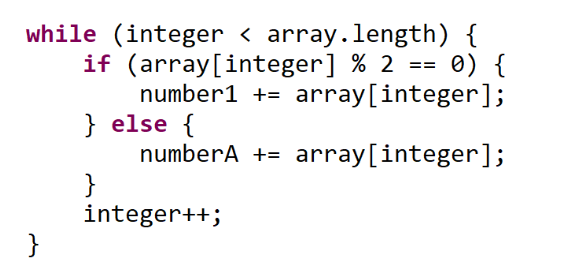
\includegraphics [scale=0.9]
  {figures/4.png}
  \caption{Code snippet with 4-spaces indentation \cite[p. 14]{bauer2017indentations}}
  \label{fig:AnhangsChor}
\end{figure}

\begin{figure} [H]
  \centering
  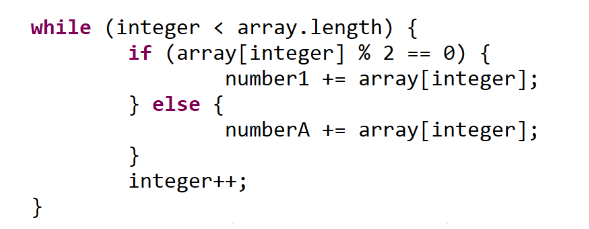
\includegraphics [scale=1]
  {figures/8.png}
  \caption{Code snippet with 8-spaces indentation \cite[p. 14]{bauer2017indentations}}
  \label{fig:AnhangsChor}
\end{figure}


\begin{figure} [H]
  \centering
  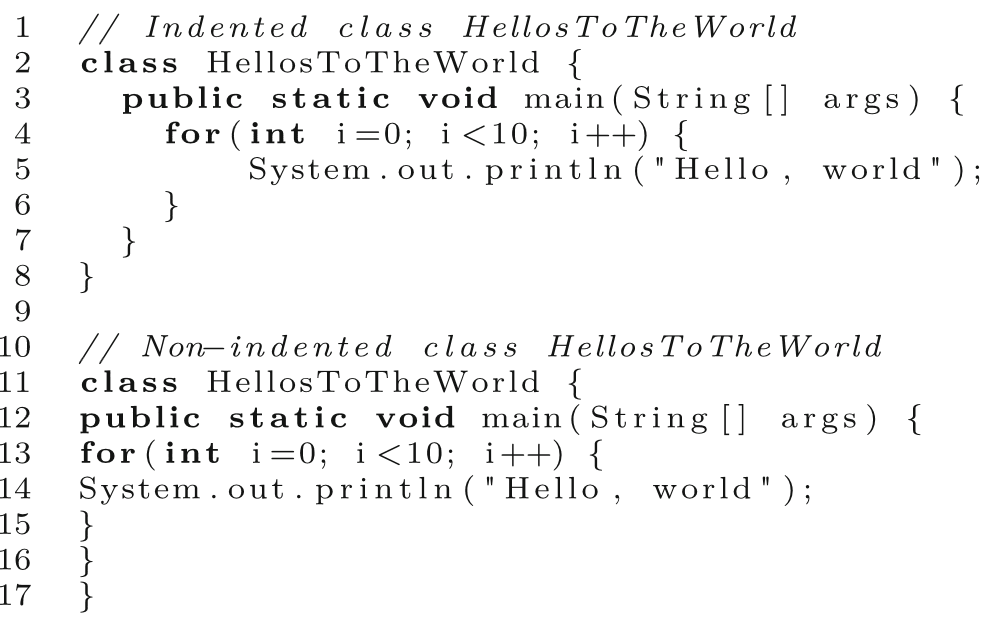
\includegraphics [scale=0.8]
  {figures/indentation_ex.png}
  \caption{Non–indented and indented Java code snippet \cite[p. 4]{hanenberg2024indentation}} 
  \label{fig:AnhangsChor}
\end{figure}

Figure 2.4 presents a Java code snippet, which gives an output the words “Hello, world”  \cite{hanenberg2024indentation}.
In the first code snippet, which is indented, some space is added before the main method and the loop.  In the second code snippet, which is not indented, no spaces are added. The additional space visualizes that particular code lines belong to another fragment. In the non-indented code snippet, it is difficult to detect the code structure. 
 





\section{Commenting}
A comment is an element of source code that provides information \cite{de2011comment}. A comment can consist of names, words, and white spaces.  The goal of a comment is to make the code source code more understandable.  Comments can be defined in different types, regarding their length, their content and their purpose \cite{de2011comment} \cite{de2017investigating}. Comments in source code use natural language, where only a limited part of it is called a sublanguage \cite{de2017investigating}. This sublanguage has specific characteristics. It uses the present tense in imperative or indicative mood. Furthermore, it includes a small set of verbs (is, uses, implements, writes), and personal pronouns are almost never used.

Regarding their length, comments can be defined as line (also called inline) comments and block comments \cite{de2017investigating}. Inline comments consist of one single line. Figure 2.5 presents this type. 

\begin{figure} [H]
  \centering
  
\includegraphics [scale=1]
  {figures/inline.png}
  \caption{Inline comment 
  \cite{de2011comment}}
  \label{fig:AnhangsChor}
\end{figure}

In Figure 2.6 is presented a block comment.  Block comments contain one or more lines. In each programming language, both types can be used. Javadoc is a variation of the block comment provided by Java (Figure 2.7).  Javadoc uses a set of tags that declare information about a method, such as its author and version \cite{de2011comment}.

\begin{figure} [H]
  \centering
  
\includegraphics [scale=1]
  {figures/multiline.png}
  \caption{Block comment
  \cite{de2011comment}}
  \label{fig:AnhangsChor}
\end{figure}

\begin{figure} [H]
  \centering
  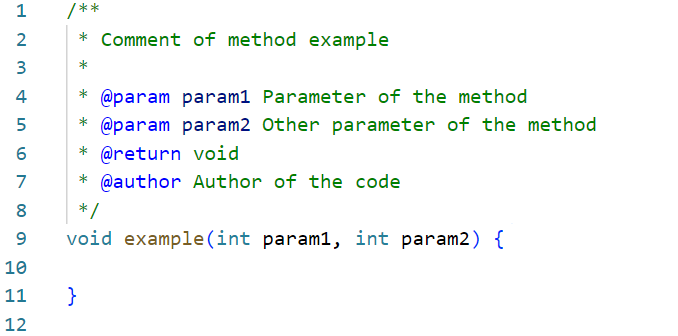
\includegraphics [scale=0.9]
  {figures/javad.png}
  \caption{JavaDoc comment
  \cite{de2011comment}}
  \label{fig:AnhangsChor}
\end{figure}

Regarding the content, comments can be divided into several categories \cite{de2011comment}. The Type category consists of two subcategories: Unit and IntRange. Unit comments present the units of a variable, while IntRange comments the range of values \cite{de2011comment}.
The Interface category includes ErrorReturn comments. This subcategory presents the return values for errors. 
The Code Relationship category includes the subcategories DataFlow and ControlFlow comments: DataFlow comments present dependencies between functions and ControlFlow comments can include information about unreachable code \cite{de2011comment}.
The PastFuture category consists of the subcategories TODO and FIXME comments: these comments indicate that some improvement of the code is needed \cite{de2011comment}.
The Meta category gives information about the authorship. The rest of the comments are considered as part of the Explanation category.


Regarding their purpose and placement in code, comments can be categorized into seven types.  Figure 2.8 presents these types: copyright comments, header comments, member comments, inline comments, section comments, task comments, and code comments. 

\begin{figure}[H]
\centering
\begin{tikzpicture}[
  base/.style={draw, rounded corners, width=4cm, height=1cm, align=center},
  line/.style={draw, -latex},
  node distance=0.6cm
] 

\node[base] (copyright) {Copyright Comments};
\node[base, below=of copyright] (header) {Header Comments};
\node[base, below=of header] (member) {Member Comments};
\node[base, below=of member] (inline) {Inline Comments};
\node[base, below=of inline] (section) {Section Comments};
\node[base, below=of section] (code) {Code Comments};
\node[base, below=of code] (task) {Task Comments};

% Central node (manually placed to center vertically)
\node[base, left=4cm of inline] (main) {Comment Classification};

% Connecting lines
\foreach \node in {copyright, header, member, inline, section, code, task} {
  \draw[line] (main.east) -- (\node.west);
}

\end{tikzpicture}
\caption{Classification of code comments regarding their purpose
\cite{hassan2022code}}
\label{fig:comment_classification}
\end{figure}





Copyright comments are often displayed at the beginning of a file and present information about its license or copyright \cite{steidl2013quality}. Header comments include information about the functionality of the class: class's creator. In Java, these comments are displayed before the declaration of the class \cite{hassan2022code}. Member comments give an overview to the functionality of a method \cite{steidl2013quality}. Inline comments include information about the implementation within a method \cite{steidl2013quality}. Section comments give an overview to group of methods that relate to the same functional aspect \cite{hassan2022code}. Code comments present commented out code, which is not compiled. This type of comments is used for debugging purposes \cite{steidl2013quality}. Task comments are comments, which contain note for a bug or remark \cite{steidl2013quality}.



To analyse the quality of code comments, many aspects of comments should be considered. Four criteria can be determined: coherence, completeness, consistency, and usefulness \cite{steidl2013quality}.
The coherence attribute defines how comments relate to the source code: for instance, member comment should be related to the corresponding method name.
The completeness attribute defines how all relevant information is documented. 
The consistency attribute defines how comments follow a consistent format and language. For instance, when comments are written in the same language, it enhances code readability and comprehension \cite{steidl2013quality}.
The usefulness attribute defines how comments clarify the purpose of the source code. Comments that do not enhance understanding should not be used. 


The length of  comments can influence their completeness \cite{steidl2013quality}. Short comments present less information than longer comments. Figure 2.9 presents a longer code comment, giving more information about the code snippet, while Figure 2.10 visualizes a very short comment.

\begin{figure} [H]
  \centering
  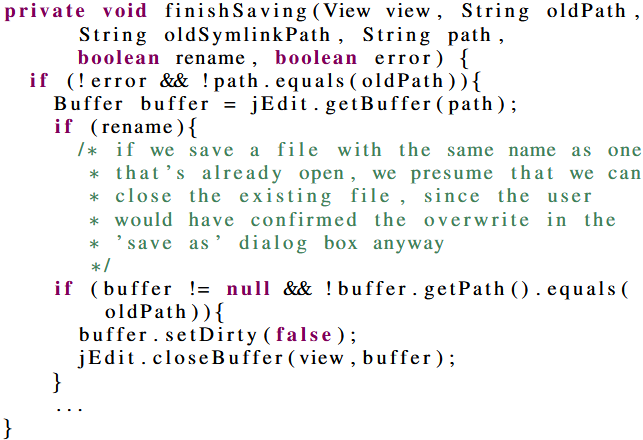
\includegraphics [scale=1]
  {figures/long.png}
  \caption{Example of a long comment
  \cite[p. 6]{steidl2013quality}}
  \label{fig:AnhangsChor}
\end{figure}

\begin{figure} [H]
  \centering
  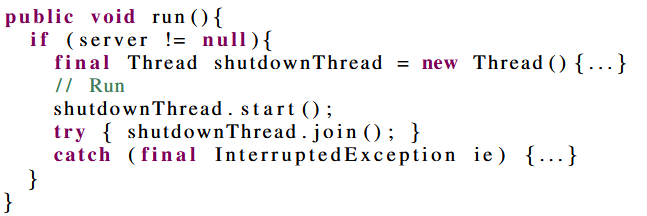
\includegraphics [scale=0.9]
  {figures/run1.png}
  \caption{Example of a short comment
  \cite[p. 6]{steidl2013quality}}
  \label{fig:AnhangsChor}
\end{figure}





\section{Cognitive Load Theory (CLT)}
Cognitive load theory (CLT) is a framework that considers how learning is influenced by the limits of human cognition and investigates the interaction between working memory and long-term memory \cite{duran2022cognitive}. Working memory (WM) is limited, holding information for a short time, while long-term memory is unlimited and holds domain-specific knowledge in schemas  \cite{zavgorodniaia2020measuring}.
Cognitive load refers to the working memory for processing information. 

There are three types of cognitive load: intrinsic load, extraneous load, and germane load. Intrinsic load results from the complexity of the learning task itself, while extraneous load results from how the information is presented \cite{schnotz2007reconsideration}. Germane cognitive load refers to mental effort used for learning, specifically for building schemas \cite{chen2009cognitive}. According to CLT, the three types of loads are additive. Furthermore, CLT guides the design of methods to reduce extraneous load and increase germane load  \cite{chen2009cognitive}. Table 2.3 presents the types of cognitive load.



\begin{table}[ht]
\centering
\small 
\caption{Types of cognitive load \cite{schnotz2007reconsideration} \cite{chen2009cognitive}}
\begin{tabular}{p{0.25\textwidth} | p{0.65\textwidth}}
\hline
\rule{0pt}{1.2em}\textbf{Category} & \textbf{Description} \\[0.5em]
\hline
\rule{0pt}{1.2em}\textbf{Intrinsic Load} & The mental effort required to understand the complexity of the task itself. \\[0.5em]
\hline
\rule{0pt}{1.2em}\textbf{Extraneous Load} & The cognitive effort caused by poor instructional design. \\[0.5em]
\hline
\rule{0pt}{1.2em}\textbf{Germane Load} & The mental effort dedicated to understanding data into long-term memory. \\[0.5em]
\hline
\end{tabular}
\label{tab:cognitive_load}
\end{table}



To measure cognitive load, both subjective and objective measures are used in research.
In subjective measures, the  learner reports on the perceived mental effort, while objective measures use physiological data sources, such as heart rate or eye-tracking technology \cite{duran2022cognitive}. Moreover, objective methods present real-time data.


\section{Theory of Program comprehension}

The process of program comprehension consists of three elements: knowledge-based, external representations, and the assimilation process \cite{kadar2021program}. It explains how a programmer understands a program and is illustrated in Figure 2.11.


\begin{figure} [H]
  \centering
  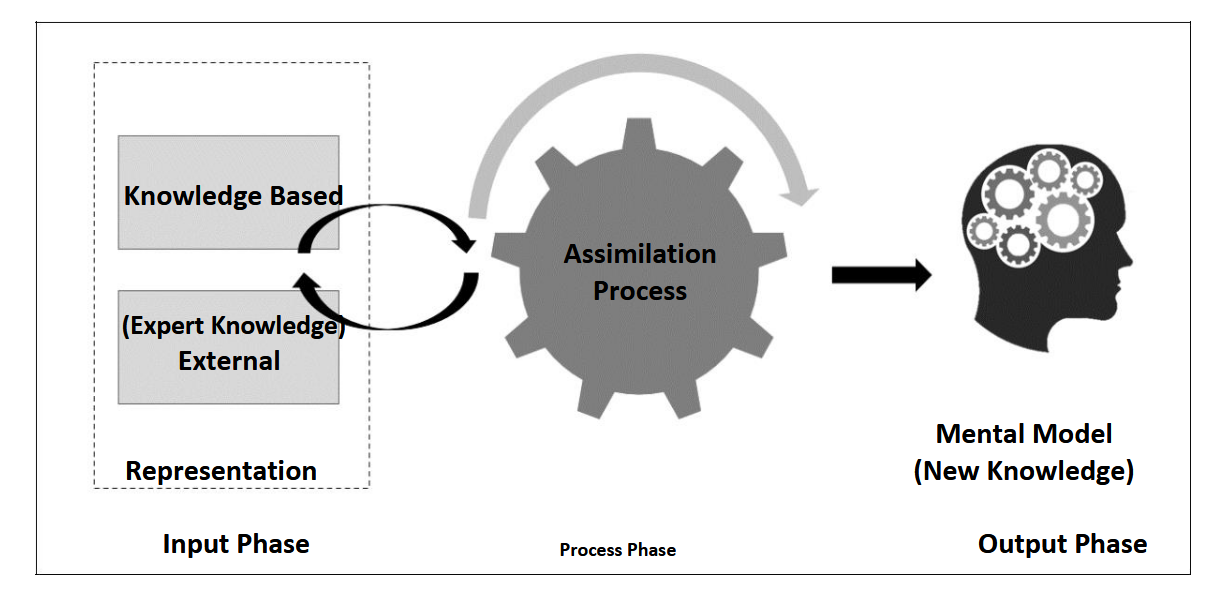
\includegraphics[width=\textwidth]{figures/program_Comprehension_Process.png}
  \caption{The Program comprehension process \cite[p. 5]{kadar2021program}}
  \label{fig:AnhangsChor}
\end{figure}




Knowledge-based refers to the existing knowledge of a programmer. This includes several components: plans and rules of discourse, domain knowledge, beacons, and schemas. Plans and rules of discourse are recognizable patterns in code \cite{fekete2020comprehensive}. Domain knowledge represents the programmer’s knowledge of the task \cite{kadar2021program}.
Beacons are features in the code that give an information about the purpose of the code \cite{fekete2020comprehensive}. Schemas are structures that organize knowledge into units \cite{kadar2021program}. External representations are materials such as system documentation, source code, and tools that provide additional support for program comprehension \cite{kadar2021program}. The assimilation process involves understanding by matching program elements (for example, documentation) with existing knowledge \cite{von1995program}. 



There are three approaches of program comprehension:  top-down, bottom-up, and the integrated metamodel. The top-down approach is goal-oriented. In this approach, the programmer begins with a general hypothesis about what the source code does, based on domain knowledge \cite{storey2005theories}. This hypothesis is later broken down into follow-up hypotheses  \cite{fekete2020comprehensive}. The bottom-up approach defines that programmers read individual code statements and group them into higher-level chunks \cite{storey2005theories}. These chunks are combined until the developer fully understands the program.  Programmers who are not familiar with the code often apply the bottom-up approach \cite{kadar2021program}. The integrated metamodel approach combines both top-down and bottom-up approaches \cite{kadar2021program}.  Programmers choose when to use top-down and bottom-up approach.  The three approaches are shown in Figure 2.12.  



\begin{figure}[H]
\centering
\begin{tikzpicture}[
  every node/.style={font=\small, align=center},
  box/.style={draw, rounded corners, minimum width=4cm, minimum height=1.2cm, fill=blue!10},
  arrow/.style={->, thick}
]

% Top-down approach
\node at (-4,4.5) {\textbf{Top-down approach}};
\node[box] (td1) at (-4,3) {Domain knowledge};
\node[box, below=0.9cm of td1] (td2) {Initial hypothesis};
\node[box, below=0.9cm of td2] (td3) {Follow-up hypotheses};
\node[box, below=0.9cm of td3] (td4) {Code mapping};

\draw[arrow] (td1) -- (td2);
\draw[arrow] (td2) -- (td3);
\draw[arrow] (td3) -- (td4);

% Bottom-up approach
\node at (4,4.5) {\textbf{Bottom-up approach}};
\node[box] (bu1) at (4,3) {Code statements};
\node[box, below=0.9cm of bu1] (bu2) {Chunking};
\node[box, below=0.9cm of bu2] (bu3) {Higher-level abstractions};
\node[box, below=0.9cm of bu3] (bu4) {Program understanding};

\draw[arrow] (bu1) -- (bu2);
\draw[arrow] (bu2) -- (bu3);
\draw[arrow] (bu3) -- (bu4);

% Integrated approach - moved well below
\node at (0,-6.5) {\textbf{Integrated approach}};
\node[box] (int1) at (0,-8) {Combination of \\ Top-down and Bottom-up};

\end{tikzpicture}
\caption{Program comprehension approaches}
\label{fig:comprehension-approaches}
\end{figure}


\section{Eye-tracking}
Eye-tracking technology provides data on how individuals process visual information  \cite{andrzejewska2020development}.
An eye-tracking device collects the eye movements of a participant while the participant works on a task. A stimulus is an object that is needed to perform a task. The eye–mind assumption considers that an individual keeps their gaze on a stimulus until they have understood it \cite{sharafi2015systematic}. Areas of Interest (AOI) define the parts of the stimulus on which the eyes pay attention \cite{sharafi2015systematic}. If certain AOIs help a person complete a task, they are considered relevant. For instance, a relevant AOI in a class diagram is a particular class that the person needs 
\cite{sharafi2015systematic}.

The main terms in eye-tracking technology are fixation and saccade. 
Fixation is a state of stable eye movement for a period of time between 200 to 300 ms \cite{sharafi2015systematic}. This data is encoded with a timestamp and x- and y-coordinates. 
In research, the number of fixations and their duration is usually measured. Saccade is a rapid movement of the eyes, jumping form one point to another \cite{andrzejewska2020development}.
This movement lasts from 30ms to 50ms \cite{obaidellah2018survey}. A scan-path is a set of fixations (of areas of interest), which are in chronological order. Figure 2.13  presents a scanpath with A, B, C, and D as areas of interest  \cite{sharafi2015systematic}.

\begin{figure} [H]
  \centering
  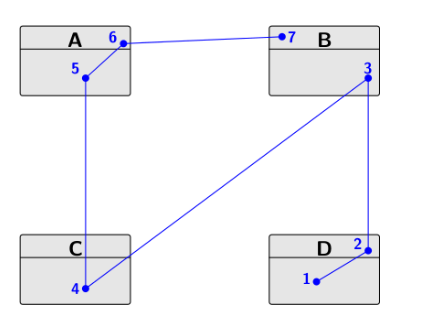
\includegraphics[scale=1.1]{figures/scanp.png}
  \caption{Example of scanpath \cite[p. 4]{sharafi2015systematic}}
  \label{fig:AnhangsChor}
\end{figure}


 
There are several eye-tracking metrics used in research. These metrics help researchers evaluate the level of cognitive processing of people \cite{obaidellah2018survey}. The metrics are defined in four categories: metrics based on fixations,
saccades, pupil size, and scanpath \cite{sharafi2015eye}. Some of the metrics based on fixation are described in Table 2.4.

\begin{table}[H]
\centering
\small % You can change this to \footnotesize or \scriptsize
\caption{Common eye-tracking metrics}
\label{tab:eye_tracking_metrics}
\begin{tabular}{p{0.23\textwidth} | p{0.70\textwidth}}
\hline
\rule{0pt}{1.2em}\textbf{Metric} & \textbf{Description} \\[0.5em]
\hline
\rule{0pt}{1.2em}Fixation Count & The total number of eye fixations on a certain area. A higher fixation count indicates more interest in that area and more effort is spent to complete the task \cite{obaidellah2018survey}. \\[0.5em]
\hline
\rule{0pt}{1.2em}Fixation Duration & One of the most used metrics in eye-tracking technology. It indicates the duration of fixations. A longer fixation duration suggests higher cognitive effort and more attention is required to process the information \cite{junior5005089understanding}. \\[0.5em]
\hline
\rule{0pt}{1.2em}Fixation Rate & The number of fixations per second. A higher fixation rate indicates frequent gaze shifts. A low fixation rate may imply difficulty in processing information or immediate understanding \cite{bauer2017indentations}. \\[0.5em]
\hline
\end{tabular}
\end{table}






To visualize the eye-tracking data, several techniques are used: heatmap, color-coded attention allocation map, and gaze plot. For example, a gaze plot is used to visualize the scanpath. Figure 2.14 presents a gaze plot \cite{sharafi2015systematic}. A heatmap helps to visualize the intensity of fixations. It uses a color spectrum, presenting the gaze patterns of an individual. 
To indicate the intensity of fixation, colors such as red (highest intensity), orange, green, and blue(lowest intensity) are used \cite{sharafi2015systematic}. Figure 2.15 presents a heatmap of a code snippet.  A color-coded attention allocation map maps a color to each word corresponding to the attention level, from light green (lowest attention level) to red (highest level of attention) \cite{sharafi2015systematic}.


\begin{figure} [H]
  \centering
  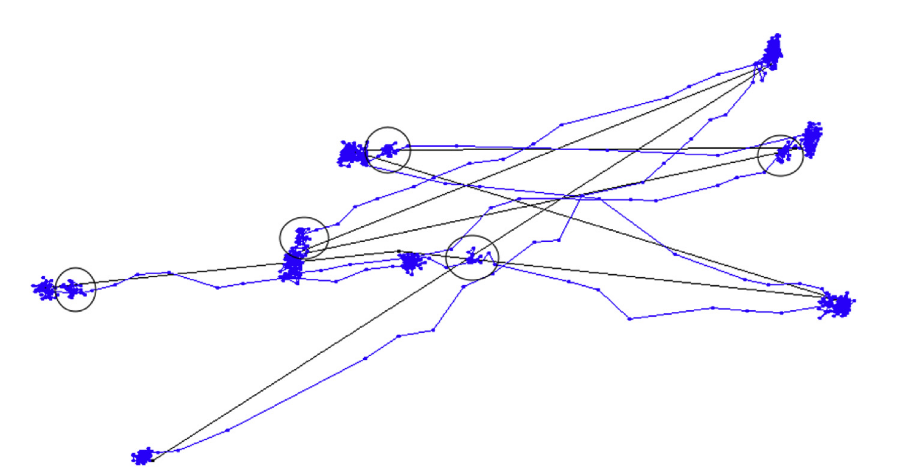
\includegraphics[scale=0.8]{figures/gaze.png}
  \caption{Example of gaze plot \cite[p. 9]{blignaut2019visualization}}
  \label{fig:AnhangsChor}
\end{figure}


\begin{figure} [H]
  \centering
  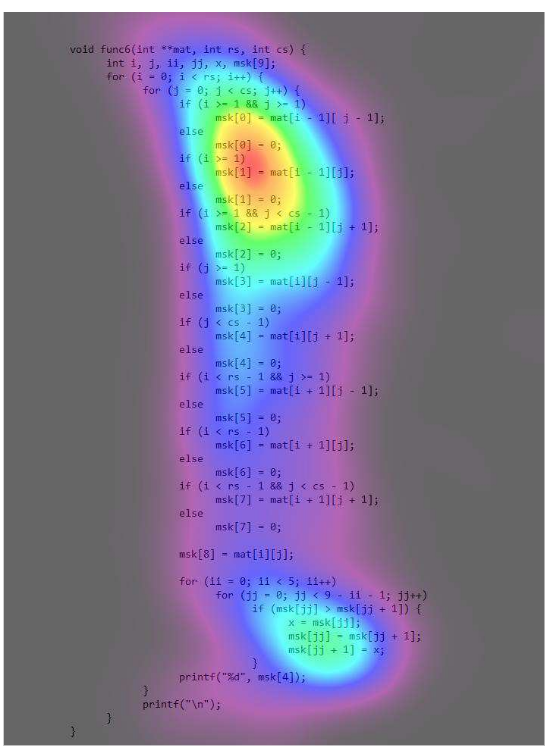
\includegraphics[scale=1]{figures/hm.png}
  \caption{Example of heatmap \cite[p. 13]{jbara2017programmers}}
  \label{fig:AnhangsChor}
\end{figure}



\section{Studies using eye-tracking}


Eye-tracking technology helps to identify the visual patterns of information processing. 
The findings from eye-tracking studies can contribute to improving the learning process \cite{andrzejewska2020development}. Several studies analyze programming comprehension using eye-tracking technology. This chapter reviews key studies, categorizing them based on their focus areas and summarizing their findings.

\subsubsection{Eye-tracking methodologies in software engineering}
The paper by \citet{obaidellah2018survey} investigates the use of eye-tracking technology in computer programming research. A total of 63 relevant studies published between 1990 and June 2017 are analysed \cite{obaidellah2018survey}. The results indicate that eye-tracking technology has been applied to understand programmers' gaze patterns and cognitive processes. The studies reviewed in this paper focus on five main research fields: program comprehension and code understanding, non-code comprehension studies, debugging, requirements traceability, and collaborative programming \cite{obaidellah2018survey}.  The most frequently studied programming language is Java.  
For eye-tracking systems, Tobii is the most commonly used.  Fixation duration and saccades are identified as primary metrics for analysing gaze patterns, and heatmaps are created for visual representation of the results.


\subsubsection{Variable naming conventions and code readability}

The study by \citet{sharif2010eye} investigates whether different variable naming conventions (camel-case and underscore) impact code comprehension and readability.
The task of the participants was to recognize different variable names, while their eye movements were tracked and analysed by researches. 
The findings indicate no significant difference in accuracy between the camel-case and underscore naming conventions \cite{sharif2010eye}. However, underscore identifiers were recognized 20\% faster compared to camel-case identifiers \cite{sharif2010eye}. Moreover, the data from the eye-tracking technology showed that camel-case identifiers led to longer gaze durations, more fixations, and a   higher cognitive load. Furthermore, novice programmers benefited more from the underscore variable naming conventions.   
Overall, the results indicate that underscore variable naming conventions are easier to process visually and potentially improve code readability.   


The eye-tracking study by \citet{broberg2019using} investigates how different variable naming conventions impact code readability.  
The test subjects analyzed code snippets containing variables in Single Word, Single Letter, Camel Case, and Snake Case \cite{broberg2019using}. While explaining the code snippets, their eye movements were tracked. Researchers measured the time participants spent analysing the code and then created heatmaps to visualize their gaze patterns. Furthermore, participants provided feedback on which naming conventions they prefer. The results showed no significant differences in readability using different variable naming conventions \cite{broberg2019using}. However, multi-word conventions like Snake Case and Camel Case were easier to read than Single Letter variable naming conventions \cite{broberg2019using}. The heatmaps presented that test subjects spent more time processing single-letter variables, leading to higher cognitive effort. Moreover, most participants personally found Snake Case and Camel Case easier to understand \cite{broberg2019using}. 
This study presents the role of meaningful variable naming conventions in code and how they improve code readability.   

\subsubsection{Code transformations and their impact on comprehension}
The eye-tracking study by \citet{silva2023evaluating} investigates how different code transformations affect novice programmers’ code comprehension. It focuses on Atoms of Confusion, Refactorings, and ifdef Annotations. 

The findings show that confusing code snippets lead to difficulties in code comprehension and in increased fixations. Figure 2.16 presents the eye-gaze patterns for an obfuscated code snippet using the Conditional Expression atom, while Figure 2.17 illustrates the clarified version of the same snippet \cite{silva2023evaluating}. 
 

\begin{figure} [H]
  \centering
  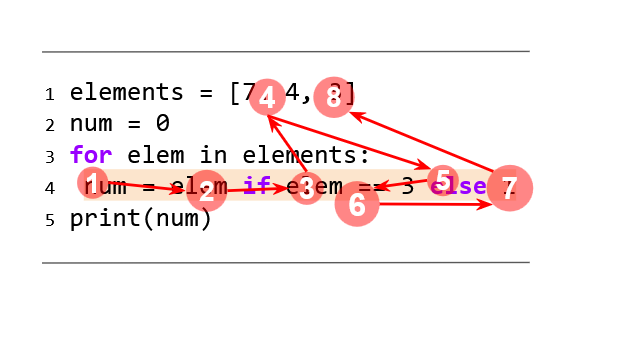
\includegraphics[scale=0.8]{figures/a.png}
  \caption{Obfuscated code snippet \cite[p. 5]{silva2023evaluating}}
  \label{fig:AnhangsChor}
\end{figure}

\begin{figure} [H]
  \centering
  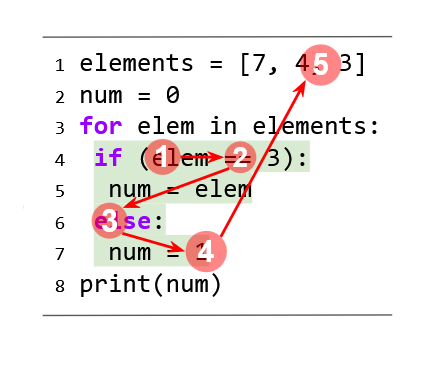
\includegraphics[scale=0.8]{figures/b.png}
  \caption{Clarified version \cite[p. 5]{silva2023evaluating}}
  \label{fig:AnhangsChor}
\end{figure}


\subsubsection{Program comprehension: iteration vs. recursion} 
The study by \citet{aroobaunderstanding} investigates how students perceive recursive and iterative programs and analyzes their cognitive processes and visual attention \cite{aroobaunderstanding}. Moreover, the study inspected whether students followed a top-down approach or a bottom-up approach.
The results present that there was no significant difference between recursive and iterative programs in terms of code comprehension \cite{aroobaunderstanding}.  However, visual attention differed between iteration and recursion. 

\subsubsection{Cognitive load and code complexity} 

The eye-tracking paper by \citet{abbad2022estimating} investigates how to identify difficult areas of code for programmers.  Participants were given different Java code snippets and mentioned the areas of the code they found difficult \cite{abbad2022estimating}. Researchers compared the eye-tracking data with the parts marked as complicated by the participants. With the collected data, they trained machine learning models to forecast which parts of the code would challenge code comprehension \cite{abbad2022estimating}. The researchers achieved more than 86\% accuracy in predicting complicated parts of code snippets. The study highlights its future usage for developing tools that can enhance code review and adaptive e-learning.  



\subsubsection{Code structure and indentation} 


The eye-tracking study by \citet{bauer2017indentations} investigates how indentation affects comprehension. Participants analyzed Java code snippets with different levels of indentation: 0, 2, 4, and 8-space. The study is relevant to this thesis, as one of the research questions is how code with different  indentation levels impacts comprehension. The results of the study by \citet{bauer2017indentations} did not present a significant relationship between comprehension and indentation. However, the most correct answers were given when the participants analyzed the code with 4-space indentation. Furthermore, the results indicated that the 8-space indentation was rated the easiest to read level of indentation, but did not improve the accuracy of correct answers \cite{bauer2017indentations}. In general, the eye-tracking data did not show significant differences in gaze patterns between different indentation levels, and the study highlights the need for further investigation. 


Another study by \citet{yorimoto2024quantitative} investigates how indentation affects the comprehension of code. The students were given code tasks with different levels of indentation: 0 character, 4 character, and random indentation \cite{yorimoto2024quantitative}. The researchers measured the eye movements and cognitive load of the participants. The results showed increased confusion and cognitive load when students analyzed code with unstructured indentation \cite{yorimoto2024quantitative}. Furthermore, 4-character indentation resulted in more precise but longer focus on code areas. The study mentions that indentation had little impact on small code tasks and highlights that further investigation is needed \cite{yorimoto2024quantitative}.  

\subsubsection{Code comments} 

The study by  \citet{bakhuizen2019comments} investigates how incorrect code comments affect programmers' code comprehension. The study is relevant to this thesis, as one of the research questions is how code with different  commenting formats impacts comprehension and cognitive load.  Participants in the study by  \citet{bakhuizen2019comments} analyzed code containing missing, incorrect, or correct comments.
The researchers used eye-tracking technology to measure how often participants read code comments. The results indicate that participants read code comments as frequently as the code \cite{bakhuizen2019comments}. Furthermore, incorrect comments can negatively affect code comprehension, leading to misinterpretations of the code. Moreover, accurate and correct comments are useful when they provide correct information for unknown functions. 

The reviewed key studies present that different code formats and structures can affect code comprehension. Moreover, they highlight the use of eye-tracking technologies to investigate comprehension processes.  Eye-tracking data provide insights into how expert and novice programmers perceive different code structures and styles. There has been made significant progress in investigating the comprehension and readability of code by programmers.  However, there is a lack of deeper research on how indentation and comments influence the comprehension.  Previous research investigates indentation and comments separately, but in this thesis, they are inspected together. Moreover, the use of both eye-tracking data and subjective data offers more comprehensive insights. Many studies focus on experienced programmers, while this thesis focuses on CS1 students. 





\chapter{Study Design}

This chapter presents the study design, its approach, and the technical setup.  It also describes the selection of code snippets and variables that are used for evaluation.

\section{Methodology}

\subsection{Study approach} The data in this study are gathered using two methods: eye-tracking technology and a questionnaire. This approach provides both objective and subjective data, as well as quantitative and qualitative data. Figure 3.1 presents an overview of how the data are gathered. 



\begin{figure} [H]
  \centering
  
  \caption{Study data}
  \label{fig:AnhangsChor}



\begin{tikzpicture}[node distance=1cm and 3cm, align=center, font=\footnotesize]


\tikzstyle{box} = [draw, minimum height=3cm, minimum width=4cm, text width=3.5cm, inner sep=5pt]

\node (eyeTracking) [box] {Eye-tracking  data \\[5mm] $\rightarrow$ Measures gaze};
\node (questionnaire) [box, right=of eyeTracking] {Questionnaire data \\[5mm] $\rightarrow$ Subjective data  };

\node (study) [box, below=2cm of $(eyeTracking)!0.5!(questionnaire)$, text width=7cm, align=center] {The study \\[5mm] $\rightarrow$ Both data give a complete view}; 

\draw[->] (eyeTracking) -- (study);
\draw[->] (questionnaire) -- (study);

\end{tikzpicture}

\end{figure}

 

Eye-tracking technology gives objective data. Using this type of data, it can be tracked which parts of the code are seen and for how long. Questionnaire can give qualitative and quantitative data (using Likert scale questions). Moreover, a questionnaire can give subjective data about the participants (using open-ended questions). The participants report their perceived code comprehension.  
Previous research has also used both methods to gather data for a deeper code comprehension (see Chapter 2: Literature review). 


The study is conducted in German. It is used a within-subjects design, ensuring that each participant is exposed to all conditions.
The study consists of two formats: an eye-tracking study (offline study) and an online study without eye-tracking. Figure 3.2 presents the structure of the study. 
\begin{figure}[H]
  \centering
  \caption{Study structure}
  \label{fig:AnhangsChor}

\begin{tikzpicture}[node distance=3.5cm, font=\footnotesize, align=center]

% Top layer
\node (eyeTracking) [draw, minimum height=2.5cm, minimum width=3cm, text width=2.6cm] {Eye-tracking};
\node (questionnaire) [draw, minimum height=2.5cm, minimum width=3cm, text width=2.6cm, right=2.2cm of eyeTracking] {Questionnaire1};
\node (questionnaire2) [draw, minimum height=2.5cm, minimum width=3cm, text width=2.6cm, right=2.2cm of questionnaire] {Questionnaire1};

% Second layer
\node (offlineStudy) [draw, minimum height=2.5cm, minimum width=3cm, text width=2.6cm, below=3.5cm of eyeTracking] {Offline study};
\node (onlineStudy) [draw, minimum height=2.5cm, minimum width=3cm, text width=2.6cm, below=3.5cm of questionnaire2] {Online study};

% Third layer
\node (study) [draw, minimum height=2.5cm, minimum width=6.5cm, text width=6.2cm, below=3.5cm of $(onlineStudy)!0.5!(offlineStudy)$] {The study};

% Arrows
\draw[->] (eyeTracking) -- (offlineStudy);
\draw[->] (questionnaire) -- (offlineStudy);
\draw[->] (questionnaire2) -- (onlineStudy);
\draw[->] (onlineStudy) -- (study);
\draw[->] (offlineStudy) -- (study);

\end{tikzpicture}
\end{figure}


Both the offline and online study use the same questionnaire. The eye-tracking study (offline study) gathers data using eye-tracking technology and a questionnaire. The eye-tracking device gives objective qualitative data as output and the questionnaire gives both objective and subjective data, as well as quantitative and qualitative data as output.  By combining both methods, the findings indicate whether the questionnaire data aligns with the eye-tracking data.
The online study without eye-tracking gathers data using only a questionnaire.  Using both formats, the study provides a more comprehensive overview of how computer science students perceive code. 



\subsection{Code snippet selection}

The programming language used for the code snippets is Java, since it is a widely used language.  Additionally, most students who participated in the study are from Ludwig Maximilian University of Munich, where Java is a key part of many computer science courses. The following code snippets formats are used in the study:



\begin{enumerate}
    \item \textbf{Comment formats:}
    \begin{itemize}
        \item \textbf{No comments:} Code snippet without any comments.
        \item \textbf{Minimal comments:} Code snippet with minimal and essential comments.
        \item \textbf{Helpful comments:} Code snippet with meaningful comments.
        \item \textbf{Redundant comments:} Code snippet with unnecessary comments.
    \end{itemize}
    
    \item \textbf{Levels of indentations:}
    \begin{itemize}
        \item \textbf{0-spaces indentation (no indentation):} Code snippet without indentation.
        \item \textbf{4 spaces indentation:} Code snippet with 4-spaces indentation.
        \item \textbf{Random indentation:} Code snippet with random indentation.
    \end{itemize}
\end{enumerate}

Figure 3.3  presents an example for one code snippet with minimal comments. All code snippets used in the study are provided in Appendix A.

\begin{figure} [H]
  \centering
  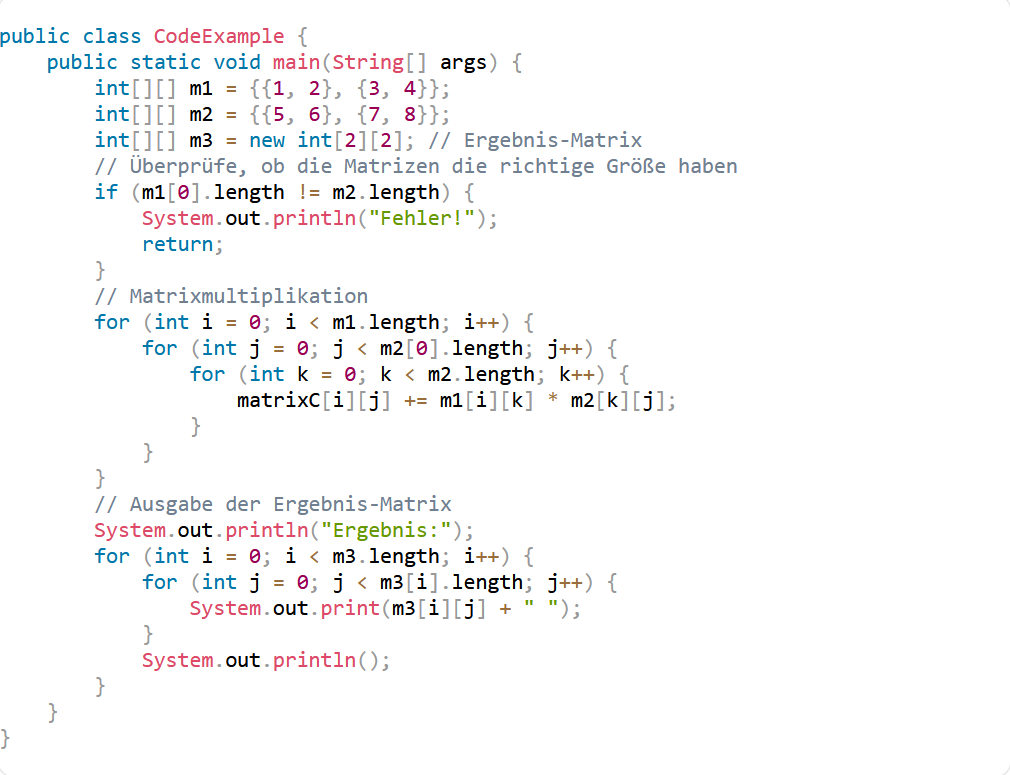
\includegraphics[scale=1]{figures/codeb.png}
  \caption{Code snippet example }
  \label{fig:AnhangsChor}
\end{figure}




\subsection{Justification of code snippets selection }
The code snippets are collected from programming lectures conducted at LMU University and adapted from the computer science exercises \cite{lmu_programming_lectures}. The main reason why the snippets were selected from lectures is that they provide widely used examples. 
The selection of the code snippets formats is based on the findings from previous research. Previous studies have concluded that indentation levels and comment styles influence code readability and comprehension  (see Chapter 2: Literature review). Therefore, the snippets in this study are designed to investigate how different levels of indentation and different commenting formats affect code comprehension.  Moreover, the code snippets are simple enough and no additional knowledge is required. Furthermore, the usage of loops and conditionals in the snippets can require different levels of cognitive processing.  An overview of the code snippets formats is presented in Table 3.1.   

\begin{table}[ht]
\centering
\small
\caption{Overview of code snippet formats}
\begin{tabular}{|p{6cm}|p{6cm}|}
\hline
\multicolumn{2}{|c|}{\rule{0pt}{1.2em}\textbf{Commenting formats}} \\[0.5em]
\hline
\rule{0pt}{1.2em}\textbf{Type} & \textbf{Control variable} \\[0.5em]
\hline 
\rule{0pt}{1.2em}No comments & 4-space indentation \\[0.5em]
\hline
\rule{0pt}{1.2em}Minimal comments & 4-space indentation \\[0.5em]
\hline
\rule{0pt}{1.2em}Helpful comments & 4-space indentation \\[0.5em]
\hline
\rule{0pt}{1.2em}Redundant comments & 4-space indentation \\[0.5em]
\hline
\multicolumn{2}{|c|}{\rule{0pt}{1.2em}\textbf{Indentation levels}} \\[0.5em]
\hline
\rule{0pt}{1.2em}\textbf{Type} & \textbf{Control variable} \\[0.5em]
\hline
\rule{0pt}{1.2em}No indentation & No comments \\[0.5em]
\hline
\rule{0pt}{1.2em}4-space indentation & No comments \\[0.5em]
\hline
\rule{0pt}{1.2em}Random indentation & No comments \\[0.5em]
\hline
\end{tabular}
\label{tab:snippet_control}
\end{table}



Each snippet is focused on one dimension at a time (levels of indentation or commenting formats). This enables a simple analysis and comparison across the different formats. The study has seven different code snippets. It combines three levels of indentation and four types of commenting styles. For the commenting formats, four types are selected.  The role of the snippet with no comments is to investigate whether code can be understood without any additional information.  Minimal comments test whether minimal information is better than none and improves comprehension, or makes it difficult for understanding.
Helpful comments investigate whether meaningful information enhances deeper code comprehension. The helpful comments were designed based on the theoretical findings discussed in the Chapter Literature Review: these comments explain the purpose of the code snippets without adding unnecessary information. Redundant comments aim to explore whether unnecessary comments make the code difficult to understand, potentially causing cognitive overload.


For the indentation, three levels were selected. 
The role of the code snippet with no indentation is to investigate how the absence of indentation influences code readability and whether it causes cognitive overload.
The 4-space indentation is defined as the standard indentation in research and is used to explore whether it enhances deeper code readability.  
Random indentation tests whether using different indentation across the code makes the snippet difficult to read and causes cognitive overload.



For the commenting formats snippets, the snippets have 4-space indentation. This ensures that the focus is only on the comments. This indentation is defined as a "control variable", which allows deeper comparison across the different commenting formats. 
For the indentation code snippets, the snippets consist of no comments. This ensures that the focus is only on the indentation. Here, the no comment format is also defined as a "control variable", which allows a deeper comparison across the different indentation levels. 

\subsection{Research variables}
To evaluate the results from the study, two types of variables are used - independent variables and dependent variables. The independent variables in the study are variables that are manipulated. In the study   two independent variables are used - Commenting format and Indentation level.

\begin{enumerate}
     \item Commenting format: The key role of this independent variable is to investigate how commenting format influences code comprehension. This variable consists of four different types: None (no comments are included in the code), Minimal (these comments include only essential information), Helpful (these comments provide meaningful explanations), Redundant (these comments explain obvious parts of the code). 

    \item Indentation level: The key role of this independent variable is to investigate how indentation influences code comprehension and readability. This variable consists of four different types: No indentation (the code has no indentation), 4-spaces indentation (the code has four spaces indentation), Random indentation (the code has inconsistent indentation). 
\end{enumerate}


The independent variables influence the dependent variables. The dependent variables are measured and the outcomes help to investigate how the independent variables influence code comprehension.


In this thesis are defined the following dependent variables: Comprehension score, Comment quality score, Indentation quality score, Confidence rating and  Response time per code snippet. An overview is presented in Table 3.2.


\begin{longtable}{|p{5.5cm}|p{8.5cm}|}
\caption{Description of variables} \label{tab:variables} \\

\hline
\textbf{Variable} & \textbf{Description} \\
\hline
\endfirsthead

\hline
\textbf{Variable} & \textbf{Description} \\
\hline
\endhead

\hline
\parbox[t]{5.5cm}{\vspace{0.3em}Comprehension score\vspace{0.5em}} &
\parbox[t]{8.5cm}{\vspace{0.3em}This variable was derived from Question 3: "How understandable is the code for you?". Participants rate the code on a Likert scale, where 1 = "Not understandable" and 5 = "Very understandable".\vspace{0.5em}} \\
\hline

\parbox[t]{5.5cm}{\vspace{0.3em}Comment quality score\vspace{0.5em}} &
\parbox[t]{8.5cm}{\vspace{0.3em}This variable was derived from Question 4: "How do you assess the commenting of the code?". Participants rate the code on a Likert scale, where 1 = "Confusing" and 5 = "Very helpful".\vspace{0.5em}} \\
\hline

\parbox[t]{5.5cm}{\vspace{0.3em}Indentation quality score\vspace{0.5em}} &
\parbox[t]{8.5cm}{\vspace{0.3em}This variable was derived from Question 5: "How do you assess the indentation of the code?". Participants rate the indentation of the code on a Likert scale, where 1 = "Unreadable" and 5 = "Very easy to read".\vspace{0.5em}} \\
\hline

\parbox[t]{5.5cm}{\vspace{0.3em}Response time per code snippet\vspace{0.5em}} &
\parbox[t]{8.5cm}{\vspace{0.3em}This variable measures how long (in minutes) each participant took to view a code snippet and answer its corresponding five questions.\vspace{0.5em}} \\
\hline

\parbox[t]{5.5cm}{\vspace{0.3em}Confidence rating\vspace{0.5em}} &
\parbox[t]{8.5cm}{\vspace{0.3em}This variable was derived from Question 2: “How confident are you in your answer to the first question?” (the first question is related to the function of the corresponding code snippet). Participants rate their code confidence on a Likert scale, where 1 = "Not confident" and 5 = "Very confident".\vspace{0.5em}} \\
\hline

\end{longtable}


\subsection{Technical setup}


The eye-tracking study (offline study) was conducted at LMU, Munich. As eye-tracking device was used a Pupil Labs Core. This device contains glasses with three cameras. The glasses were connected to a laptop, running Pupil Capture software v.3.5.1. This software ensures calibration and recording of eye movements. The glasses were individually calibrated for each participant. The laptop was placed on a desk. During the study, participants read the snippets and answered the questionnaire on the same laptop. This setup ensured minimal distractions. The technical setup is presented in Figure 3.4. 

\begin{figure} [H]
  \centering
  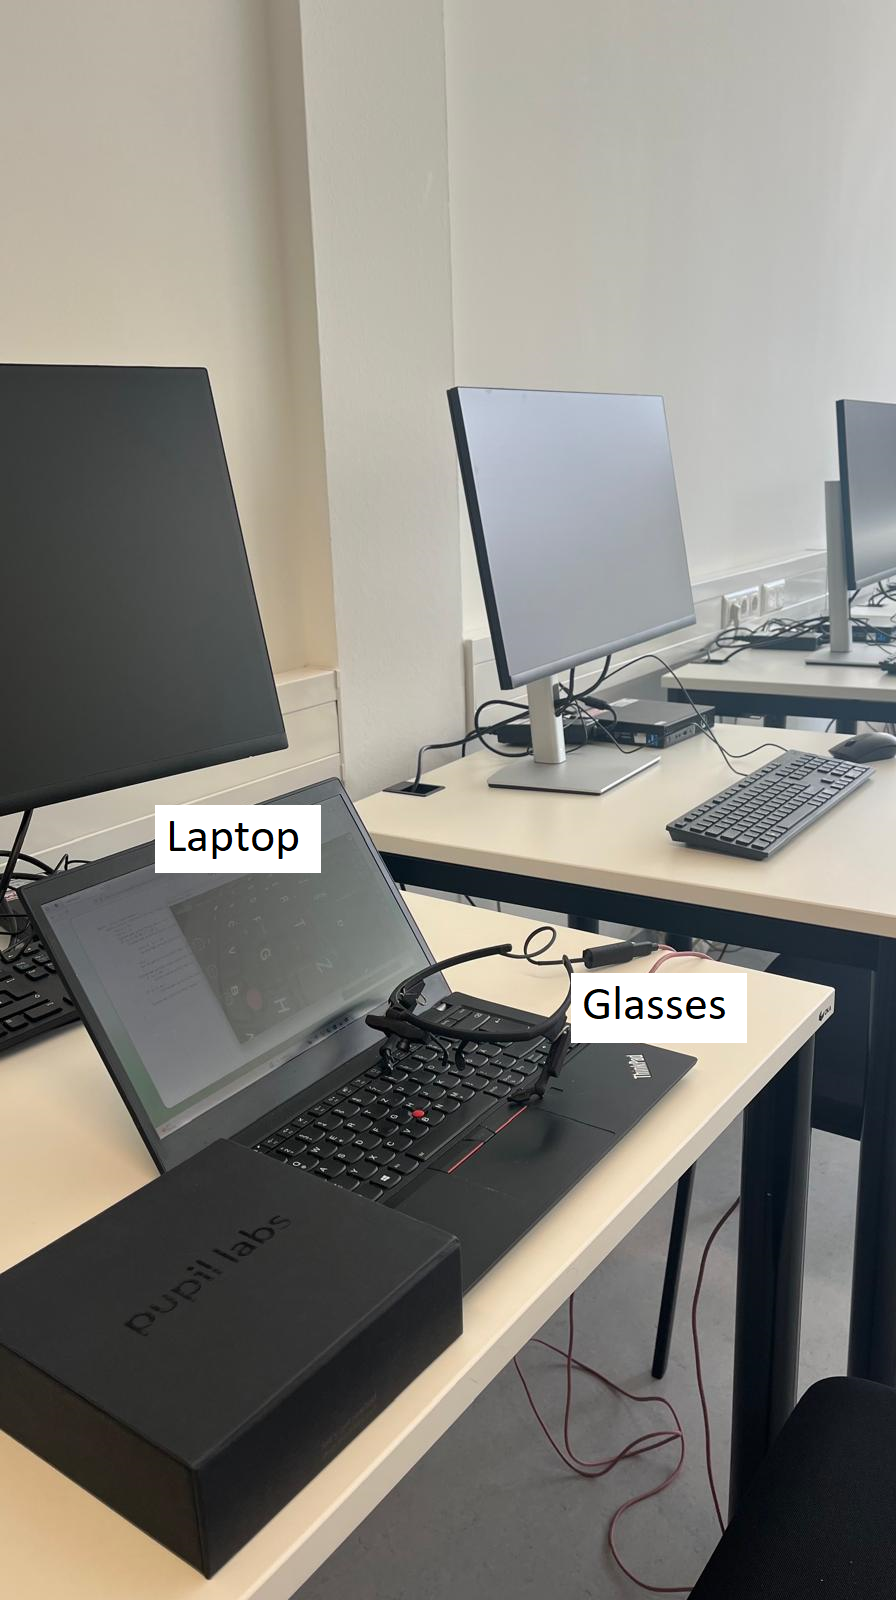
\includegraphics[scale=0.5]{figures/setup.png}
  \caption{Technical setup }
  \label{fig:AnhangsChor}
\end{figure}

\subsection{Recruitment of participants}

Participants were recruited from computer science courses at LMU. The study focused on novice programmers, particularly CS1 students. Participation was voluntary.

\section{Questionnaire design}


\subsection{First part of questionnaire}



The questionnaire was implemented as a website using Python 3.12.3. The design uses a green color, which is the official color of LMU, Munich. 
Figure 3.5 shows the design of the first part of the questionnaire. The first part of the questionnaire gives general information about the participants. 
Participants provide details about their field of study, as well as information about their academic background: their programming experience level and experience in Java. 
\begin{figure} [H]
  \centering
  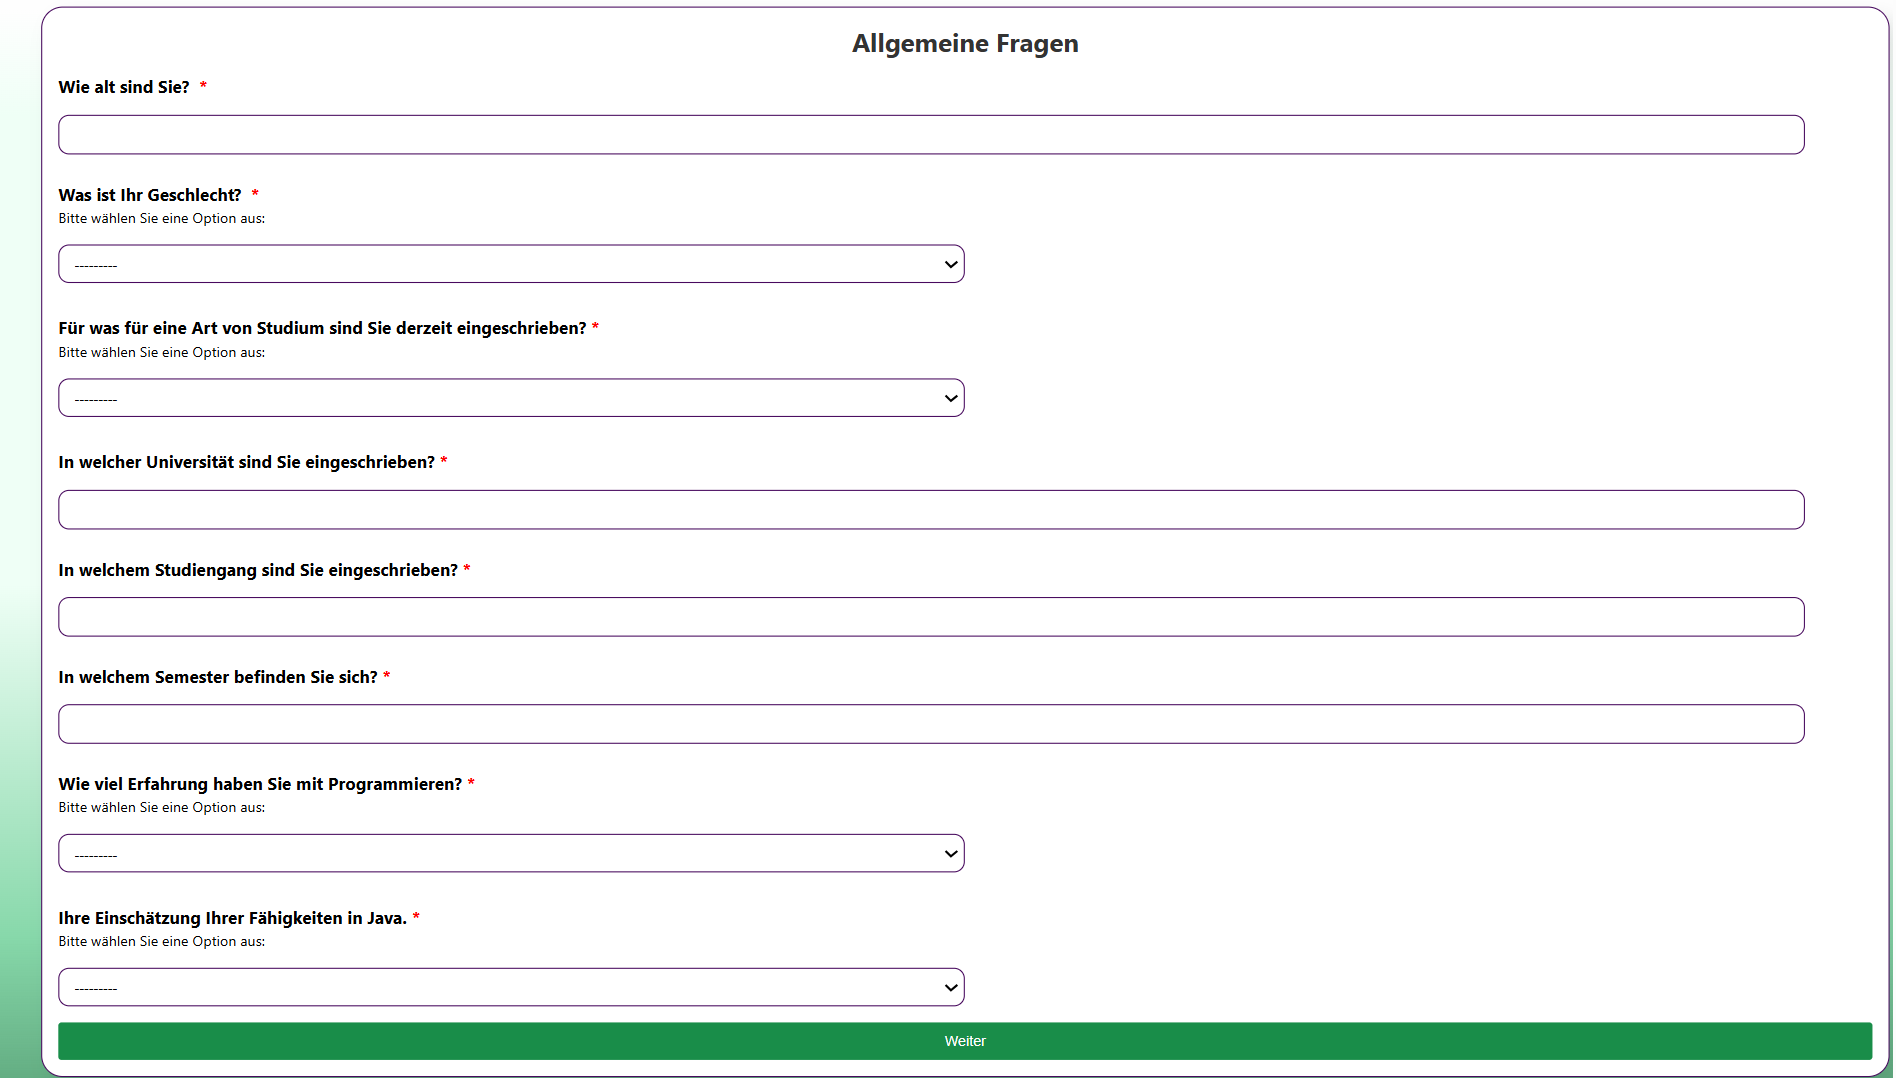
\includegraphics[scale=0.45]{figures/allgemein.png}
  \caption{First part of questionnaire}
  \label{fig:AnhangsChor}
\end{figure}


\subsection{Main part of questionnaire}

In the main part of the questionnaire are shown seven different code snippets. Their order is randomized to avoid bias. Each code snippet presents a different level of indentation and a different type of comment format.
Participants answer five questions corresponding to each code snippet. These questions are related to the code snippet’s function, ratings of the code comprehension, code indentation, and code commenting. Figure 3.6 shows the design of the main part of the questionnaire.


\begin{figure} [H]
  \centering
  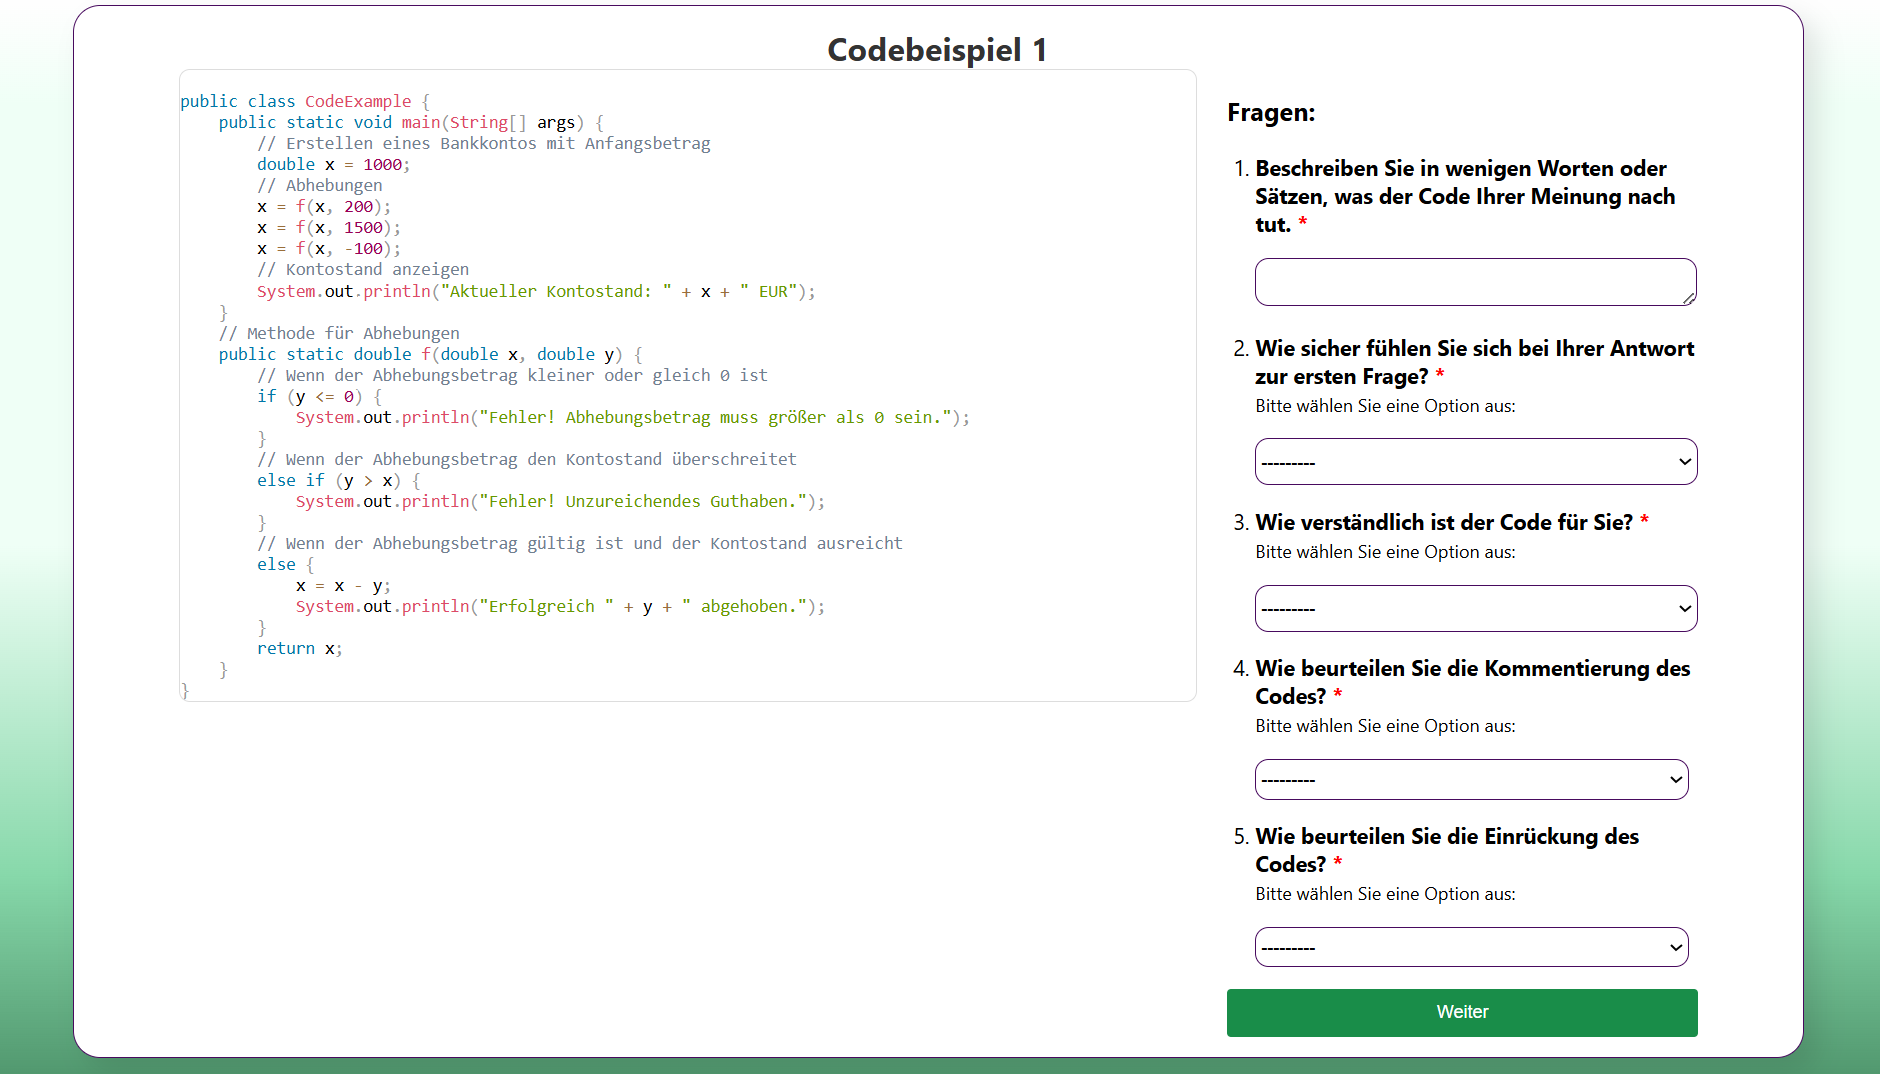
\includegraphics[scale=0.45]{figures/main_p.png}
  \caption{Main part of questionnaire}
  \label{fig:AnhangsChor}
\end{figure}



\subsection{Final part of the questionnaire}
In the last part of the questionnaire, participants give their opinions on code indentation and code comments guidelines. They describe what they take into consideration when defining poorly commented and well-commented code. Moreover, they explain which code indentation style they use.  Figure 3.7 shows the design of the last part of the questionnaire.


\begin{figure}  [H]
  \centering
  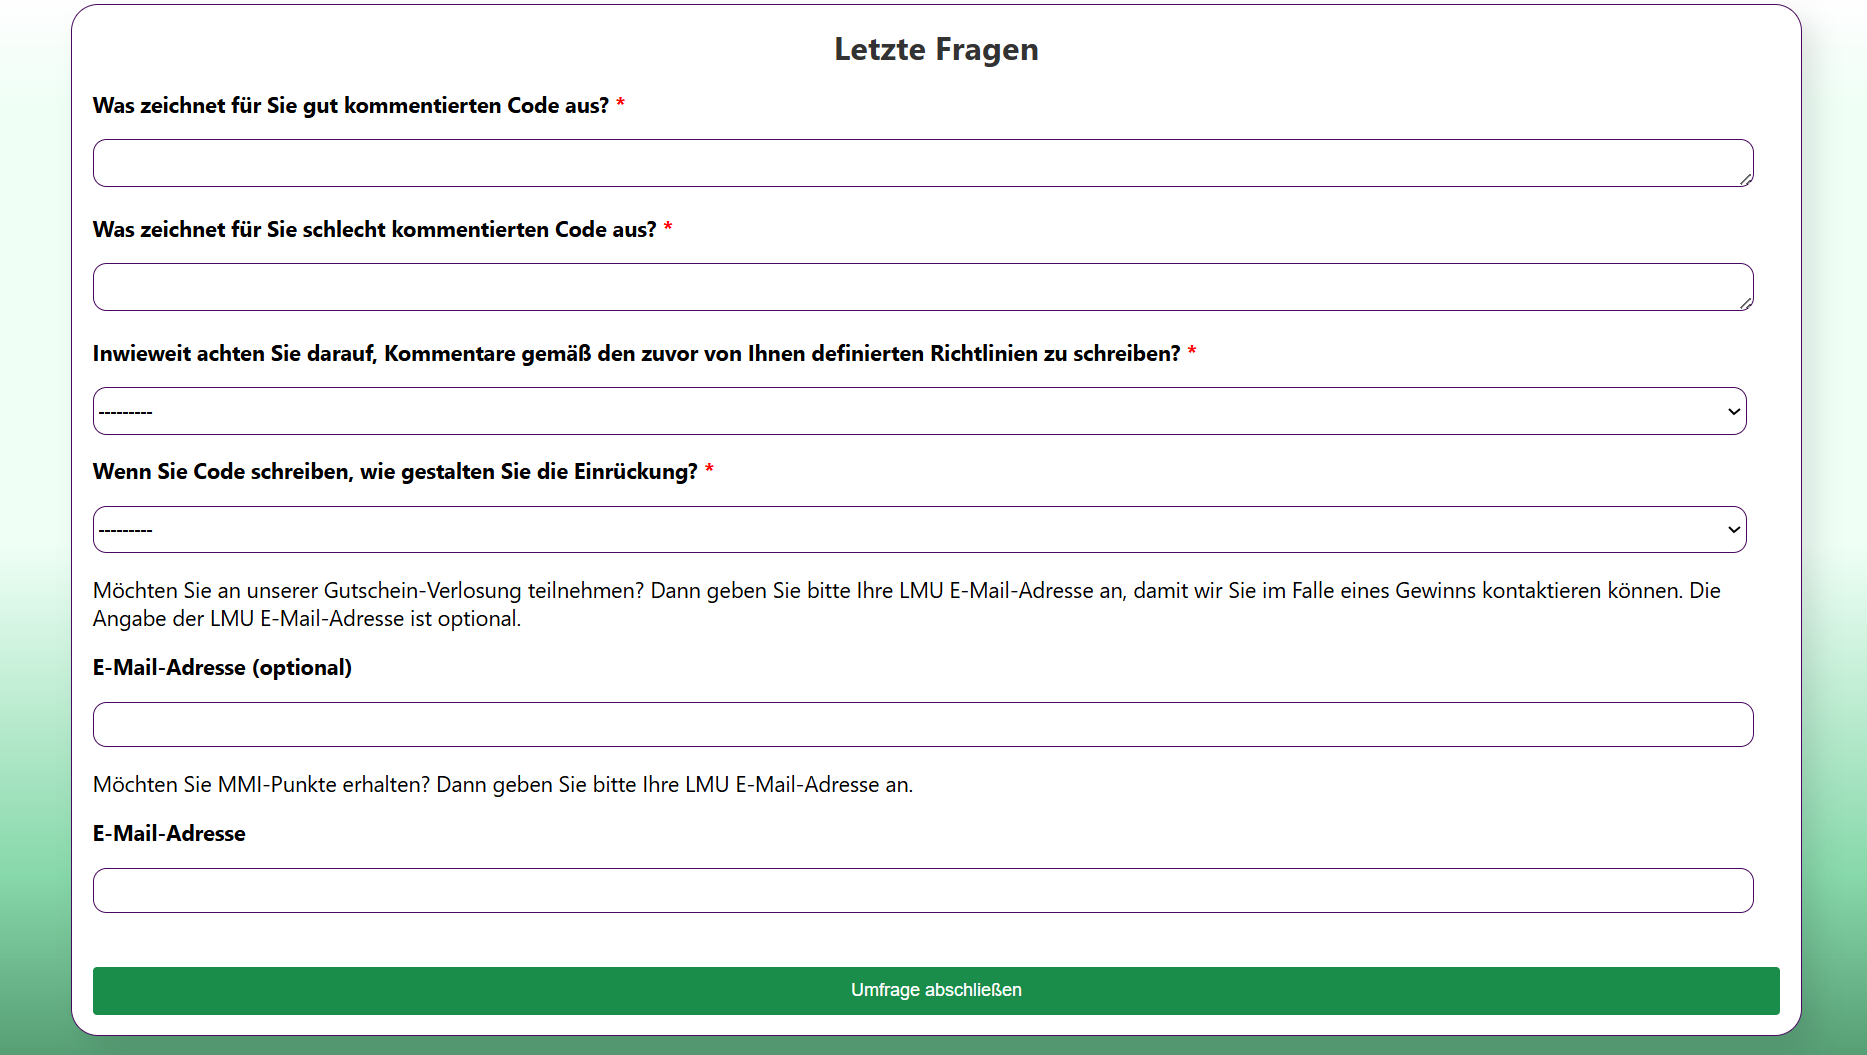
\includegraphics[scale=0.45]{figures/last_part.png}
  \caption{Final part of the questionnaire}
  \label{fig:AnhangsChor}
\end{figure}


 
\section{Procedure}

The eye-tracking study (offline study) and the online study without eye-tracking formats are constructed similarly, but have some differences. The detailed procedure for both formats is outlined below.

\subsection{Procedure for the eye-tracking study}

Before conducting the eye-tracking study, a pilot study with one participant was performed. The purpose of this pilot study was to ensure that the questionnaire was clear and that the eye tracking setting worked properly. Based on the result, small improvements were made.



\begin{enumerate}
    \item \textbf{Introduction:} At the beginning, participants answered several warm-up questions: “How are you feeling today? Do you have any experience with reading source code? Do you have any experience with eye-tracking studies?”. Then, participants were informed about the purpose of the study, data collection methods, and their right to withdraw from the study at any time.

    \item \textbf{Calibration of the eye-tracking system:} 
    Eye-tracker calibration is essential to ensure that the eye-tracking device correctly detects participants’ eyes and eye movements. Before calibration, participants put on the eye-tracking device and adjust three cameras: one for the screen, one for the right eye, and one for the left eye. It is essential to ensure that both eyes are correctly detected. After the adjustment is performed, participants are asked to focus on several specific points on the screen. The system recorded their gaze. In some cases, calibration errors occurred and recalibration was required. After the calibration is completed, the eye-tracking system started recording participants’ gaze. Participants read all relevant information themselves and then proceed to the questionnaire.
    
    \item \textbf{First part of questionnaire:}  
    Participants answered several questions providing demographic, background, and programming experience information. When the students filled out these questions, they proceeded to the main part of the questionnaire - code comprehension task.

    \item \textbf{Main part of questionnaire - code comprehension task:}  Each participant was shown seven different code snippets. The order of the code snippets was randomized in order to avoid bias. The participants read each code snippet, while the eye-tracking device recorded their gaze movements, saccades, fixations, and pupil dilation. After reading each code snippet, students answered five questions. These questions are related to the corresponding code snippet. Moreover, their answers and response times were recorded.

    \item \textbf{Final part of the questionnaire:} 
    The participants answered several questions providing information about their opinions on commenting and indentation in code.

    \item \textbf{End of the study:} 
    Participants were asked to give feedback on the difficulty level of the code snippets. Furthermore, the students mentioned their opinions on code readability and code comprehension. Additionally, they shared the challenges they faced during the eye-tracking study. Figure 3.8 shows a participant conducting the eye-tracking study.


\begin{figure} [H]
  \centering
  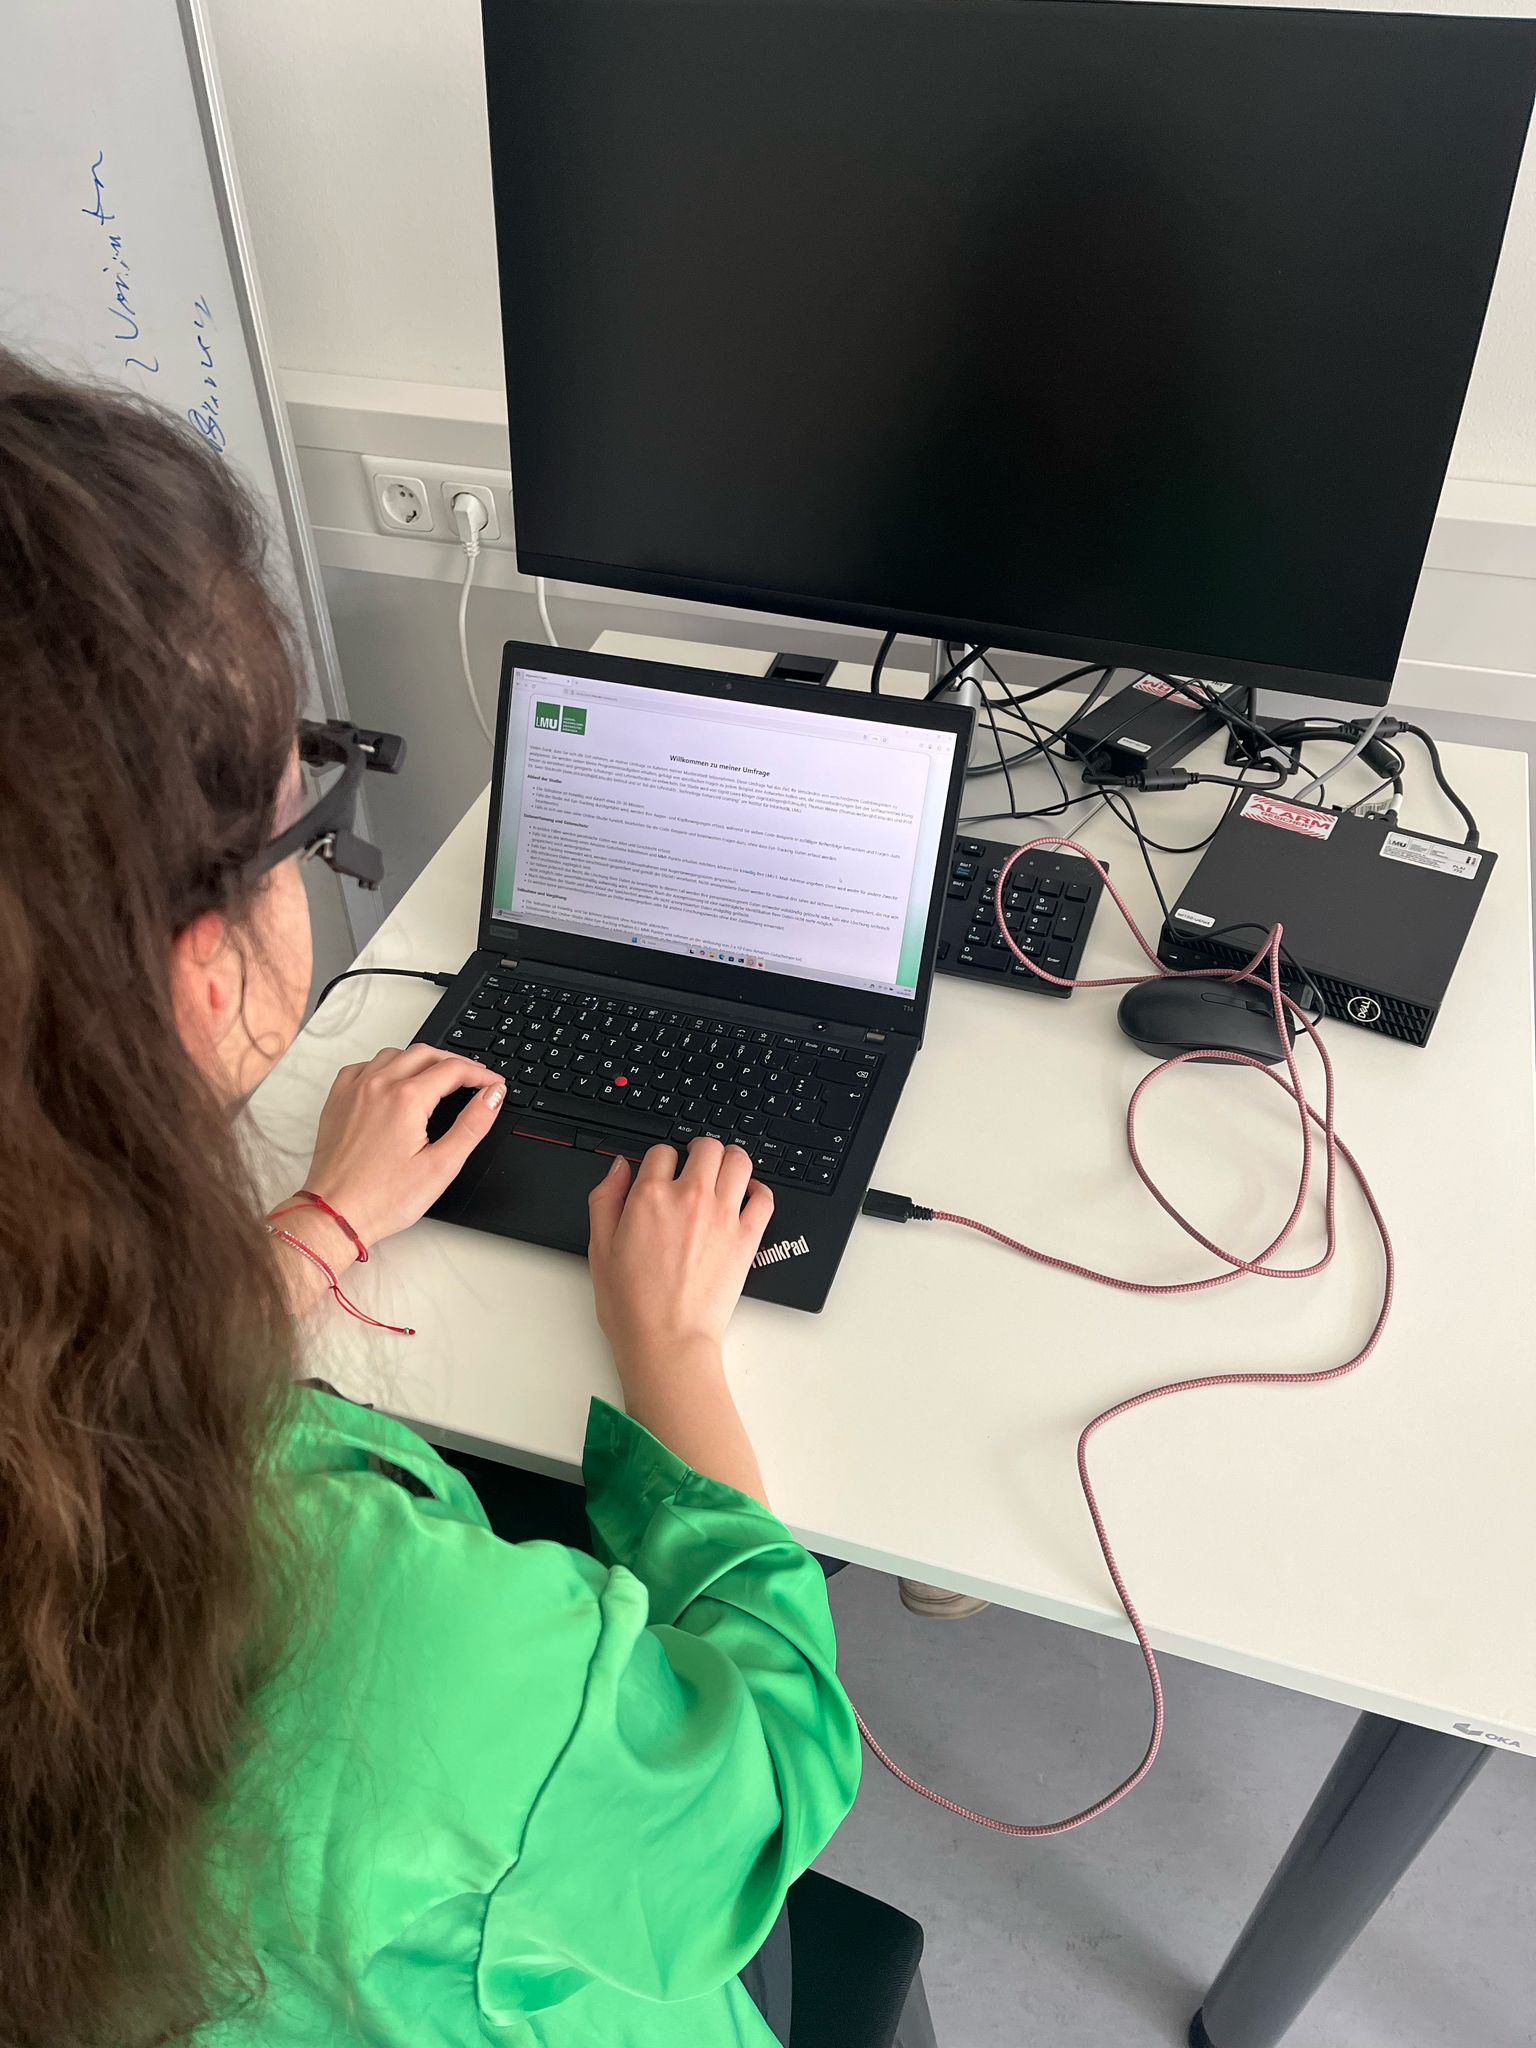
\includegraphics[scale=0.2]{figures/user.jpg}
  \caption{Participant conducting the eye-tracking study }
  \label{fig:AnhangsChor}
\end{figure}



\end{enumerate}



\subsection{Procedure for the online study without eye-tracking}


\begin{enumerate}
    \item \textbf{Introduction} Participants were informed about the purpose of the study, data collection methods, and their right to withdraw from the study at any time. Participants read all relevant information themselves and then they proceeded to the questionnaire.
    
    \item \textbf{First part of questionnaire:}
    Participants answered several questions providing demographic, background, and programming experience information. When the students filled out these questions, they proceeded to the main part of the questionnaire - code comprehension task.

    \item \textbf{Main part of questionnaire - code comprehension task:} Each participant was shown seven different code snippets. The order of the code snippets was randomized. The participants read each code snippet. After reading each code snippet, students answered five questions. These questions are related to the corresponding code snippet. Since there was no eye-tracking device, only their answers and response times were recorded.

    \item \textbf{Final part of the questionnaire:}
    The participants answered several questions providing information about their opinions on commenting and indentation in code.
\end{enumerate}




\section{Ethical considerations}

\begin{enumerate}
    \item \textbf{Informed Consent: }All participants receive clear information about the purpose of the study. The participants have the right to withdraw at any time. All information is displayed on the welcome page of the questionnaire (Figure 3.9).

\begin{figure} [H]
  \centering
  
\includegraphics[scale=0.45]{figures/welcome_page.png}
  \caption{Welcome page of the questionnaire }
  \label{fig:AnhangsChor}
\end{figure}

    
    \item \textbf{Data Protection}
    \begin{itemize}
        \item Demographic information, such as gender and age, is collected. If participants choose to receive compensation from the university, they provide their university email address. The rest of the data is anonymized and stored for a maximum of three years. Non-anonymized data is stored for a maximum of three years.
        \item  For eye-tracking participants, video recordings and gaze data are stored. For all participants, their questionnaire responses are stored. At any time, participants can request deletion of their data. No personal data is shared with third parties.
    \end{itemize}
\end{enumerate}

\chapter{Results}
This chapter presents the findings based on the collected data from the study. 

\section{Participants}

The study involved a total of 31 Bachelor’s students: 11 took part in the eye-tracking study, while the remaining 20 participated in the online study. The majority were between 18 and 25 years old (Figure 4.1).
Participants varied in their academic progress, with most being in mid to later semesters (Figure 4.2).
In terms of programming, the majority had at least some coding experience. Most reported having 1 to 2 years of experience (Figure 4.3).
As for Java knowledge, most students rated their skills as average. Only two participants reported having very good Java skills (Figure 4.4).


\begin{figure} [H]
  \centering
  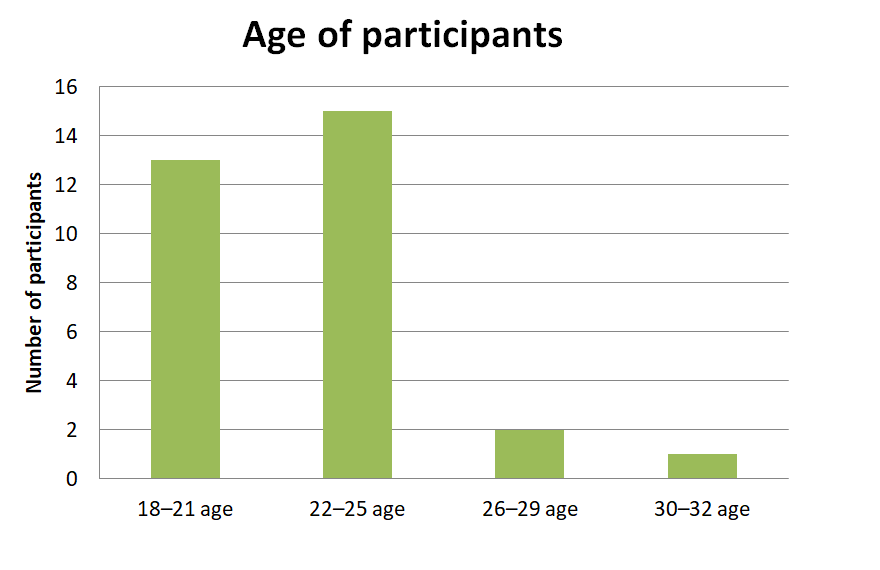
\includegraphics[scale=0.8]{figures/age.png}
  \caption{Age distribution of participants}
  \label{fig:AnhangsChor}
\end{figure}


\begin{figure} [H]
  \centering
  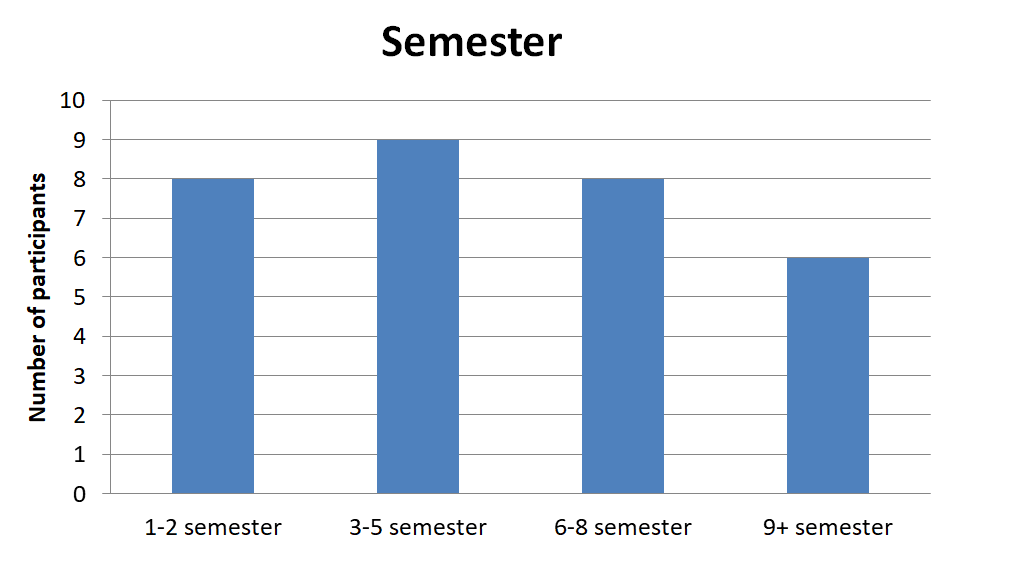
\includegraphics[scale=0.8]{figures/semester.png}
  \caption{Participants' semester}
  \label{fig:AnhangsChor}
\end{figure}

\begin{figure} [H]
  \centering
  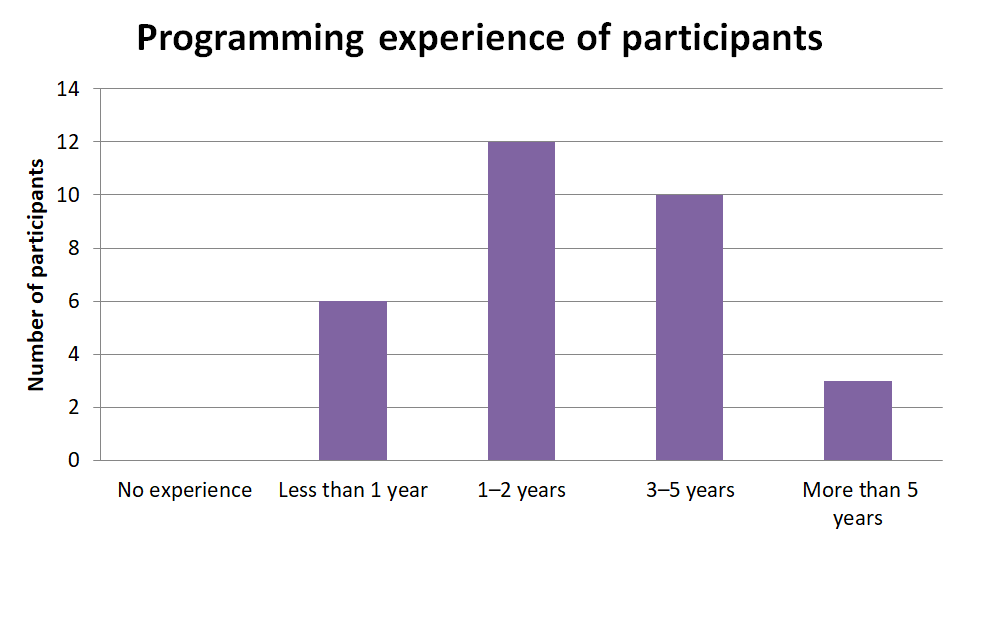
\includegraphics[scale=0.8]{figures/p_exp.png}
  \caption{Programming experience of participants}
  \label{fig:AnhangsChor}
\end{figure}


\begin{figure} [H]
  \centering
  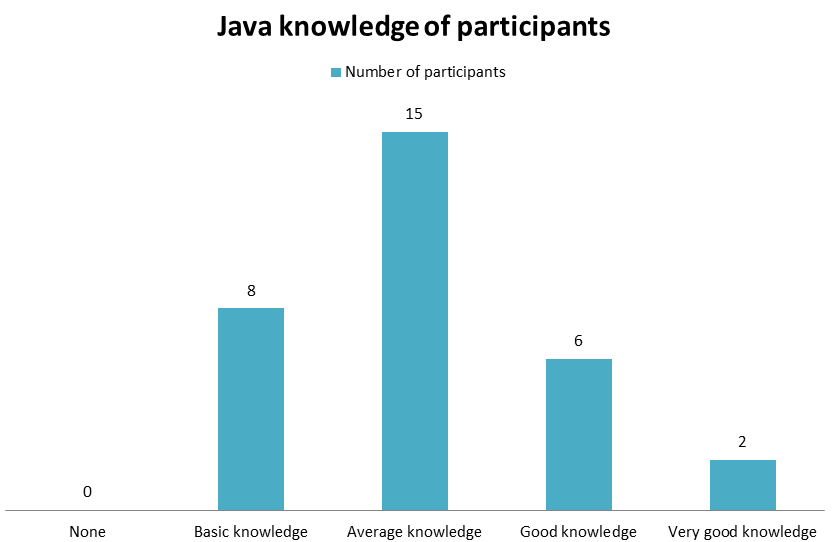
\includegraphics[scale=0.85]{figures/java_kn.png}
  \caption{Java knowledge of participants}
  \label{fig:AnhangsChor}
\end{figure}


\section{Code snippets}
Not all participants answered every question in the study. The questions related to code snippets 1, 2, and 6 were answered by 29 people; code snippets 3, 4, and 5 by 28 people, and snippet 7 by 27 people.  However, the overall response remains sufficiently balanced.

\section{Statistical analysis}

Regarding the answers for the first question of questionnaire for each code snippet, some participants gave briefly answers, while others gave more detailed ones. The difference in length could have affected the response time. Therefore, the variable Response time per code snippet was not included in the analysis. The dependent variables, such as Comprehension score, Comment quality score, and Indentation quality score, are ordinal, but do not assume equal intervals between the points.
Since the Mann-Whitney U test is suitable for this type of variables, it is used mainly in this thesis \cite{MacFarland2016}.
A significance level of \(\alpha = 0.05\) was used for all tests.

\section{Indentation}

\subsection{Indentation quality score}


Mann-Whitney U test was conducted to investigate whether 4-space indentation improves code readability compared to no indentation. The analysis was based on the Indentation quality score. The hypotheses were defined as:  H0 (Null Hypothesis): The Indentation quality score for the 4-space indented code snippet is less than or equal to that of the unindented code. H1(Alternative Hypothesis): The Indentation quality score for the 4-space indented code snippet is greater than that of the unindented code.

Figure 4.5 presents the medians for both levels of indentation. The test presented a p-value of p < .001, which is below the significance level \(\alpha\). Therefore, H0 was rejected. This result indicates that the Indentation quality score for the 4-space indented code was significantly higher than that for the unindented code. 

\begin{figure} [H]
  \centering
  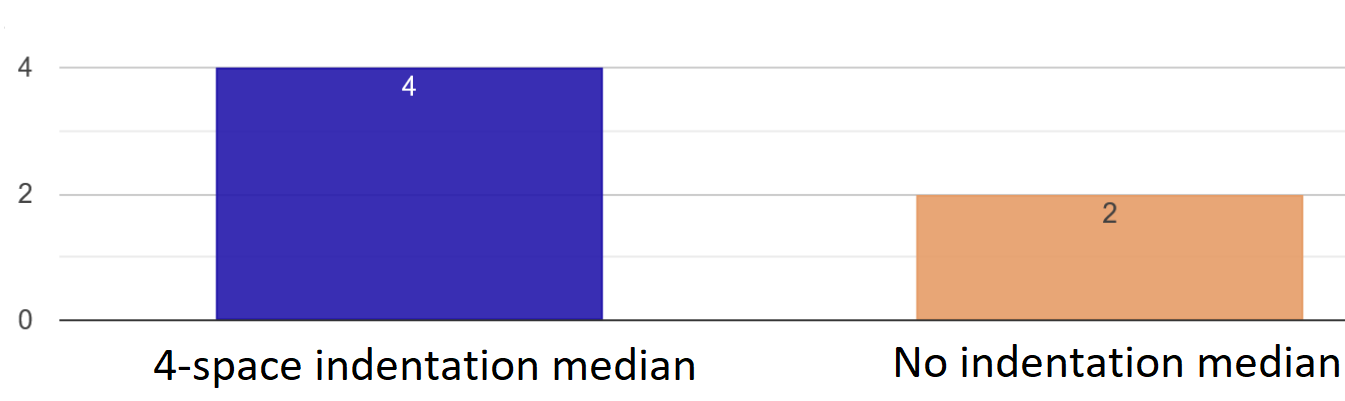
\includegraphics[scale=0.6]{figures/4-0-q5png.png}
  \caption{Indentation quality score: 4-space indentation median and No indentation median}
  \label{fig:AnhangsChor}
\end{figure}


Another Mann-Whitney U test was conducted to investigate whether 4-space indentation improves code readability compared to random indentation. The analysis was based on the Indentation quality score. The hypotheses were defined as:  H0 (Null Hypothesis): The Indentation quality score for the 4-space indented code snippet is less than or equal to that of the randomly indented code. H1 (Alternative Hypothesis): The Indentation quality score for the 4-space indented code snippet is greater than that of the randomly indented code.


Figure 4.6 displays the medians for both levels of indentation. 
The test produced a p-value of p = .001, which is below the significance level \(\alpha\). Therefore, H0 was rejected. The result presented that the Indentation quality score for the 4-space indented code was significantly higher than for the randomly indented code.

\begin{figure} [H]
  \centering
  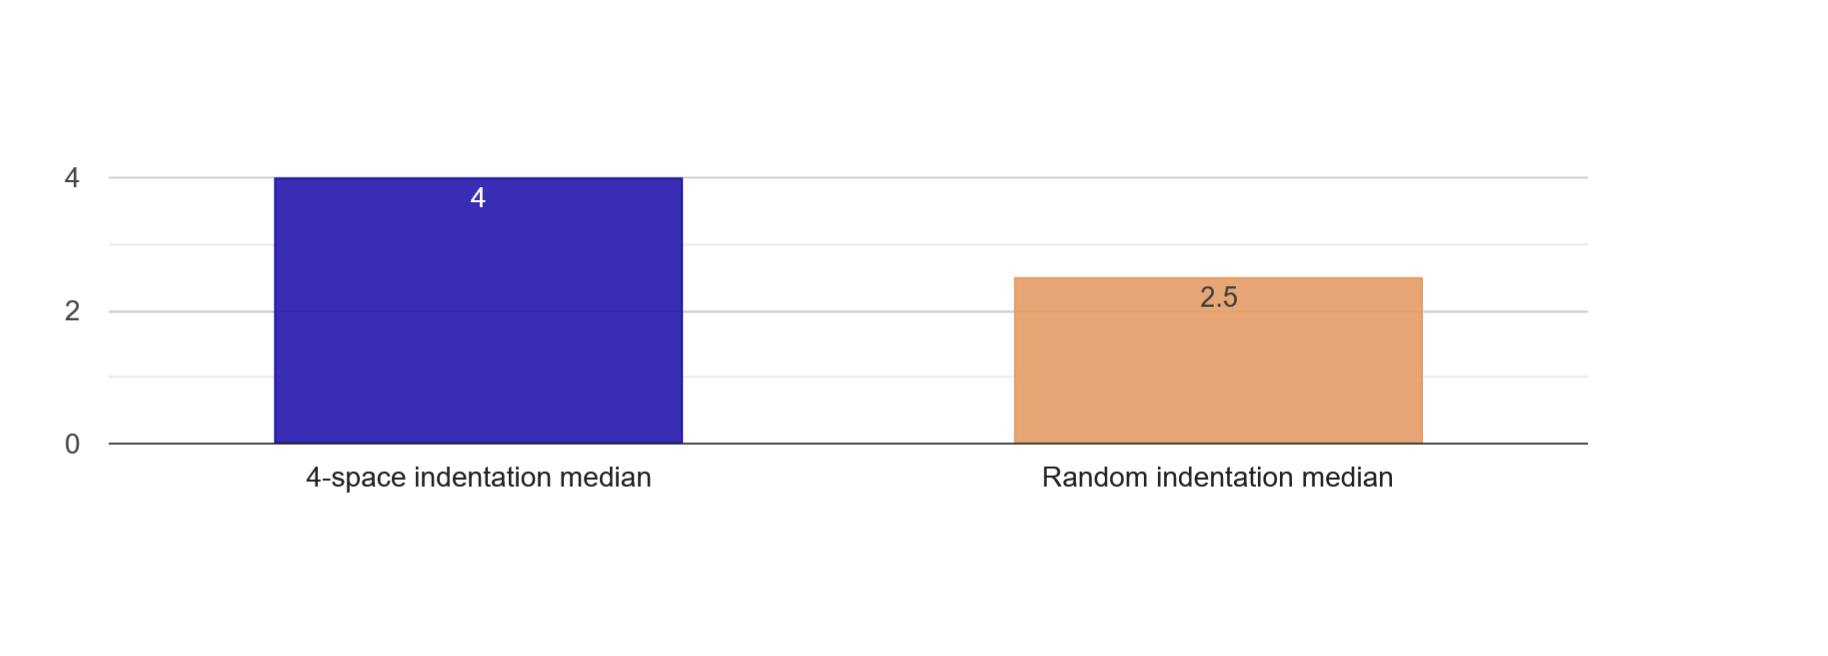
\includegraphics[scale=0.58]{figures/4-r-q5.png}
  \caption{Indentation quality score: 4-space indentation median and Random indentation median}
  \label{fig:AnhangsChor}
\end{figure}


Another  U test was performed to investigate whether random indentation improves the readability of code compared to code with no indentation. The analysis was based on the Indentation quality score. The hypotheses were defined as:  H0 (Null Hypothesis): The Indentation quality score for the randomly indented code snippet is less than or equal to that of the code snippet with no indentation.  H1(Alternative Hypothesis): The Indentation quality score for the randomly indented code snippet is greater than that of the code snippet with no indentation.


\begin{figure} [H]
  \centering
  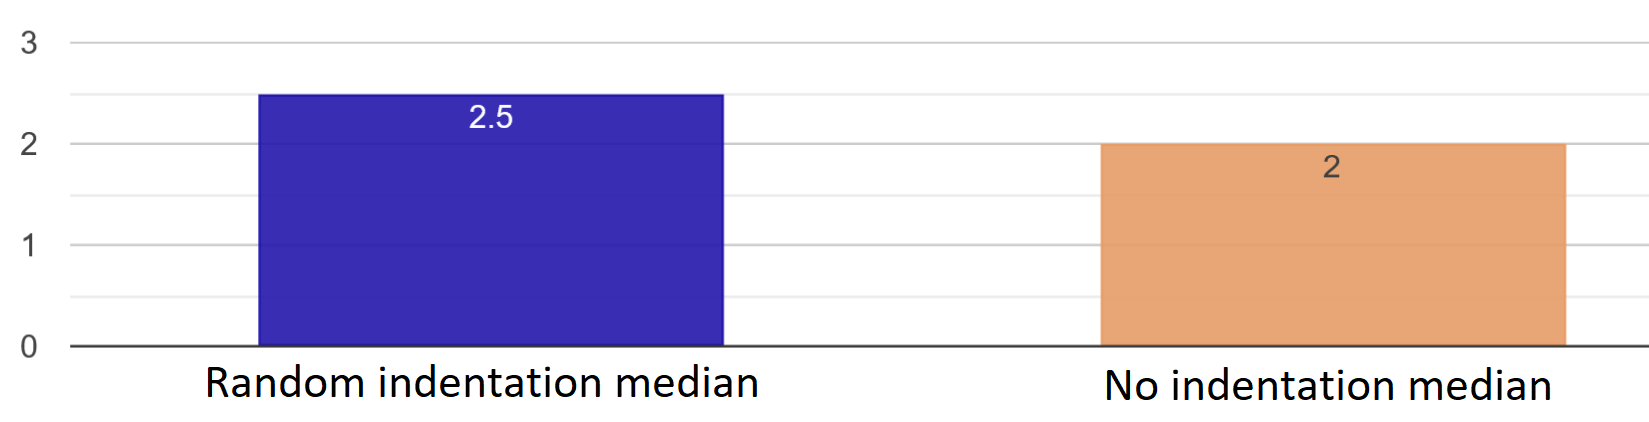
\includegraphics[scale=0.49]{figures/r-0-q5.png}
  \caption{Indentation quality score: Random indentation median and No indentation median}
  \label{fig:AnhangsChor}
\end{figure}

Figure 4.7 visualizes the medians for both levels of indentation. 
The test presented a p-value of  p = .021, which is less than the significance level \(\alpha \). Therefore, the H0 was rejected. The result reveals that the Indentation quality score for the randomly indented code was significantly higher than that of the unindented code.

Figure 4.8 shows an overview of the median scores for each indentation level with respect to the Indentation quality score. The highest median score has the 4-space indentation, followed by random indentation and no indentation.

\begin{figure} [H]
  \centering
  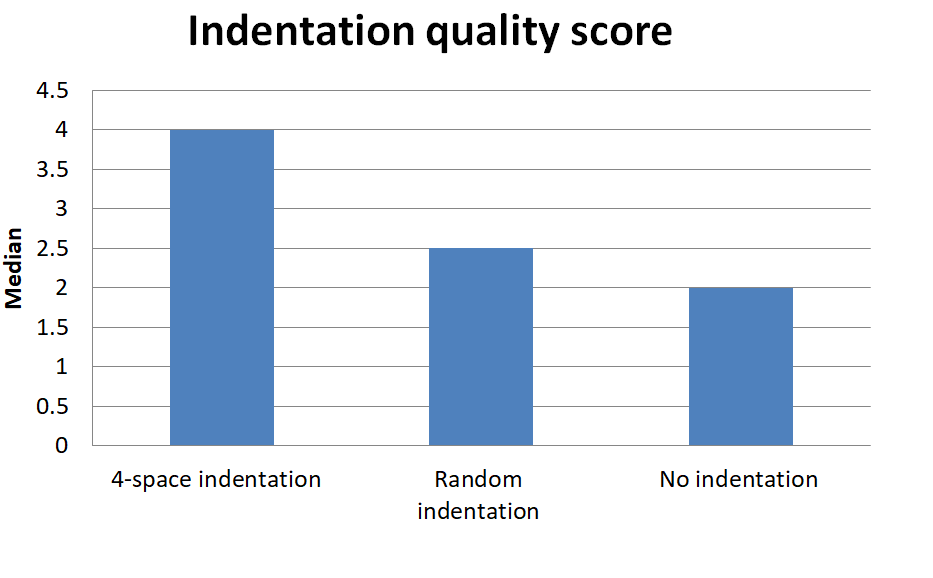
\includegraphics[scale=0.96]{figures/indsM.png}
  \caption{Indentation quality score: medians}
  \label{fig:AnhangsChor}
\end{figure}


\subsection{Comprehension score}
Another Mann-Whitney U test was conducted to investigate whether random indentation enhance the comprehension  of code compared to code with no indentation. The analysis was based on the Comprehension score. The hypotheses were defined as: H0 (Null Hypothesis): The Comprehension score for the code snippet with no indentation is equal to that of the randomly indented code snippet. H1 (Alternative Hypothesis): The Comprehension score for the code snippet with no indentation is not equal to that of the randomly indented code snippet. Figure 4.9 displays the medians for both levels of indentation.



\begin{figure} [H]
  \centering
  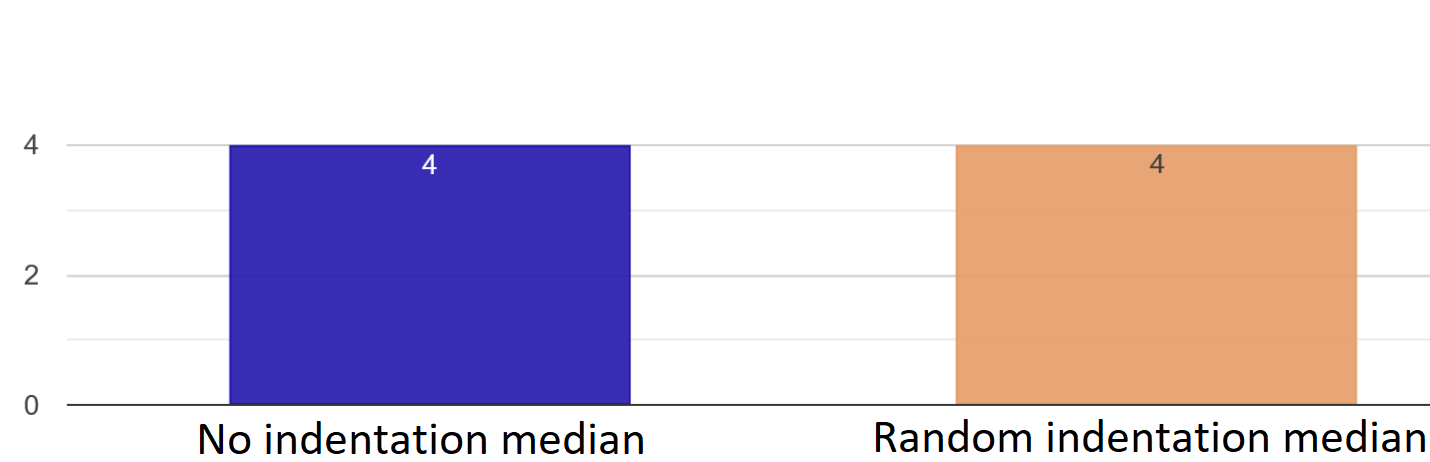
\includegraphics[scale=0.55]{figures/0-r-q3.png}
  \caption{Comprehension score:  No indentation median and Random indentation median}
  \label{fig:AnhangsChor}
\end{figure}

The test produced a p-value of p = .129, which is greater than the significance level \(\alpha\). Therefore, H0 cannot be rejected. This result indicates that the difference in Comprehension score between the randomly indented and unindented code snippets was not statistically significant.


\subsection{Confidence rating}

Another Mann-Whitney U test was conducted to investigate whether random indentation improves the code confidence rating compared to code with no indentation. The analysis was based on the Confidence rating, a dependent variable derived from participant responses. The hypotheses were defined as: H0 (Null Hypothesis): The Confidence rating for the code snippet with no indentation is equal to that of the randomly indented code snippet. H1 (Alternative Hypothesis): The Confidence rating for the code snippet with no indentation is not equal to that of the randomly indented code snippet.
The test produced a p-value of p = .609, which is greater than the significance level \(\alpha\). Therefore, H0 cannot be rejected. This result reveals that the difference in Confidence rating between the randomly indented and unindented code snippets was not statistically significant.  



Table 4.1 presents an overview of all hypotheses related to the different levels of indentation, with respect to Indentation quality score, Comprehension score, and Confidence rating.

\begin{table}[ht]
\centering
\small
\begin{tabular}{|p{5cm}|p{6cm}|p{2.5cm}|}
\hline
\rule{0pt}{1.2em}\textbf{Variable} & \textbf{Hypothesis (H0)} & \textbf{H0 Rejected?} \\[0.5em]
\hline
\rule{0pt}{1.2em}Indentation quality score & 4-space $\leq$ No indentation & Rejected \\[0.5em]
\hline
\rule{0pt}{1.2em}Indentation quality score & 4-space $\leq$ Random indentation & Rejected \\[0.5em]
\hline
\rule{0pt}{1.2em}Indentation quality score & Random $\leq$ No indentation & Rejected \\[0.5em]
\hline
\rule{0pt}{1.2em}Comprehension score & Random = No indentation & Not rejected \\[0.5em]
\hline
\rule{0pt}{1.2em}Confidence rating & Random = No indentation & Not rejected \\[0.5em]
\hline
\end{tabular}
\caption{Hypotheses related to indentation levels}
\end{table}


\subsection{Indentation methods}
When participants were asked how they handle code indentation, several answers were selected. Figure 4.9 shows that most participants use the Tab key. Only a few students use automatic tools.  

\begin{figure} [H]
  \centering
  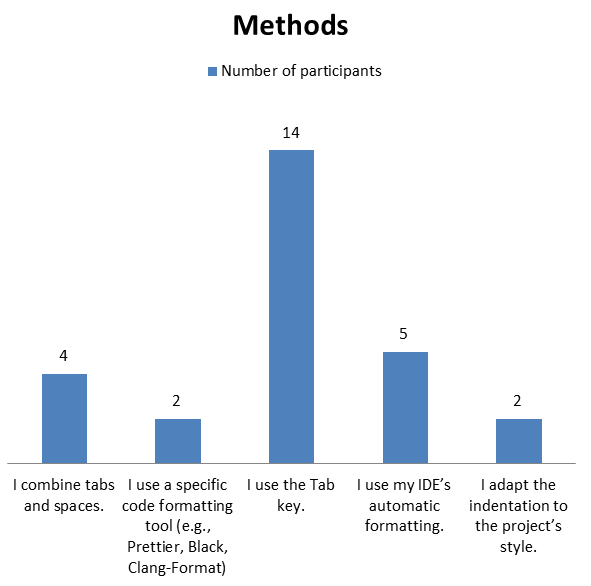
\includegraphics[scale=0.8]{figures/inM.png}
  \caption{Methods for code indentation}
  \label{fig:AnhangsChor}
\end{figure}



\section{Comments}

\subsection{Comment quality score}

To explore whether helpful comments improve the comment quality of the code compared to no comments, a Mann-Whitney U test was conducted.  The analysis was based on the Comment quality score. The hypotheses were defined as: H0 (Null Hypothesis): The Comment quality score for the code snippet with helpful comments is less than or equal to that of the code with no comments.  H1 (Alternative Hypothesis): The Comment quality score for the code snippet with helpful comments is greater than that of the code with no comments.

Figure 4.11 shows the medians for both comment formats.
The test produced a p-value of p < .001, which is below the significance level $\alpha$. Therefore, H0 was rejected. This result reveals that the Comment quality score for the code with helpful comments was significantly higher than that for the code with no comments.

\begin{figure} [H]
  \centering
  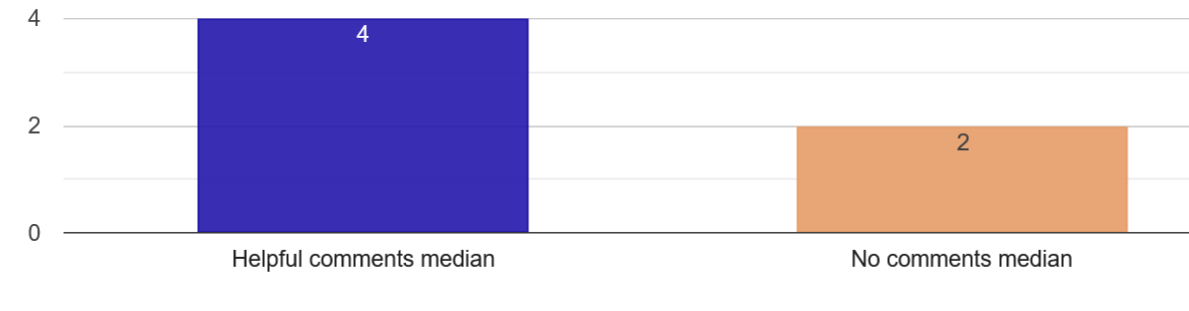
\includegraphics[scale=0.6]{figures/h-0-q4.png}
  \caption{Comment quality score: Helpful comments median and No comments median}
  \label{fig:AnhangsChor}
\end{figure}


A Mann-Whitney U test was performed to investigate whether helpful comments improve the comment quality of the code compared to minimal comments. The analysis was based on the Comment quality score. The hypotheses were defined as: H0 (Null Hypothesis): The Comment quality score for the code snippet with helpful comments is less than or equal to that of the code with minimal comments.  H1 (Alternative Hypothesis): The Comment quality score for the code snippet with helpful comments is greater than that of the code with minimal comments. The test resulted in a p-value of p = .024, which is below the significance level $\alpha $. Therefore, H0 was rejected. This result reveals that the Comment quality score for the code with helpful comments was significantly higher than that for the code with minimal comments.





To explore whether helpful comments enhance the comment quality of the code compared to redundant comments, a  U test was conducted.  The analysis was based on the Comment quality score. The hypotheses were defined as: H0 (Null Hypothesis): The Comment quality score for the code snippet with helpful comments is less than or equal to that of the code with redundant comments.  H1 (Alternative Hypothesis): The Comment quality score for the code snippet with helpful comments is greater than that of the code with redundant comments. The test produced a p-value of p = .022, which is below the significance level $\alpha $. Therefore, H0 was rejected. This result reveals that the Comment quality score for the code with helpful comments was significantly higher than that for the code with redundant comments. 



A Mann-Whitney U test was conducted to investigate whether minimal comments have an impact on the comment quality of the code compared to redundant comments. The analysis was based on the Comment quality score. The hypotheses were defined as: H0 (Null Hypothesis): The Comment quality score for the code snippet with minimal comments is equal to that of the code snippet with redundant comments. H1 (Alternative Hypothesis): The Comment quality score for the code snippet with minimal comments is not equal to that of the code snippet with redundant comments.  The test produced a p-value of p =.644, which is greater than the significance level $\alpha$. Therefore, H0 cannot be rejected. This result reveals that the difference in Comment quality score between minimal comments code snippet and the redundant comments code snippet populations is not big enough to be statistically significant.


\subsection{Comprehension score}
A U test was conducted to explore whether code snippet with helpful comments improves code comprehension compared to code with no comments. The analysis was based on the Comprehension score. The hypotheses were defined as: H0 (Null Hypothesis): The Comprehension score for the code snippet with helpful comments is less than or equal to that of the code with no comments.  H1 (Alternative Hypothesis): The Comprehension score for the code snippet with helpful comments is greater than that of the code with no comments.


Figure 4.12 presents the medians for both comments formats.
The test produced a p-value of  p < .001, which is below the significance level $\alpha $. Therefore, H0 was rejected.  This result reveals that the Comprehension score for the code with helpful comments was significantly higher than that for the code with no comments. 


\begin{figure} [H]
  \centering
  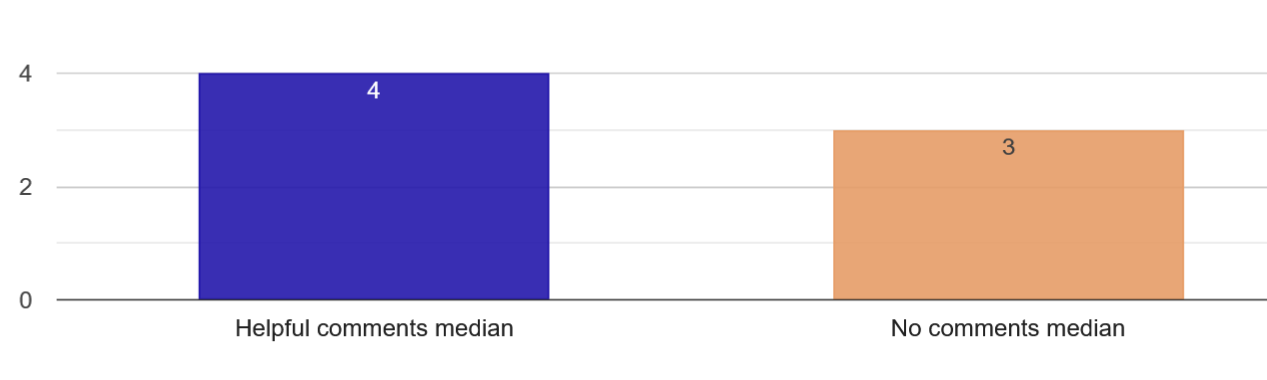
\includegraphics[scale=0.6]{figures/h-0-q3.png}
  \caption{Comprehension score:  Helpful comments median and No comments median}
  \label{fig:AnhangsChor}
\end{figure}




A U test was performed to investigate whether code snippet with helpful comments improves code comprehension compared to code with minimal comments. The analysis was based on the Comprehension score. The hypotheses were defined as: H0 (Null Hypothesis): The Comprehension score for the code snippet with helpful comments is less than or equal to that of the code with minimal comments.  H1 (Alternative Hypothesis): The Comprehension score for the code snippet with helpful comments is greater than that of the code with minimal comments.

Figure 4.13 displays the medians for both comments formats.
The test indicates a p-value of p < .001, which is below the significance level $\alpha$. Therefore, H0 was rejected.  This test reveals that the Comprehension score for the code with helpful comments was significantly higher than that for the code with minimal comments. 

\begin{figure} [H]
  \centering
  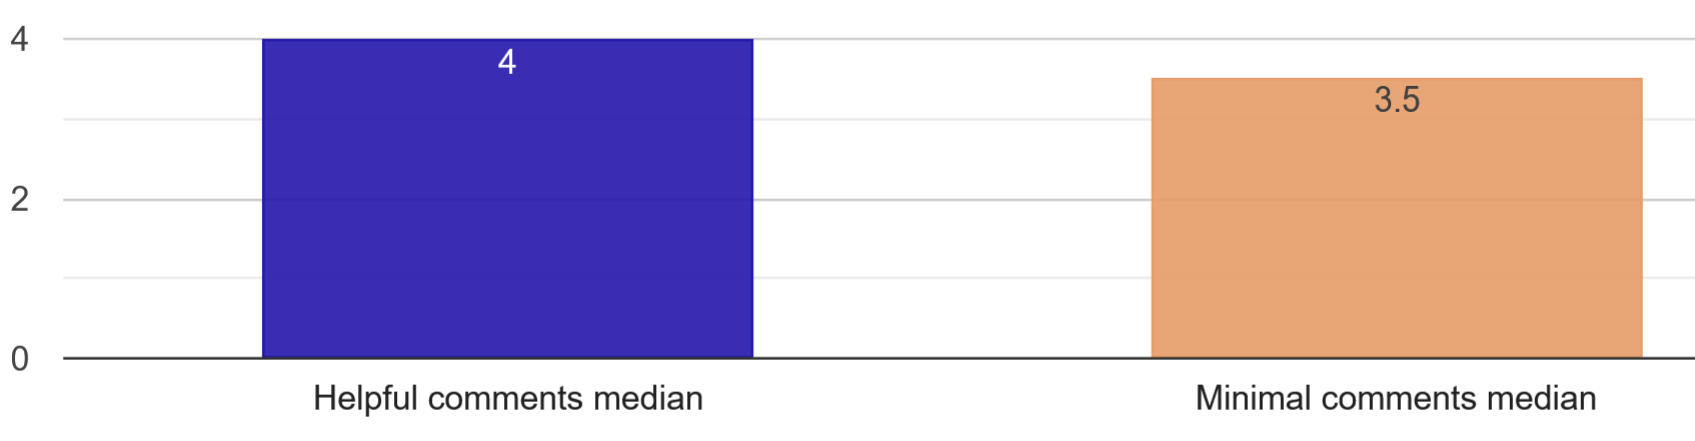
\includegraphics[scale=0.43]{figures/h-m-q3.png}
  \caption{Comprehension score:  Helpful comments median and Minimal comments median}
  \label{fig:AnhangsChor}
\end{figure}


A U test was conducted to investigate whether code snippet with redundant comments enhance code comprehension compared to code with minimal comments. The analysis was based on the Comprehension score. The hypotheses were defined as: H0 (Null Hypothesis): The Comprehension score for the code snippet with redundant comments is less than or equal to that of the code with minimal comments.  H1 (Alternative Hypothesis): The Comprehension score for the code snippet with redundant comments is greater than that of the code with minimal comments. 


Figure 4.14 displays the medians for both comments formats.
The test indicates a p-value of p = .007, which is below the significance level $\alpha $. Therefore, H0 can be rejected.  This test reveals that the Comprehension score for the code with redundant comments was significantly higher than that for the code with minimal comments. 

\begin{figure} [H]
  \centering
  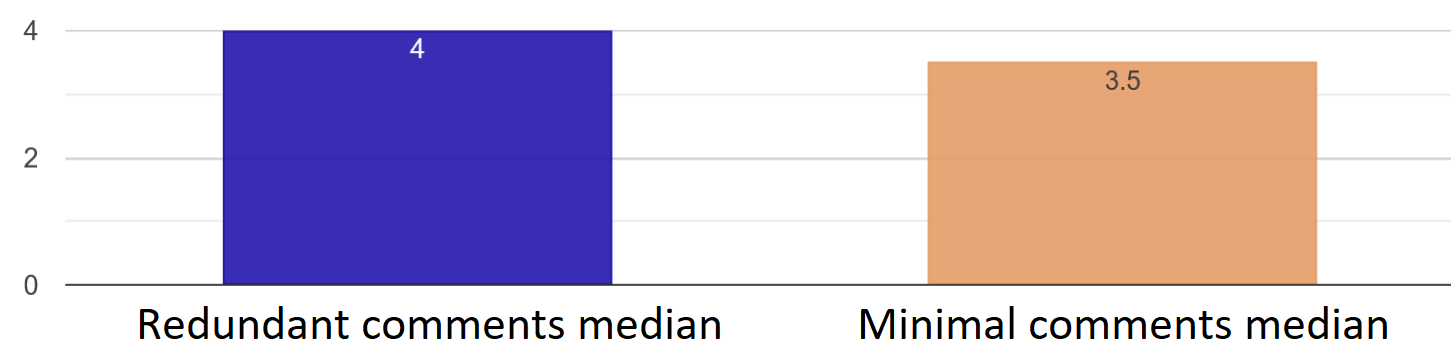
\includegraphics[scale=0.56]{figures/red-min-q3.png}
  \caption{Comprehension score:  Redundant comments median and Minimal comments median}
  \label{fig:AnhangsChor}
\end{figure}


Figure 4.15 illustrates the median comprehension scores in the commenting formats: helpful, redundant, minimal, and without comments.

\begin{figure} [H]
  \centering
  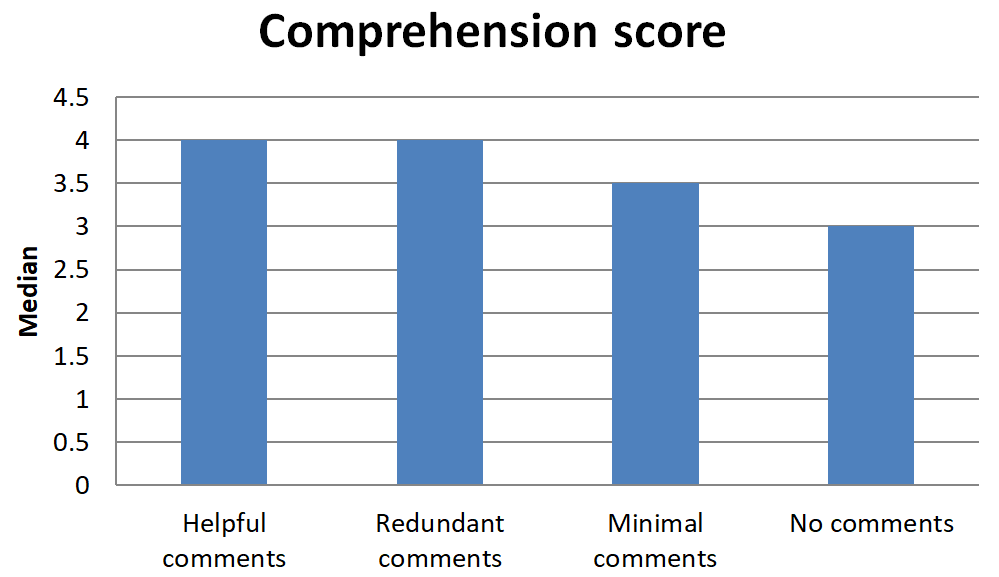
\includegraphics[scale=0.8]{figures/comMed.png}
  \caption{Comprehension score: medians}
  \label{fig:AnhangsChor}
\end{figure}



\subsection{Confidence rating}
A U test was performed to investigate whether code snippet with helpful comments enhance code confidence compared to code with no comments. The analysis was based on the Confidence rating. The hypotheses were defined as:  H0 (Null Hypothesis): The Confidence rating for the code snippet with helpful comments is less than or equal to that of the code with no comments.  H1 (Alternative Hypothesis): The Confidence rating for the code snippet with helpful comments is greater than that of the code with no comments. The test produced a p-value of   p < .001, which is below the significance level $\alpha$. Therefore, H0 was rejected.  This result reveals that the Confidence rating  for the code with helpful comments was significantly higher than that for the code with no comments. 



A test was conducted to investigate whether code snippet with helpful comments improves code confidence compared to code with minimal comments. The analysis was based on the Confidence rating. The hypotheses were defined as:  H0 (Null Hypothesis): The Confidence rating for the code snippet with helpful comments is less than or equal to that of the code with minimal comments.  H1 (Alternative Hypothesis): The Confidence rating for the code snippet with helpful comments is greater than that of the code with minimal comments. The test produced a p-value of   p < .001, which is below the significance level $\alpha$. Therefore, H0 was rejected.  This result reveals that the Confidence rating  for the code with helpful comments was significantly higher than that for the code with minimal comments.  


To investigate whether code snippet with redundant comments improves code confidence compared to code with minimal comments, a U test was performed. The analysis was based on the Confidence rating. The hypotheses were defined as:  H0 (Null Hypothesis): The Confidence rating for the code snippet with redundant comments is less than or equal to that of the code with minimal comments.  H1 (Alternative Hypothesis): The Confidence rating for the code snippet with redundant comments is greater than that of the code with minimal comments.      
The test produced a p-value of  p = .006, which is below the significance level $\alpha $. Therefore, H0 was rejected.  This result suggests that the Confidence rating  for the code with redundant comments was significantly higher than that for the code with minimal comments.   


A U test was performed to investigate whether code snippet with redundant comments improves code confidence compared to code without comments. The analysis was based on the Confidence rating. The hypotheses were defined as:  H0 (Null Hypothesis): The Confidence rating for the code snippet with redundant comments is less than or equal to that of the code without comments.  H1 (Alternative Hypothesis): The Confidence rating for the code snippet with redundant comments is greater than that of the code without comments.      
The test produced a p-value of  p = .011, which is below the significance level $\alpha $. Therefore, H0 was rejected.  This result suggests that the Confidence rating  for the code with redundant comments was significantly higher than that for the code without comments.   Table 4.2 presents an overview of all hypotheses related to the comment formats.

\begin{table}[ht]
\centering
\small
\begin{tabular}{|p{4cm}|p{6cm}|p{2.5cm}|}
\hline
\rule{0pt}{1.2em}\textbf{Variable} & \textbf{Hypothesis (H0)} & \textbf{H0 Rejected?} \\[0.5em]
\hline
\rule{0pt}{1.2em}Comment quality score & Helpful $\leq$ No comments & Rejected \\[0.5em]
\hline
\rule{0pt}{1.2em}Comment quality score & Helpful $\leq$ Minimal comments & Rejected \\[0.5em]
\hline
\rule{0pt}{1.2em}Comment quality score & Helpful $\leq$ Redundant comments & Rejected \\[0.5em]
\hline
\rule{0pt}{1.2em}Comment quality score & Minimal = Redundant comments & Not rejected \\[0.5em]
\hline
\rule{0pt}{1.2em}Comprehension score & Helpful $\leq$ No comments & Rejected \\[0.5em]
\hline
\rule{0pt}{1.2em}Comprehension score & Helpful $\leq$ Minimal comments & Rejected \\[0.5em]
\hline
\rule{0pt}{1.2em}Comprehension score & Redundant $\leq$ Minimal comments & Rejected \\[0.5em]
\hline
\rule{0pt}{1.2em}Confidence rating & Helpful $\leq$ No comments & Rejected \\[0.5em]
\hline
\rule{0pt}{1.2em}Confidence rating & Helpful $\leq$ Minimal comments & Rejected \\[0.5em]
\hline
\rule{0pt}{1.2em}Confidence rating & Redundant $\leq$ Minimal comments & Rejected \\[0.5em]
\hline
\rule{0pt}{1.2em}Confidence rating & Redundant $\leq$ No comments & Rejected \\[0.5em]
\hline
\end{tabular}
\caption{Hypotheses related to the comment formats}
\end{table}



\subsection{Quality of comments}


When participants were asked what characterizes well-commented code for them, their responses indicated common opinions. They think comments should explain what the code does. Participant E thought that the code snippet that has "direct and clearly written comments", is well-commented. Participants generally agree on what makes code badly commented. They think it is problematic when comments are missing. Another issue is over-commenting, where every single line is explained. Participant A thought that comments which are "unclear, repeat the program code, and no longer reflect the current state of the code" are bad. When participants were asked how often they follow their own guidelines when writing code comments, most participants answered that they do so sometimes. Figure 4.16 shows the results.

\begin{figure} [H]
  \centering
  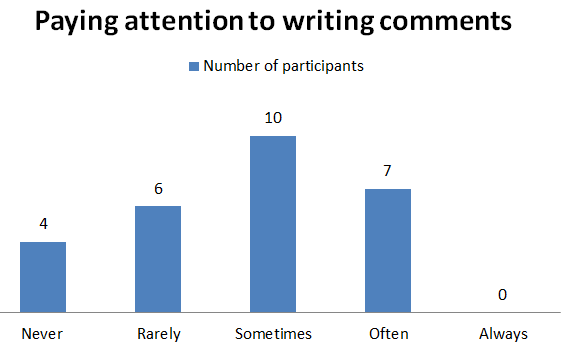
\includegraphics[scale=0.9]{figures/comAt.png}
  \caption{Paying attention to writing comments }
  \label{fig:AnhangsChor}
\end{figure}


\section{Eye-tracking results}
One common issue in the eye-tracking study was missing data caused by head movements or calibration errors. As a result, several gaze recordings were excluded from the analysis. Only eight recordings were considered. However, some of these did not provide clear results. Therefore, only five recordings were fully analyzed. 
Due to the incomplete and small dataset, a qualitative approach was applied to analyze gaze patterns: reading order and attention focus were analyzed using scanpaths and heatmaps.  
 


\subsection{Effects of indentation levels on gaze behavior}
In all three code snippets with different levels of indentation, a single AOI category was defined: keywords, including terms such as “if” and “else”. In the code snippet without indentation, three participants tended to look at these keywords and often returned to previous lines. Moreover, they showed long fixation durations.  Figure 4.17 presents a scanpath from participant A, who spent a lot of time looking at the code and returned to previous lines. 

\begin{figure} [H]
  \centering
  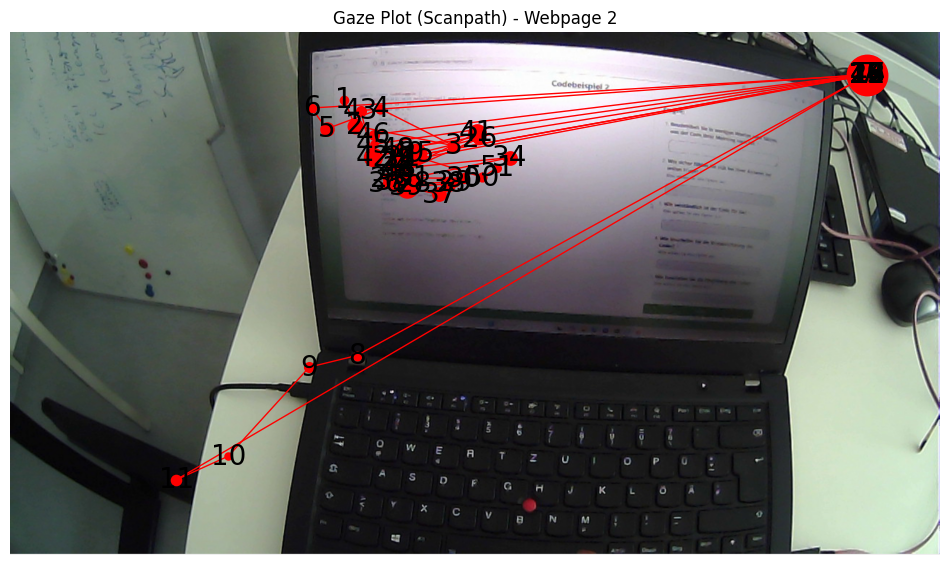
\includegraphics[scale=0.6]{figures/0-ind-rechner.png}
  \caption{Scanpath of participant A for code snippet without indentation }
  \label{fig:AnhangsChor}
\end{figure}


\begin{figure} [H]
  \centering
  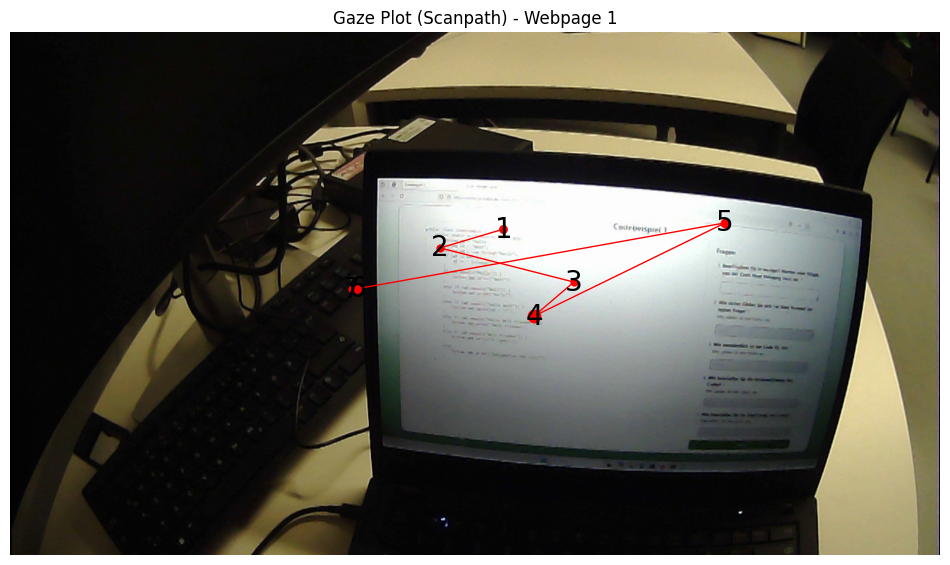
\includegraphics[scale=0.6]{figures/4-ind.png}
  \caption{Scanpath of participant B for code snippet with 4-space indentation}
  \label{fig:AnhangsChor}
\end{figure}

In the code snippet with 4-space indentation, three participants tended to follow a clear reading path. Moreover, fixation durations on keywords were notably shorter. Figure 4.18 presents a scanpath for participant B, who looked at the code lines from top to bottom without returning to previous lines.  


In the code snippet with random indentation, three participants often had long fixation durations on the keywords. Moreover, they often read the code with many jumps between lines and with inconsistent gaze directions. For instance, Figure 4.19 presents a scanpath for participant C who followed a “zig-zag” pattern — shifting his eyes inconsistently from left to right and back again.  



 



\begin{figure} [H]
  \centering
  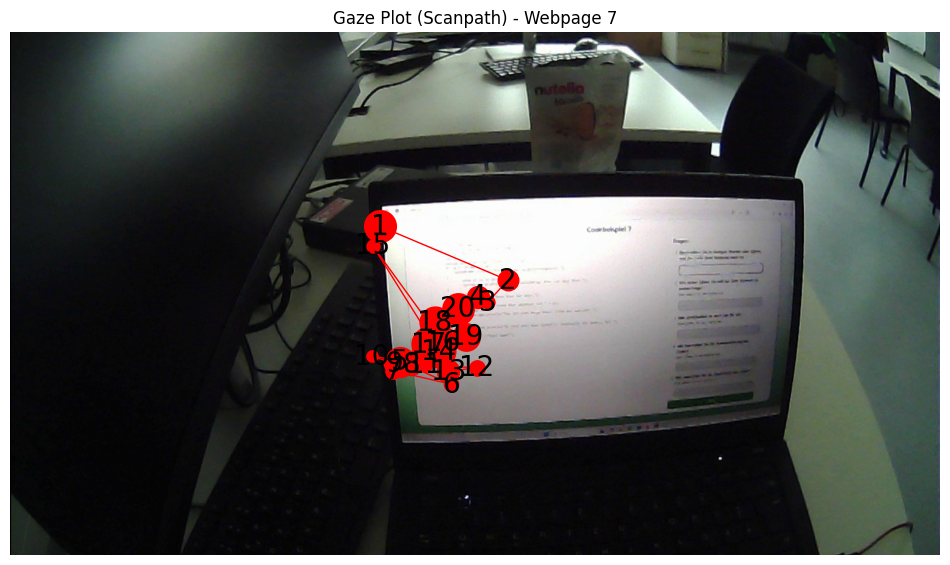
\includegraphics[scale=0.6]{figures/r-ind.png}
  \caption{Scanpath of  participant C for code snippet with random indentation}
  \label{fig:AnhangsChor}
\end{figure}



\subsection{Effects of commenting formats on gaze behavior}

In all four code snippets with different commenting formats, a single AOI category was defined: Comments. This AOI was used to investigate participants’ visual engagement with different types of comments. 

In the code snippet with helpful comments, three participants often looked at the comments before reading the code itself.  Figure 4.20 presents a scanpath from participant D whose attention at the beginning was more on the comments. In the code snippet with minimal comments, three participants tended to follow a clear reading path.  Furthermore, they did not spend much time on the comments. Figure 4.21  presents a gaze plot of participant B, indicating a short fixation duration on comments. 


In the code snippet with redundant comments, three participants tended not to spend much time on the comments or even ignored them. Figure 4.22  shows a gaze plot of participant D, whose attention was more on the code itself and not on the comments. Regarding the order of reading, some participants followed a clear reading path while others read the code in a more inconsistent order.  In the code snippet with no comments, the comment AOI was absent and participants spent more time on code lines. Figure 4.23 presents a gaze plot of participant C, indicating a long fixation duration on code lines.    Regarding the order of reading, the majority of participants followed an unclear reading path.

\begin{figure} [H]
  \centering
  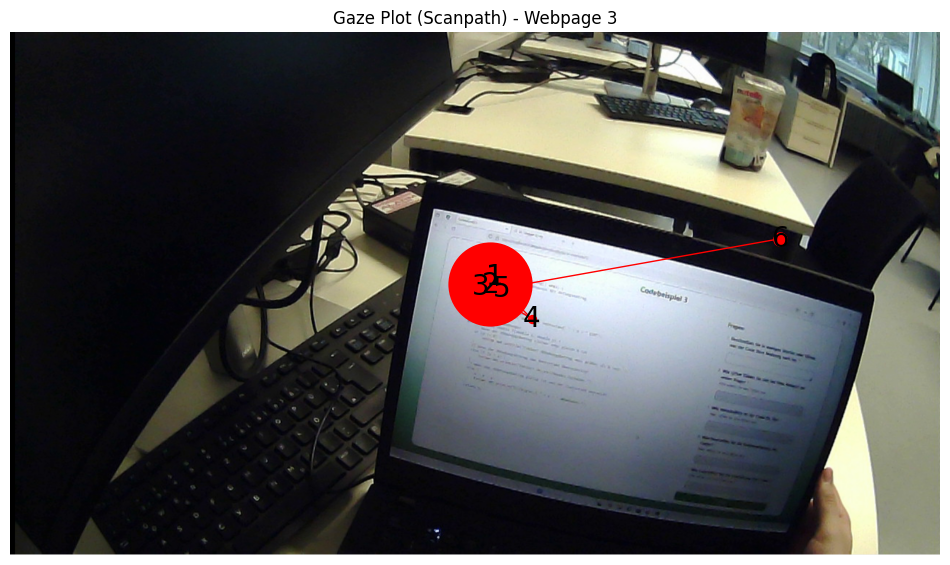
\includegraphics[scale=0.6]{figures/h-com.png}
  \caption{Scanpath of participant D for code snippet with helpful comments }
  \label{fig:AnhangsChor}
\end{figure}

\begin{figure} [H]
  \centering
  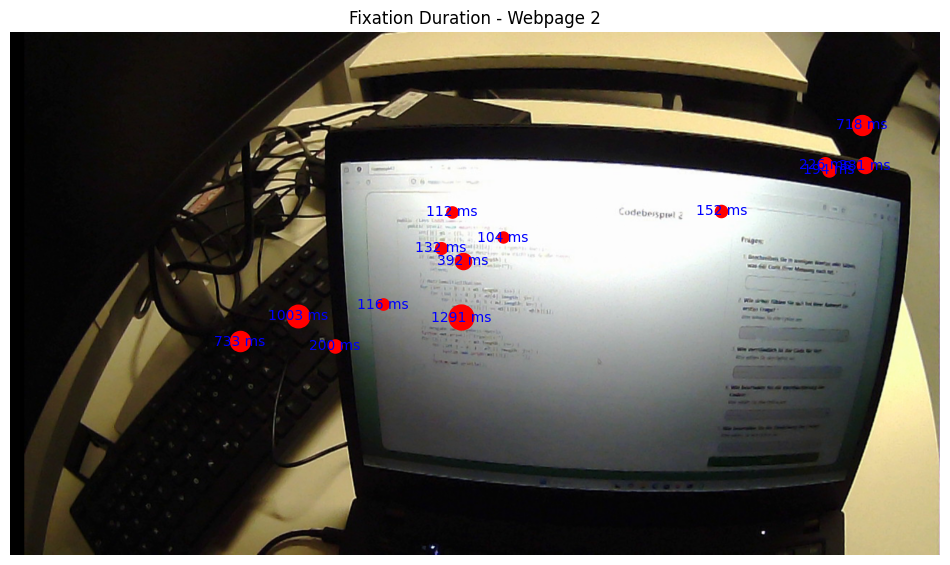
\includegraphics[scale=0.6]{figures/min-com.png}
  \caption{Fixation duration of participant B for code snippet with minimal comments}
  \label{fig:AnhangsChor}
\end{figure}

\begin{figure} [H]
  \centering
  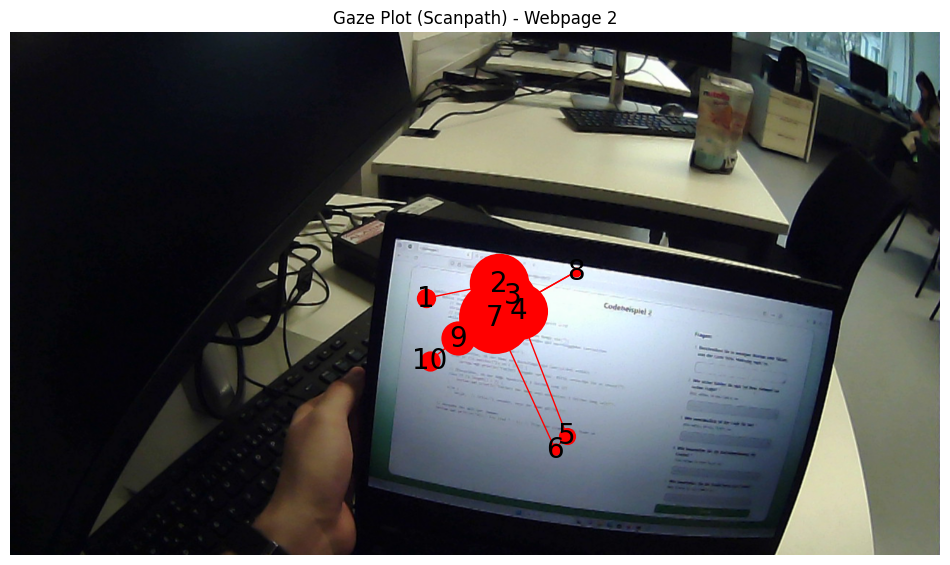
\includegraphics[scale=0.6]{figures/redun-com.png}
  \caption{Scanpath of  participant D for code snippet with redundant comments}
  \label{fig:AnhangsChor}
\end{figure}


\begin{figure} [H]
  \centering
  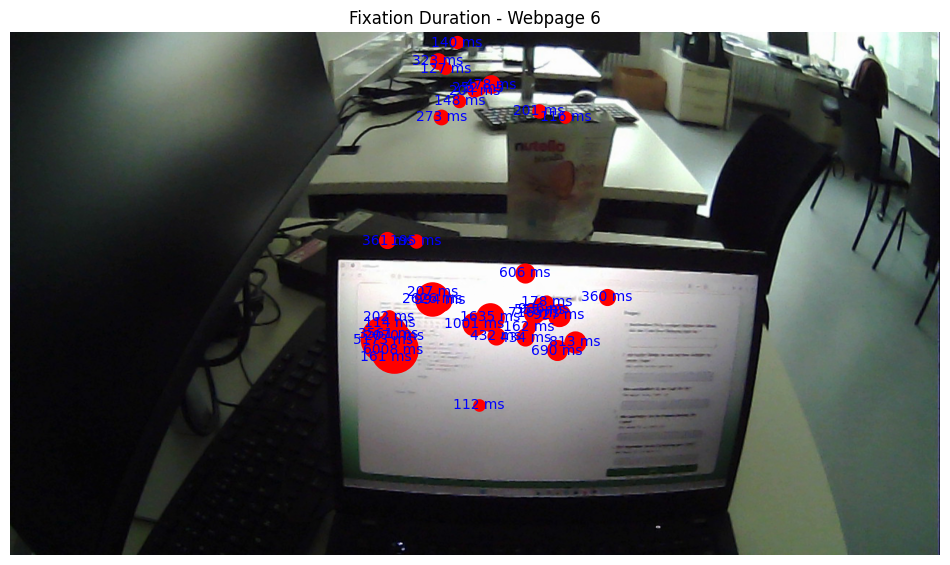
\includegraphics[scale=0.6]{figures/0-com.png}
  \caption{Fixation duration of  participant C for code snippet without comments}
  \label{fig:AnhangsChor}
\end{figure}





\chapter{Discussion}
This section discusses the findings of the study. It also presents the limitations and suggestions for improvements.


\section{Effects of indentation} 
The results present that indentation significantly affects code readability. The 4-space indentation code snippet was rated significantly better than the randomly indented snippet and the not indented snippet. This level of indentation is considered to provide a more organized structure, making the code easier to read. This is an indication that consistency in formatting is crucial for code readability. Moreover, when participants focus more on code logic rather than structure, the mental effort required to understand the code may decrease.


In terms of readability, the randomly indented snippet was rated significantly better than the unindented snippet, suggesting that some visual separation, even if not ideal, is better than none at all.  Regarding comprehension, there was no significant difference between the random indented snippet and the not indented snippet. The random indentation was considered to improve code readability in comparison to code readability of the not indented snippet, but it did not significantly impact code comprehension.  This indicates that participants were still able to understand the code correctly, but might have used greater cognitive load. Regarding confidence level, there was no significant difference between the random indented snippet and the not indented snippet. This indicates that the random indented snippet did not significantly impacted confidence level in compare to confidence level of the not indented snippet. 

When participants were asked how they handle code indentation, most answered that they use the Tab key, which often inserts four spaces by default.  This aligns with the results showing that 4-space indentation enhances code readability and comprehension. 

\section{Effects of comments} 
The results present that comments significantly affect code comprehension. The statistical analysis showed a consistent outcome: helpful comments significantly improved code comprehension, code commenting, code quality, and code confidence level. This is likely because helpful comments provided clear and sufficient information about the purpose of the code, guiding participants. 

The absence of comments led to worse code comprehension. This is likely because participants struggled to understand the code, which is challenging for unfamiliar code. Although there was not a significant difference between minimal and redundant comments in terms of comment quality, minimal comments did not lead to better code confidence and code comprehension. This could be because minimal comments highlight only some parts of the code,  which can result in incomplete understanding. In contrast, redundant comments often give more information about the code.   
 

When asked about bad and good commenting practices, most defined missing comments or redundant comments as bad, which aligns with the thesis results, where helpful comments significantly improved code comprehension. However, most participants follow these practices "rarely" or "sometimes". This suggests that while participants understand what well-commented code is, they do not always apply it. This indicates a need for awareness of the role of comments and further teaching to improve their commenting practices.  



\section{Eye-tracking insights} 
Although the eye-tracking data was limited, the findings present consistent gaze patterns and behaviour. 

\subsection{Indentation} 
In the not indented snippet, gaze movements were chaotic with long fixations. This suggests that the brain of the participants may work harder to understand the structure of the code, which may be an indication of increased intrinsic and extraneous cognitive load. Moreover, it was observed that participants used more of a bottom-up strategy, reading the code line by line, which could also increase intrinsic load.
The 4-space indentation snippet showed shorter fixations, which could be an indication of lower cognitive load. It also showed that the participants followed a top-down approach to understand the code. Furthermore, the findings indicate that participants were confident about the code structure and where the blocks began or ended, which may result in decreased intrinsic cognitive load.      
In the random indented snippet, gaze movements were also defined as chaotic with long fixation duration. This behaviour suggests that the participants could be confused about the structure of the code. Since there is inconsistent visual hierarchy, participants may mentally construct the snippet’s logic, which may also be an indication of increased intrinsic and extraneous cognitive load.    

\subsection{Comments} 
The snippet with helpful comments showed that the participants paid attention to comments first. The participants did not need to guess the purpose of the code. This behaviour may have led to lower cognitive load.  The results also indicated a smoother reading order, where the participants followed a top-down approach.
The snippet without comments showed longer fixations and a less clear reading order.  Participants spent more time on the code itself, maybe carefully processing each line using a bottom-up approach. This lack of guidance, especially for unfamiliar code, can lead to an increased cognitive load required to understand it.  The snippet without comments further highlights the importance of including comments in the code. The snippet with minimal comments showed a clearer reading order compared to the snippet without comments. However, the participants did not spend much time on these comments, indicating that they could be not informative enough about the purpose of the code, and the participants could not needed to focus on them longer. 

The snippet with redundant comments showed mixed gaze behaviour.  Some participants ignored these comments, likely because they gave no new information. If participants read these comments, they might be forced to process unnecessary information, potentially leading to increased extraneous cognitive load.  However, some participants still followed a clear reading order. This indicates that redundant comments can affect code comprehension both positively and negatively.  



\section{Threats to Validity} 
Both formats of the study have several limitations that may have an impact on the results. These limitations can be categorized into internal, external, construct, and statistical validity.

\subsection{Eye-tracking study} 

In the eye-tracking study only 11 computer science students participated. This small number of participants limits the generalization of the findings, which is a threat to external validity. The small number of participants also threatens statistical validity. Some participants moved their heads too much. These movements caused an inaccuracy in gaze patterns, which affects the internal validity. Several technical issues with eye-tracking device were reported. Sometimes the changes of ambient and screen lighting led to inaccuracy of the records, which affects construct validity.


\subsection{Online study} 

Similar to the eye-tracking study, only 20 computer science students participated. The small number of participants is a threat to external validity. This also threatens statistical validity. The online study was not conducted in a controlled environment. Participants filled out the questionnaire in different environments, which is a threat to internal validity.
Some participants did not answer all questions. Therefore, only part of their answers were recorded, which led to missing data. This is a threat to construct validity.
These limitations highlight that improved technical setup and future research is needed.



\section{Improvements}

Several improvements can be considered. First, a larger number of participants would provide a clearer generalization of the findings. Additionally, the use of chin supports in the eye-tracking study may minimize participants’ head movements. It is also important to ensure consistent lighting conditions while conducting the eye-tracking study. Another suggestion is to select a laptop device that is less sensitive to ambient and screen lighting. This suggestion may reduce recording errors. By implementing these improvements, future research can enhance a clearer generalization of the findings. 





\chapter{Conclusion and outlook}
\label{sec:conclusion}

This thesis investigated the effects of indentation and comments on code comprehension. The results indicated that 4-space indentation significantly enhanced code readability and offered a clear reading structure. When the code was properly structured, participants tended to read it in a top-down approach. Code with random or no indentation limited the code comprehension, leading to more erratic eye movements and increased fixation durations, which may be an indication of higher cognitive load.  Similarly, helpful comments significantly enhanced code comprehension and outperformed minimal, redundant, or missing comments.  They guided attention and helped students. In contrast, when there were no comments in the snippet, participants relied on the code itself, which may have increased their cognitive effort.
 
Despite the valuable insights gained in this thesis, further research is needed. There are several directions for future work.  Future studies should include a larger number of participants to improve the generalization of the findings. Additionally, more complex programming tasks, for example debugging, could be investigated to provide a deeper overview of code comprehension. Another possibility is to combine eye-tracking data with other physiological measures to provide deeper insights into cognitive load during code reading. Sometimes minimal comments were more effective than redundant ones, in other cases, the opposite—this behaviour suggests that the relationship between comment formats and code comprehension is more complex and needs further research.  Moreover, this thesis can be used for computer science education. For example, it can be used for developing tools that focus on improving code comprehension. These tools can be applied in early programming courses. Most CS programs do not pay enough attention to code quality issues in the first year. Therefore, it would be important to teach novices to write functionally correct code as well as high-quality code.   


\chapter{Use of Artificial Intelligence}
\label{sec:ai}

ChatGPT by OpenAI was used to check grammar and improve the clarity of the sentences, as English is not my first language. It was also used to check for errors in programming source code. 



%TC:ignore
\printbibliography

All links were last followed on \today{}.


\appendix
% !TeX root = main-english.tex
% !TeX spellcheck = en-US
% !TeX encoding = utf8
% -*- coding:utf-8 mod:LaTeX -*-

%This smart spell only works if no changes have been made to the chapter 
%using the options proposed in preambel/chapterheads.tex.
\setchapterpreamble[u]{%
  \dictum[Albert Einstein]{We cannot solve our problems with the same level of thinking that created them}
}
\chapter{LaTeX Hints}
\label{chap:latexhints}


One can write \emph{emphasized text (rendered in italics)} and \textbf{bold text}.

\section{File Encoding and Support of Umlauts}
\label{sec:firstsectioninlatexhints}
The template offers foll UTF-8 support.
All recent editors should not have issues with that.

\section{Citations}


References are set by means of \texttt{\textbackslash cite[key]}.

\begin{filecontents*}{\democodefile}
Example: \cite{WSPA} or by author input: \citet{WSPA}.
\end{filecontents*}
\PrintDemo{style=parallel}

The following sentence demonstrates
\begin{inparaenum}[1.]
  \item the capitalization of author names at the beginning of the sentence,
  \item the correct citation using author names and the reference,
  \item that the author names are a hyperlink to the bibliography and that
  \item the bibliography contains the name prefix \textit{van der} of \textit{Wil M.\,P.\ van der Aalst}.
\end{inparaenum}

\begin{filecontents*}{\democodefile}
\Citet{RVvdA2016} present a study on the effectiveness of workflow management systems.
\end{filecontents*}
\PrintDemo{style=parallel}

The following sentence demonstrates that you can overwrite the text part of the generated label using \texttt{label} in a bibliopgrahie"=entry, but the year and the uniqueness is still generated by biber.

\begin{filecontents*}{\democodefile}
The workflow engine Apache ODE \cite{ApacheODE} executes \BPEL processes reliably.
\end{filecontents*}
\PrintDemo{style=parallel}

\begin{filecontents*}{\democodefile}
Words are best enclosed using \texttt{\textbackslash qq\{..\}}, then the correct quotes are used.
\end{filecontents*}
\PrintDemo{style=parallel}

When creating the Bibtex file it is recommended to make sure that the DOI is listed.


%%%%%%%%%%%%%%%%%%%%%%%%%%%%%%%%%%%%%%%%%%%%%%%%%%%%%%%%%%%%%%%%%%%%%%%%%%%%%%



%%%%%%%%%%%%%%%%%%%%%%%%%%%%%%%%%%%%%%%%%%%%%%%%%%%%%%%%%%%%%%%%%%%%%%%%%%%%%%
\section{Pseudocode}
%%%%%%%%%%%%%%%%%%%%%%%%%%%%%%%%%%%%%%%%%%%%%%%%%%%%%%%%%%%%%%%%%%%%%%%%%%%%%%
\autoref{alg:sample} shows a sample algorithm.
\begin{Algorithmus} %Use the environment only if you want to place the algorithm similar to graphics from TeX
  \caption{Sample algorithm}
  \label{alg:sample}
  \begin{algorithmic}
\Procedure{Sample}{$a$,$v_e$}
\State $\mathsf{parentHandled} \gets (a = \mathsf{process}) \lor \mathsf{visited}(a'), (a',c,a) \in \mathsf{HR}$
\State \Comment $(a',c'a) \in \mathsf{HR}$ denotes that $a'$ is the parent of $a$
\If{$\mathsf{parentHandled}\,\land(\mathcal{L}_\mathit{in}(a)=\emptyset\,\lor\,\forall l \in \mathcal{L}_\mathit{in}(a): \mathsf{visited}(l))$}
\State $\mathsf{visited}(a) \gets \text{true}$
\State $\mathsf{writes}_\circ(a,v_e) \gets
\begin{cases}
\mathsf{joinLinks}(a,v_e) & \abs{\mathcal{L}_\mathit{in}(a)} > 0\\
\mathsf{writes}_\circ(p,v_e)
& \exists p: (p,c,a) \in \mathsf{HR}\\
(\emptyset, \emptyset, \emptyset, false) & \text{otherwise}
\end{cases}
$
\If{$a\in\mathcal{A}_\mathit{basic}$}
  \State \Call{HandleBasicActivity}{$a$,$v_e$}
\ElsIf{$a\in\mathcal{A}_\mathit{flow}$}
  \State \Call{HandleFlow}{$a$,$v_e$}
\ElsIf{$a = \mathsf{process}$} \Comment Directly handle the contained activity
  \State \Call{HandleActivity}{$a'$,$v_e$}, $(a,\bot,a') \in \mathsf{HR}$
  \State $\mathsf{writes}_\bullet(a) \gets \mathsf{writes}_\bullet(a')$
\EndIf
\ForAll{$l \in \mathcal{L}_\mathit{out}(a)$}
  \State \Call{HandleLink}{$l$,$v_e$}
\EndFor
\EndIf
\EndProcedure
  \end{algorithmic}
\end{Algorithmus}

\clearpage
And if you want to write an algorithm that goes over several pages, you can only do this with the following \textbf{dirty} hack:

{
\begin{minipage}{\textwidth}
  \hrule height .8pt width\textwidth
  \vskip.3em%\vskip\abovecaptionskip\relax
  \stepcounter{Algorithmus}
  \addcontentsline{alg}{Algorithmus}{\protect\numberline{\theAlgorithmus}{\ignorespaces Description \relax}}
  \noindent\textbf{Algorithmus \theAlgorithmus} Description
  %\stepcounter{algorithm}
  %\addcontentsline{alg}{Algorithmus}{\thealgorithm{}\hskip0em Description}
  %\textbf{Algorithmus \thealgorithm} Description
  \vskip.3em%\vskip\belowcaptionskip\relax
  \hrule height .5pt width\textwidth
\end{minipage}
%without the following line, the text is nerer at the rule
\vskip-.3em
%
code goes here\\
test2\\
%
\vskip-.7em
\hrule height .5pt width\textwidth
}


%%%%%%%%%%%%%%%%%%%%%%%%%%%%%%%%%%%%%%%%%%%%%%%%%%%%%%%%%%%%%%%%%%%%%%%%%%%%%%
\section{Figures}
%%%%%%%%%%%%%%%%%%%%%%%%%%%%%%%%%%%%%%%%%%%%%%%%%%%%%%%%%%%%%%%%%%%%%%%%%%%%%%
The \autoref{fig:chor1} and \ref{fig:chor2} are important to understand this document.
In the appendix \autoref{fig:AnhangsChor} shows again the complete choreography.

%The parameters in square brackets are optional - e.g. [htb!]
%htb! means: Dear LaTeX, please place this image here first ("_h_ere"). If this does not work, place it at the "_t_op" of the page. And if this is not possible, please place it at the "_b_ottom" of the page. And please, please prefer here and above, even if it doesn't look so optimal ("!")
%These should NOT be used if possible. LaTeX's algorithm for placing the glide environment is already very good!
\begin{figure}
  \centering
  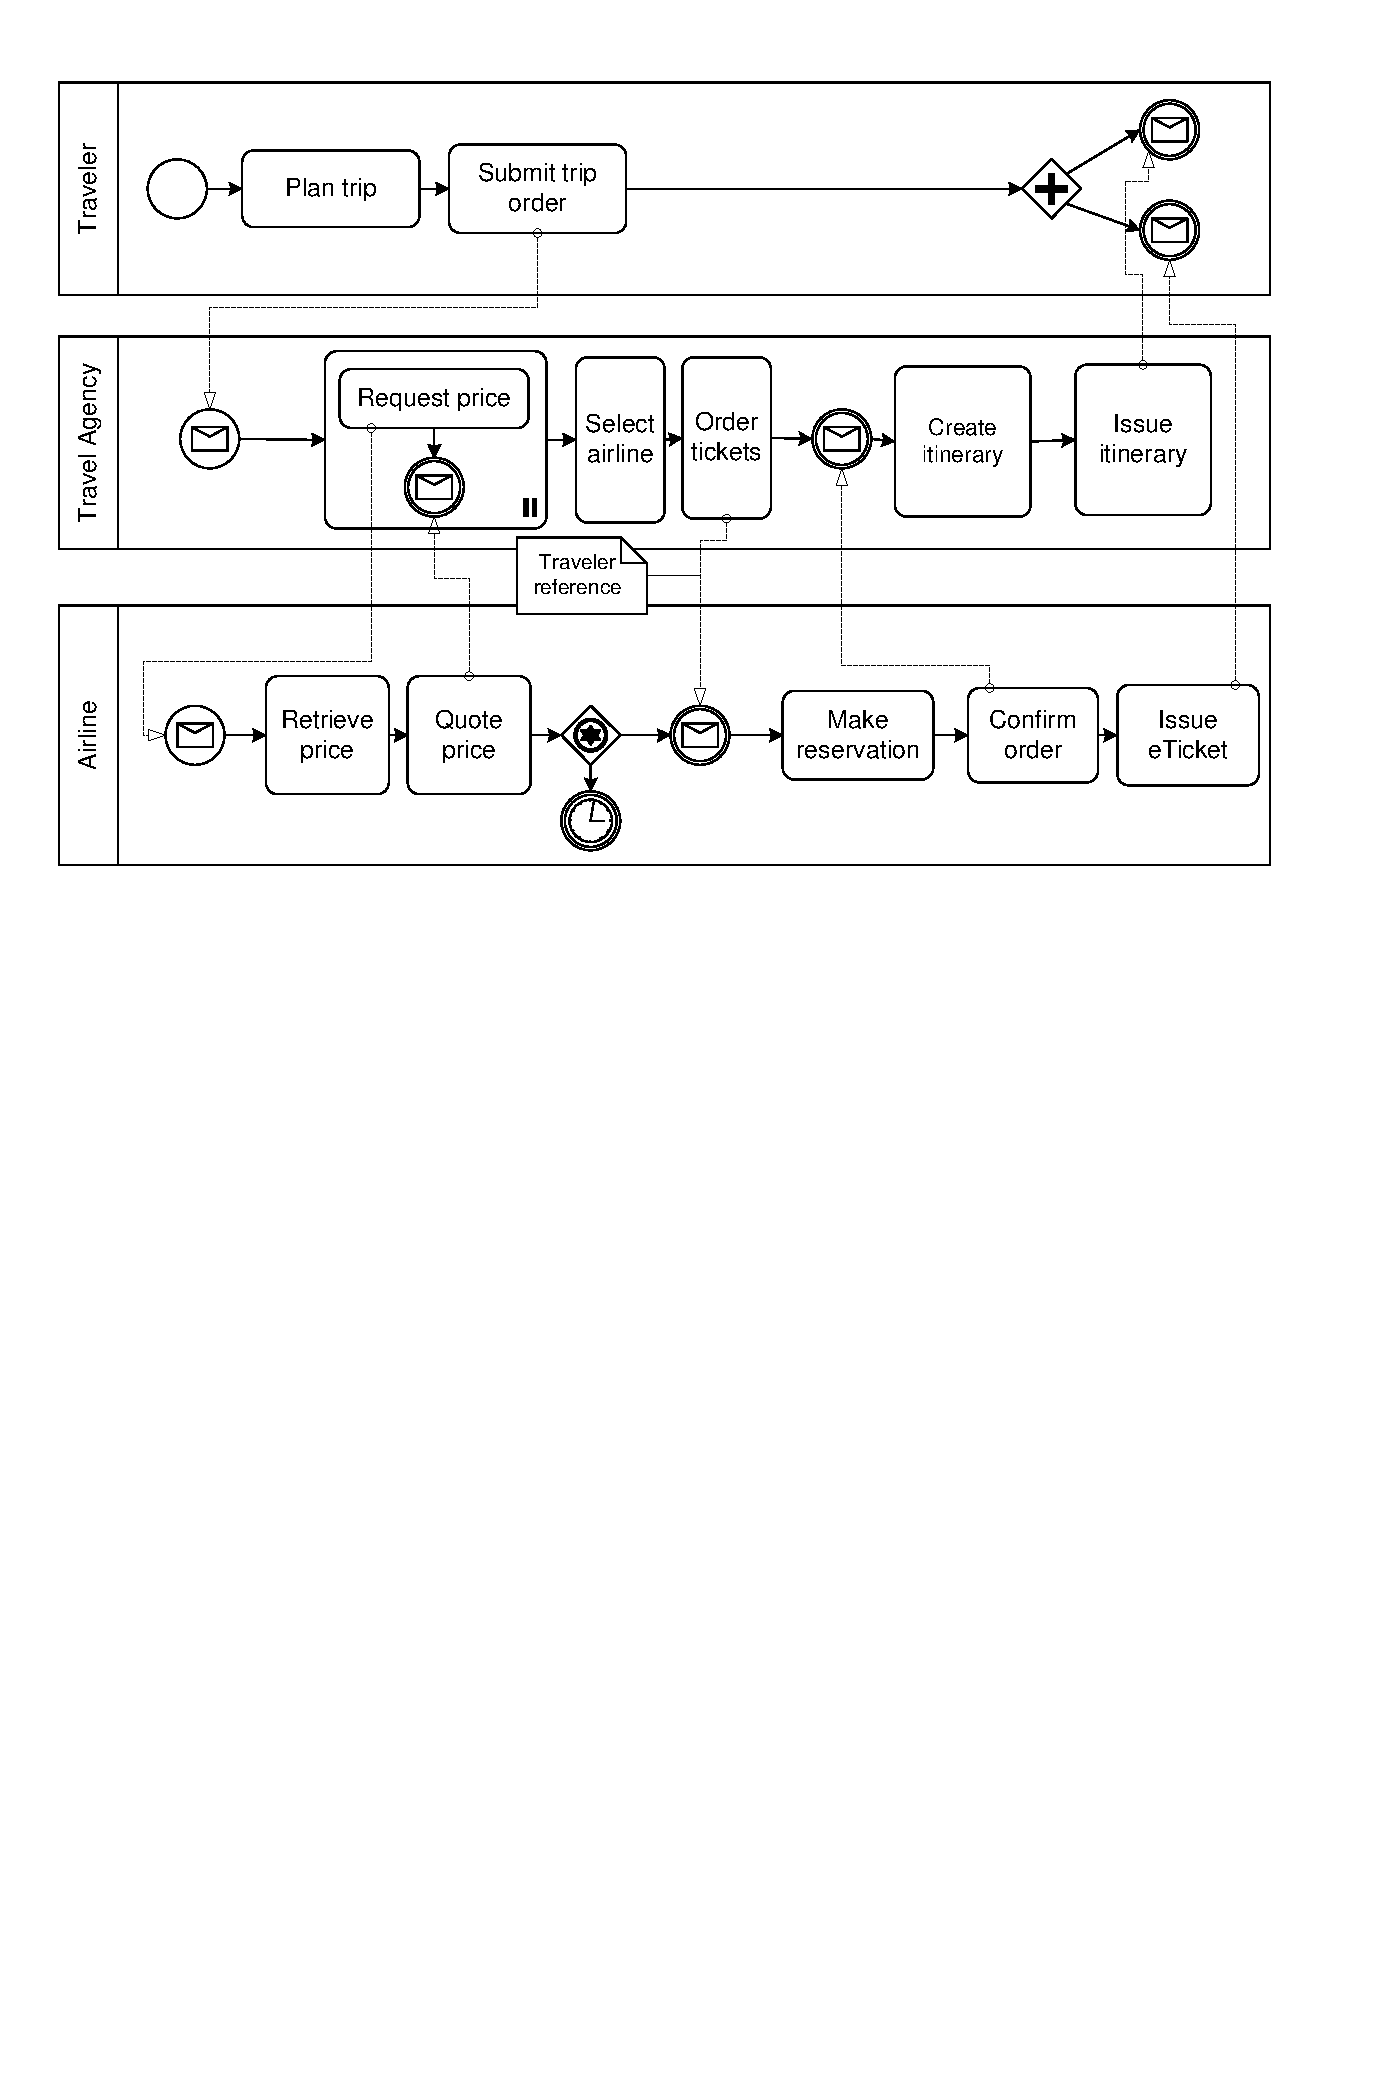
\includegraphics[width=\textwidth]{figures/choreography.pdf}
  \caption{Example Choreography}
  \label{fig:chor1}
\end{figure}

\begin{figure}
  \centering
  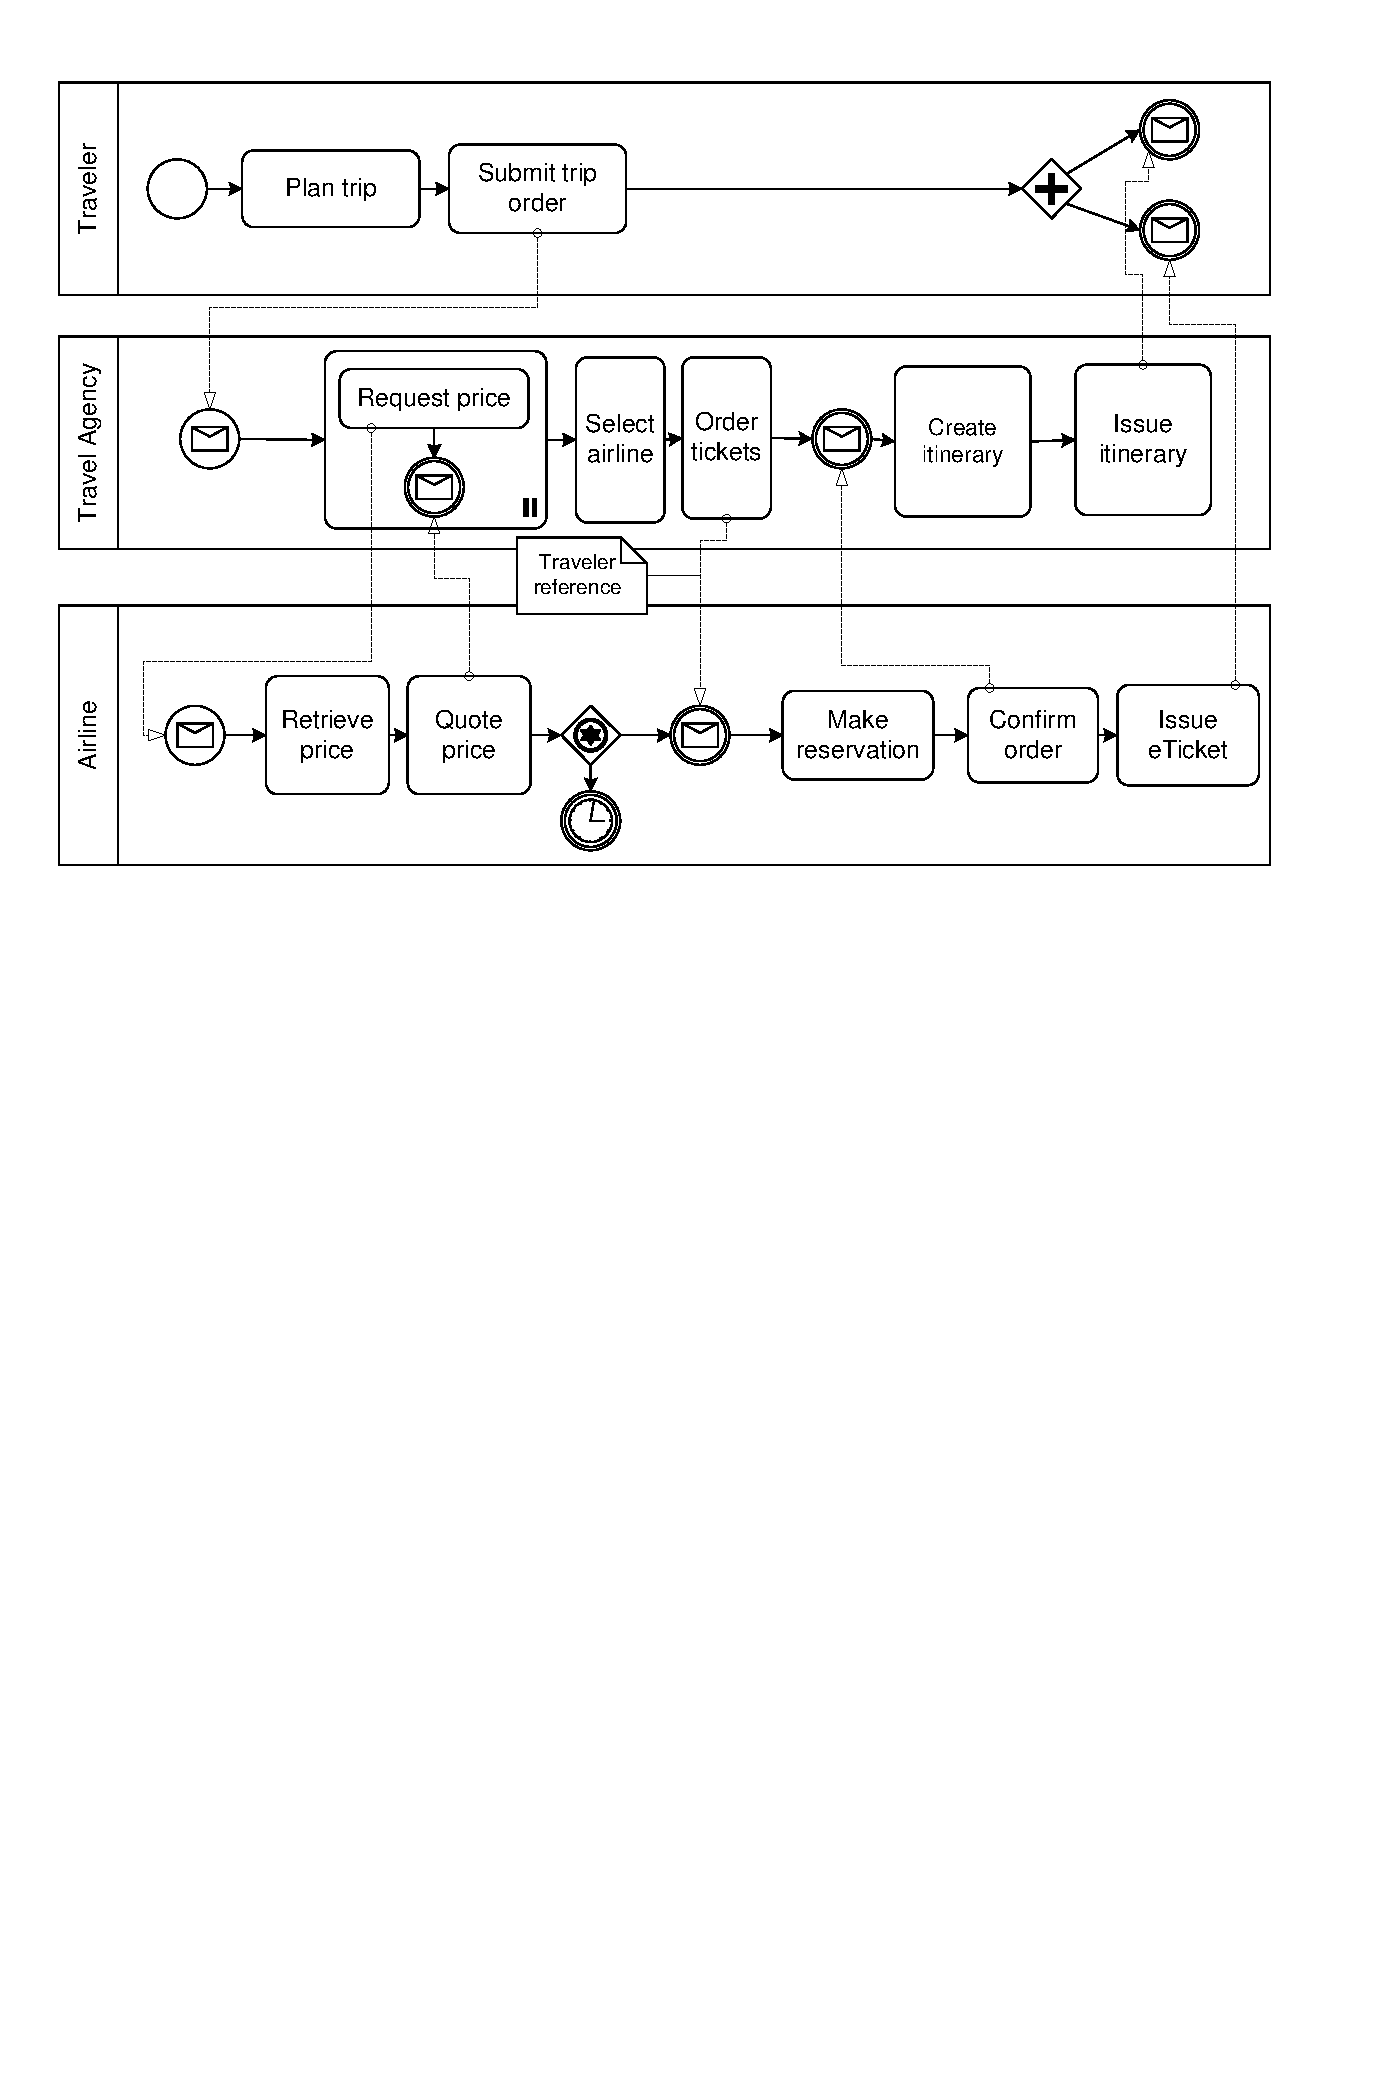
\includegraphics[width=.8\textwidth]{figures/choreography.pdf}
  \caption[Example Choreography]{The example choreography. Now slightly smaller to demonstrate \texttt{\textbackslash textwidth}. And also the use of alternative captions for the list of images. However, the latter is only conditionally recommended, because who reads so much text under a picture? Or is it just a matter of style?}
  \label{fig:chor2}
\end{figure}


\begin{figure}
  \hfill
  \begin{subfigure}{.3\textwidth}
    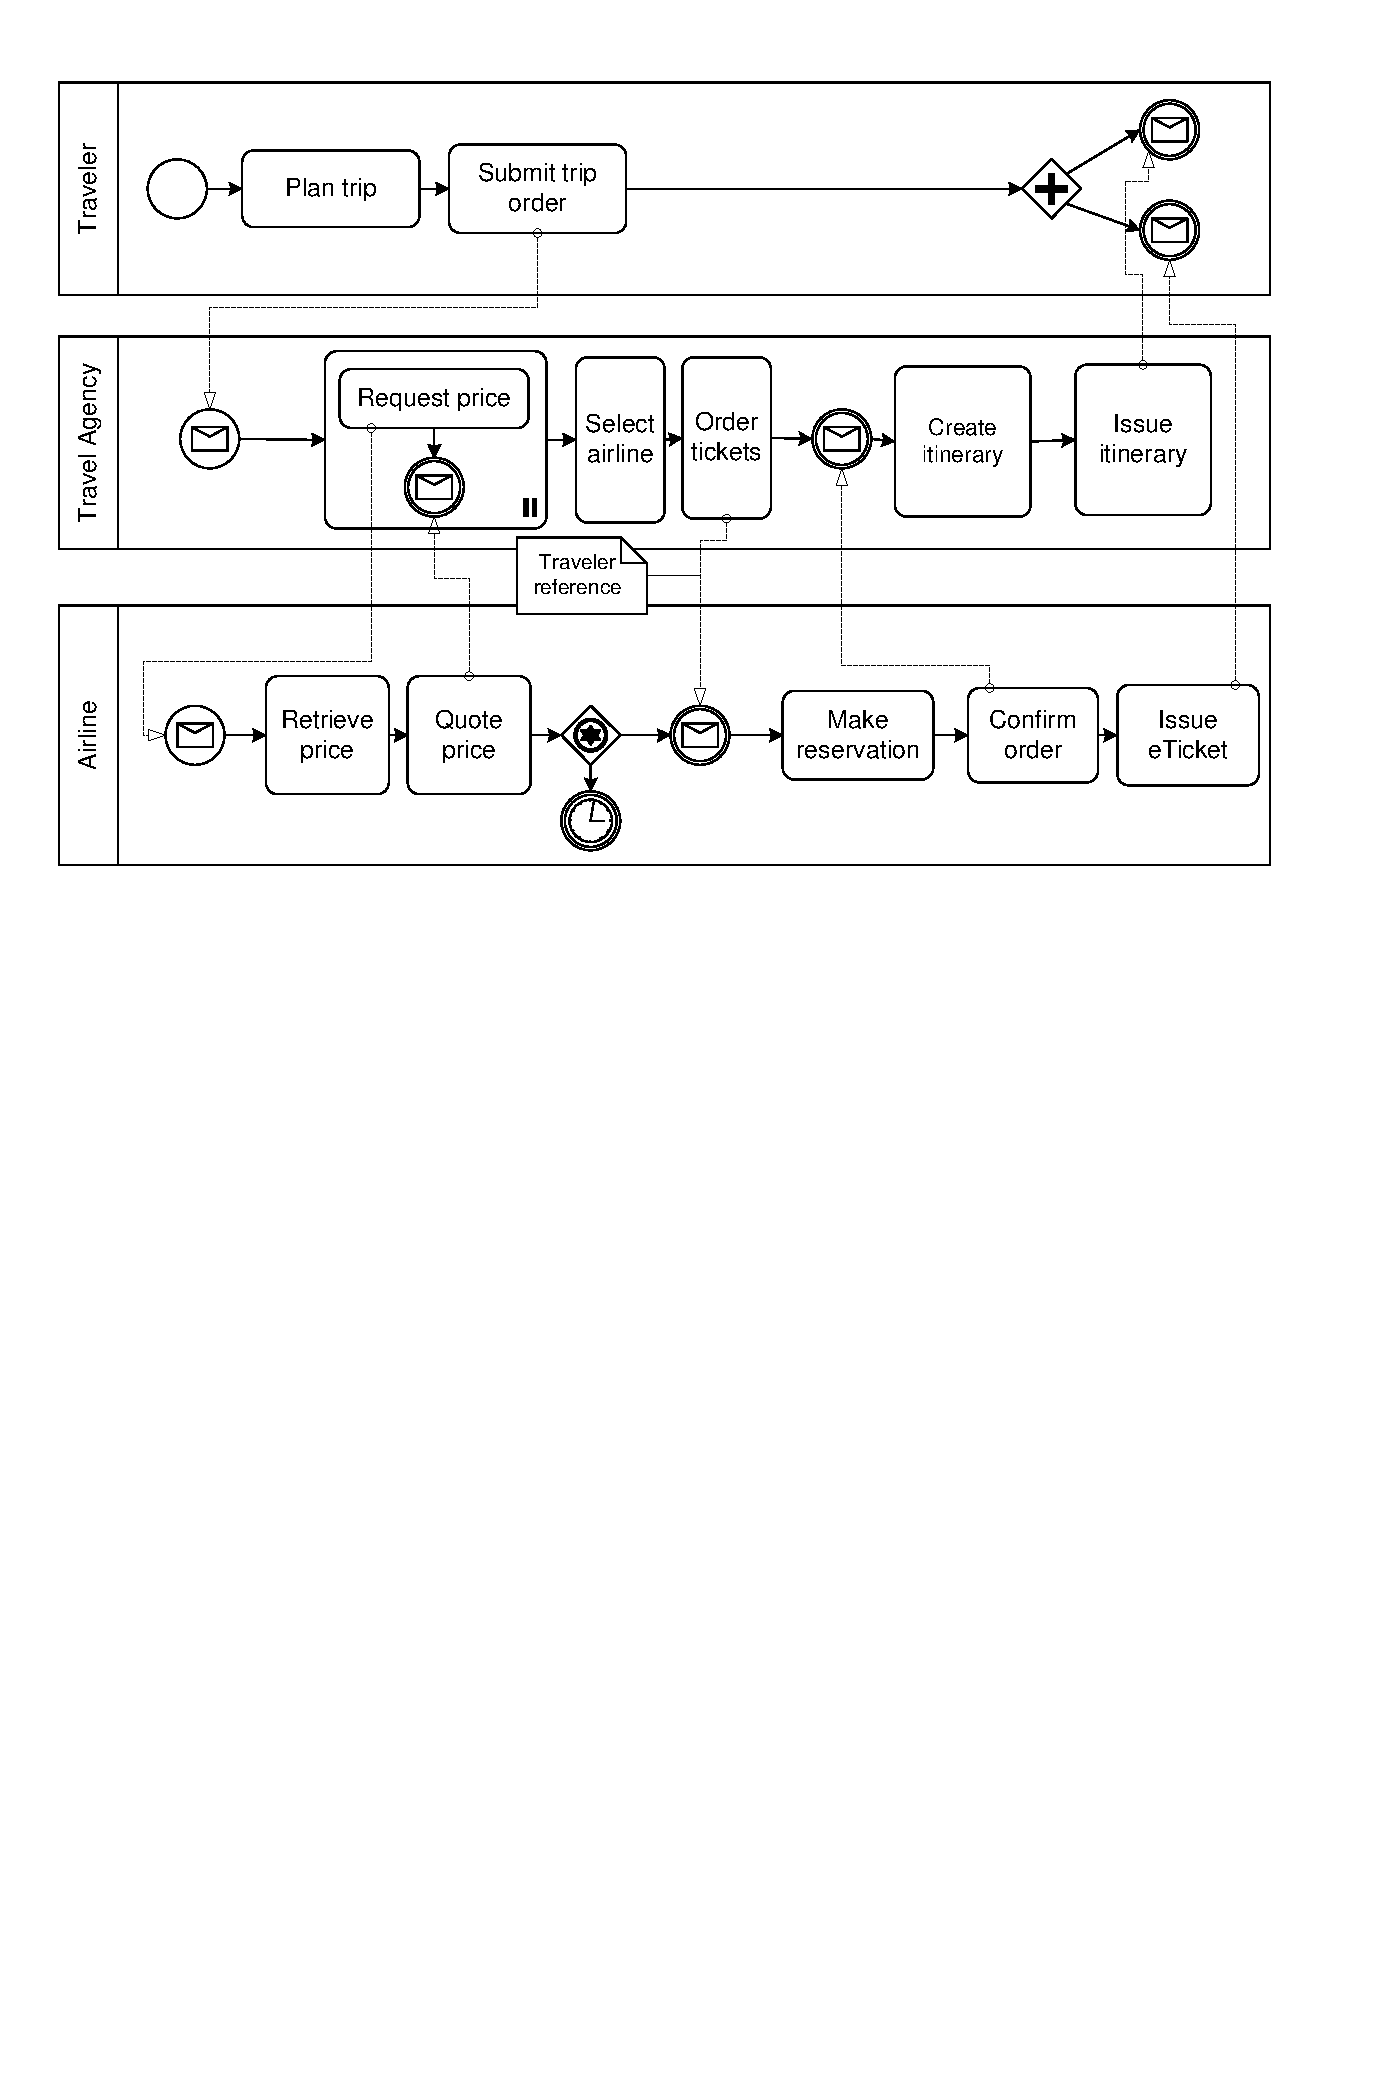
\includegraphics[width=\textwidth]{figures/choreography.pdf}
    \caption{Choreography 1}
    \label{fig:subfigA}
  \end{subfigure}
  \hfill
  \begin{subfigure}{.3\textwidth}
    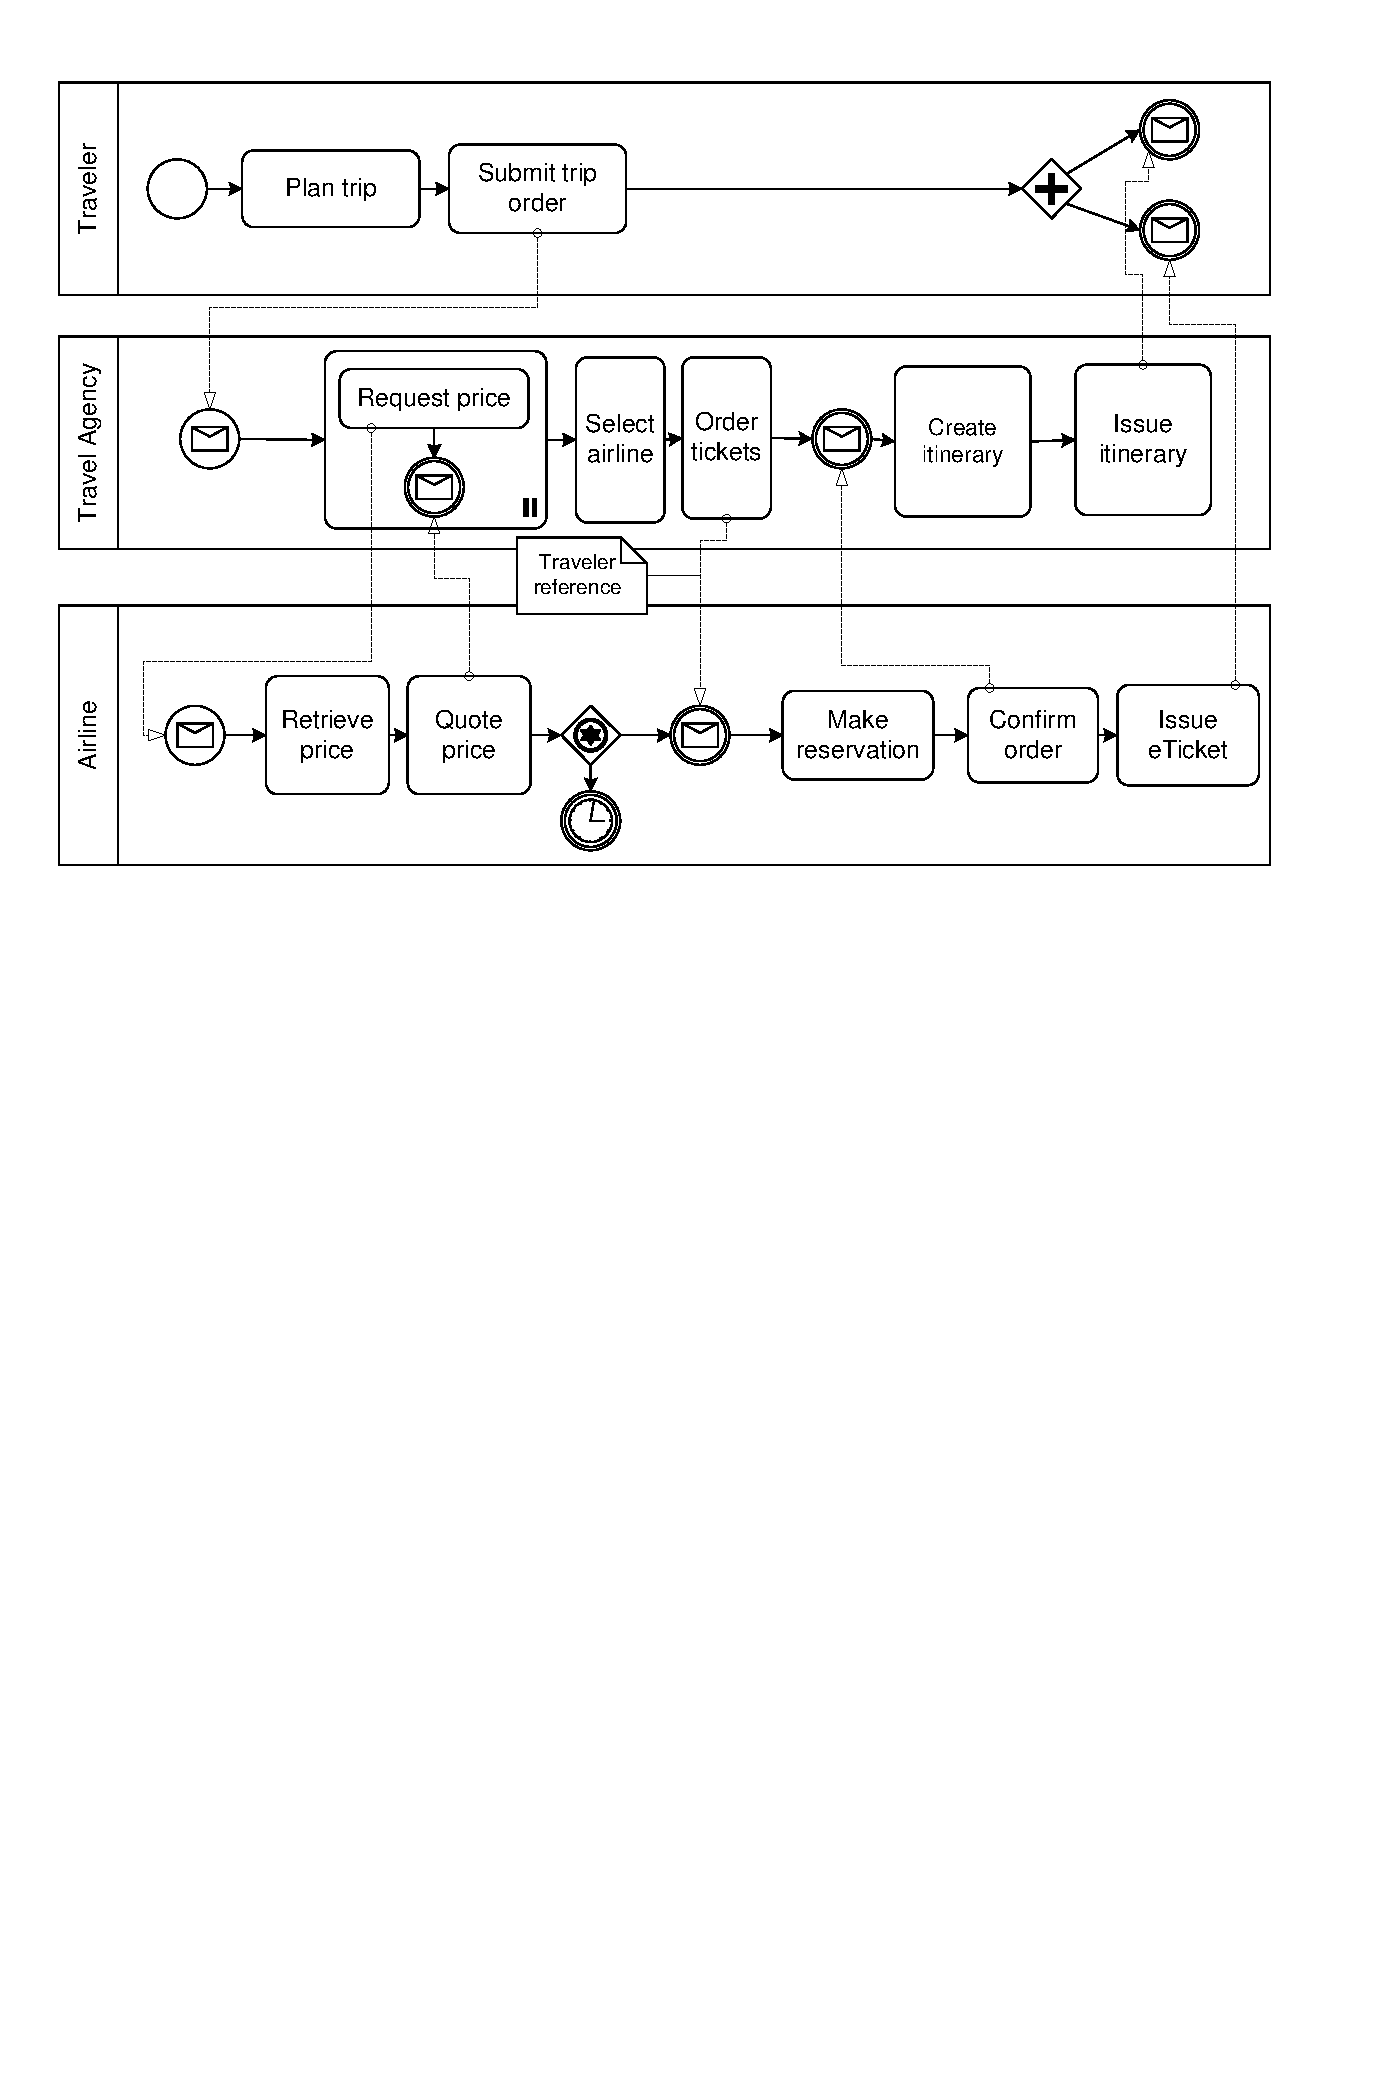
\includegraphics[width=\textwidth]{figures/choreography.pdf}
    \caption{Choreography 2}
    \label{fig:subfigB}
  \end{subfigure}
  \hfill
  \begin{subfigure}{.3\textwidth}
    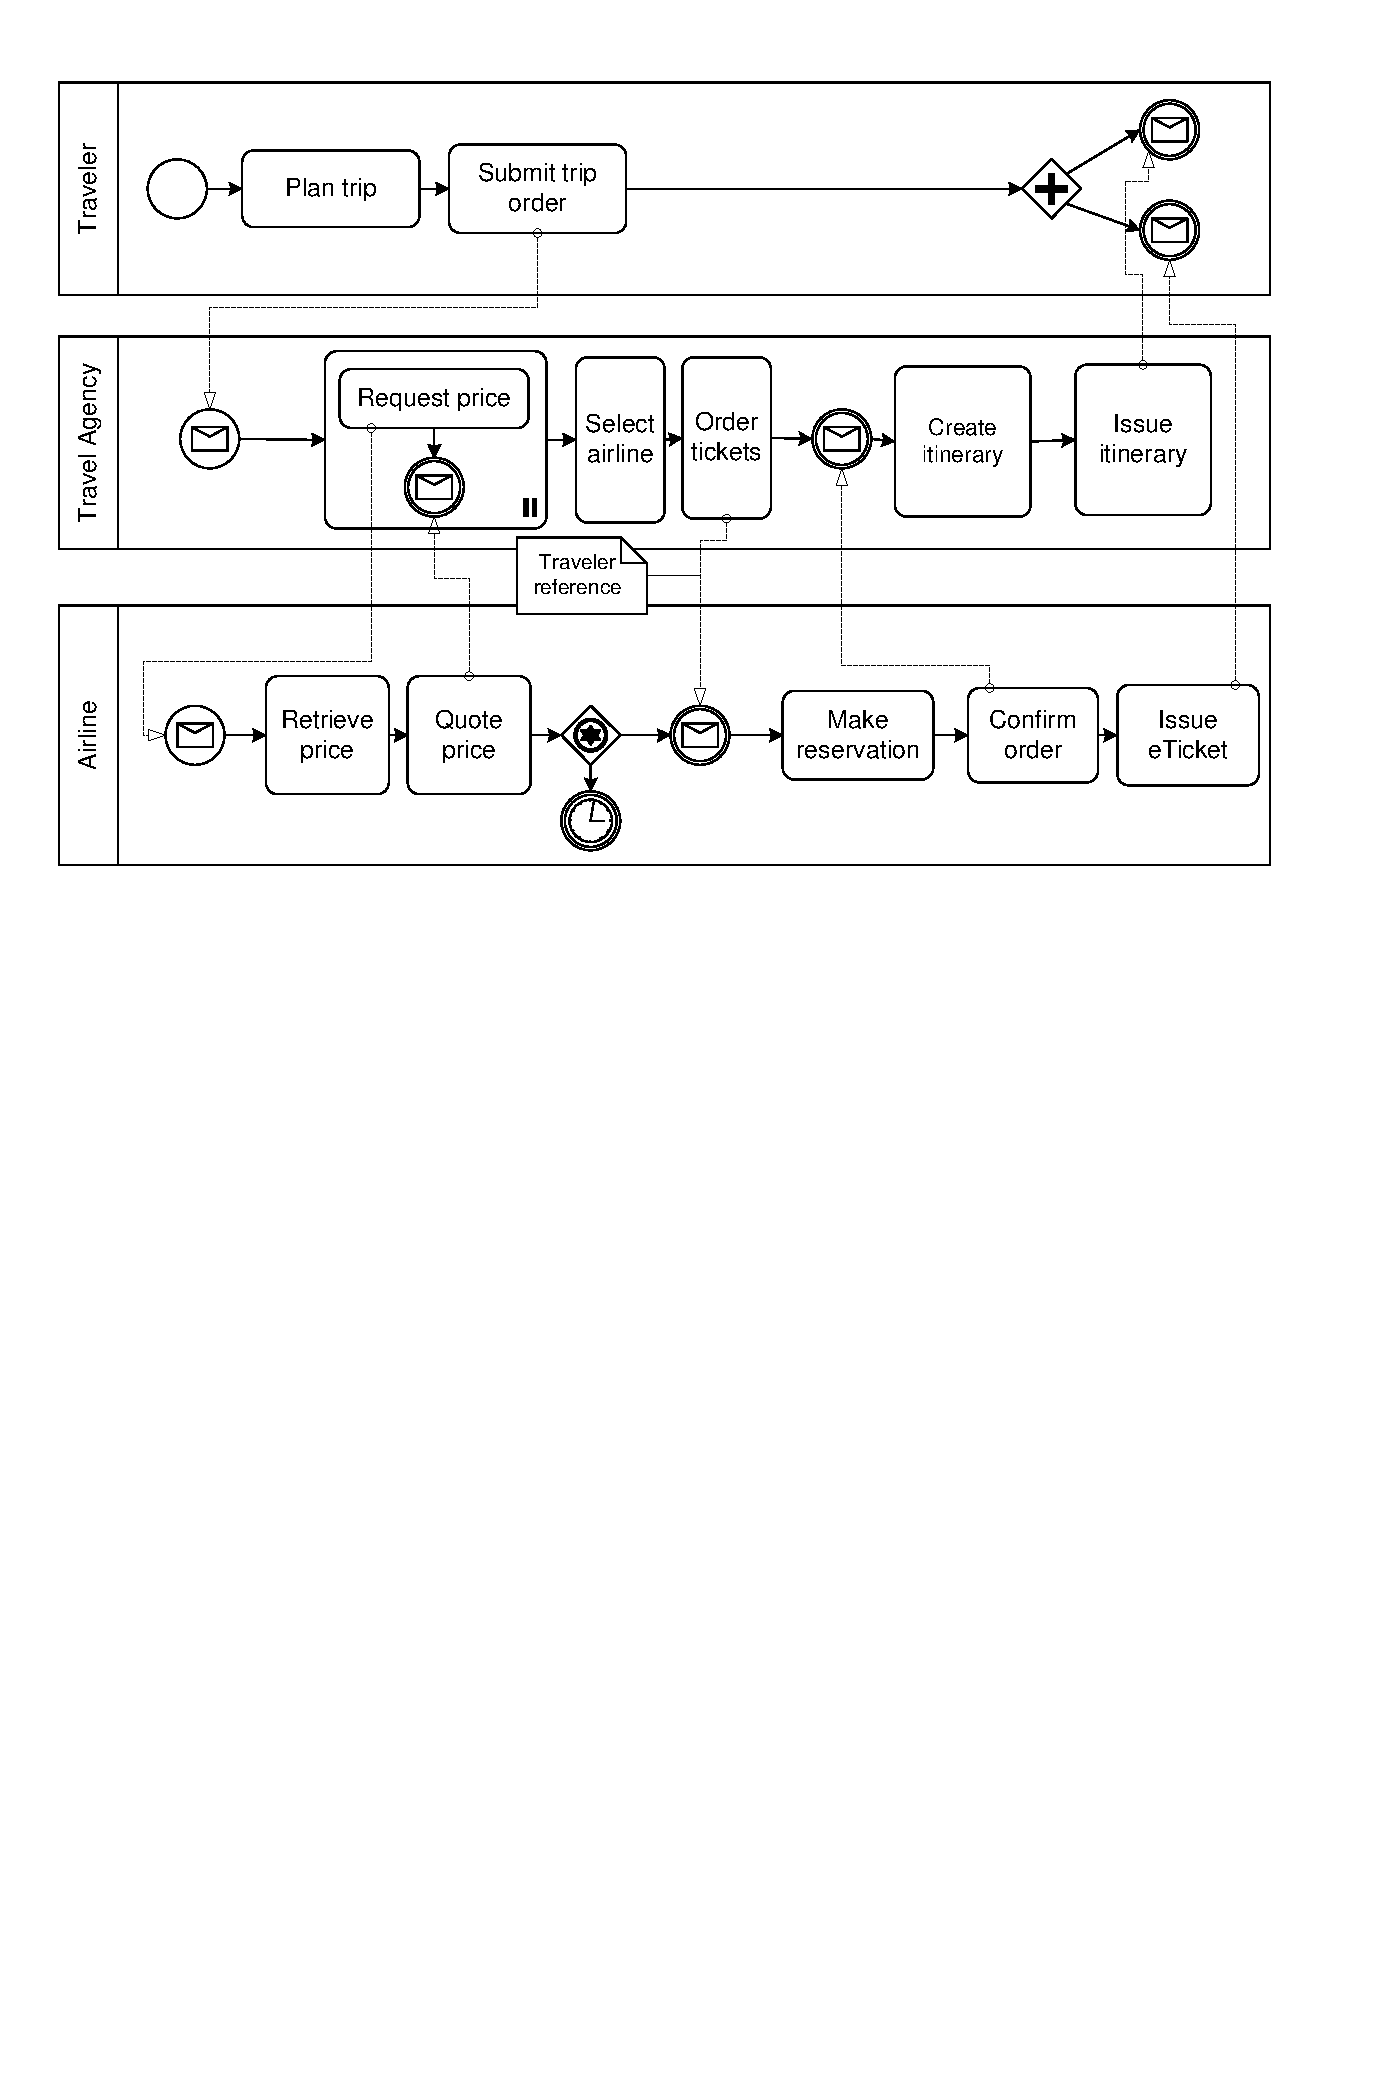
\includegraphics[width=.9\textwidth]{figures/choreography.pdf}
    \caption{Choreography 3}
    \label{fig:subfigC}
  \end{subfigure}
  \caption{Example to place 3 illustrations next to each other. Further, it is possible to reference each separately.}
  \label{fig:subfig_example}
\end{figure}

\autoref{fig:subfig_example} shows the usage of the package subcaption.
It is indeed possible to reference to sub figures: \autoref{fig:subfigA}.

It is possible to convert SVGs to PDF directly during compilation.
This is described in the source code of latex-tipps.tex, but commented out.

\iffalse % <-- Take this away if inkscape is in the path
  The SVG in \autoref{fig:directSVG} is directly included, while the text in the SVG in \autoref{fig:latexSVG} is set using pdflatex.
  If you want to see the graphics, inkscape must be in PATH and in the text source \texttt{\textbackslash{}iffalse} and \text{\textbackslash{}iftrue} have to be commented out.

  \begin{figure}
    \centering
    \includegraphics{svgexample.svg}
    \caption{SVG directly included}
    \label{fig:directSVG}
  \end{figure}

  \begin{figure}
    \centering
    \def\svgwidth{.4\textwidth}
    \includesvg{svgexample}
    \caption{Text in SVN set via \LaTeX{}}
    \label{fig:latexSVG}
  \end{figure}
\fi % <-- Take this away if inkscape is in the path



\section{More Illustrations}
\autoref{fig:AnhangsChor} and \ref{fig:AnhangsChor2} show two choreographies, which should further explain the facts. The second figure is rotated 90 degrees to demonstrate the \texttt{pdflscape} package.

\begin{figure}
  \centering
  \includegraphics[width=\textwidth]{figures/choreography.pdf}
  \caption{Example Choreography I}
  \label{fig:AnhangsChor}
\end{figure}

\begin{landscape}
  %sidewaysfigure
  \begin{figure}
    \centering
    \includegraphics[width=\textwidth]{figures/choreography.pdf}
    \caption{Example Choreography II}
    \label{fig:AnhangsChor2}
  \end{figure}
\end{landscape}


%\IfFileExists{pgfplots.sty}{
%  %%%%%%%%%%%%%%%%%%%%%%%%%%%%%%%%%%%%%%%%%%%%%%%%%%%%%%%%%%%%%%%%%%%%%%%%%%%%%%
%  \section{Plots with pgfplots}
%  %%%%%%%%%%%%%%%%%%%%%%%%%%%%%%%%%%%%%%%%%%%%%%%%%%%%%%%%%%%%%%%%%%%%%%%%%%%%%%
%  The package pdfplots provides plotting of functions directly in \LaTeX~like with matlab or gnuplot. Some visual examples are available here\footnote{\url{http://texdoc.net/pkg/visualtikz}}.
%  \begin{figure}[h]
%    \centering
%    \begin{tikzpicture}
%      \begin{axis}[xlabel=$x$,
%          ylabel=$\sin(x)$]
%        \addplot {sin(deg(x))};  % Print sine function
%      \end{axis}
%    \end{tikzpicture}
%    \caption{Plot of $\sin(x)$ direclty inside the figure environment with pgfplots.}
%  \end{figure}
%
%  \begin{figure}[h]
%    \centering
%    \begin{tikzpicture}
%      \begin{axis}[xlabel=$x$,
%          ylabel=$y$]
%        \addplot table [x=a, y=c, col sep=comma] {data/data.csv};  % Read coordinates from csv file and plot them
%      \end{axis}
%    \end{tikzpicture}
%    \caption{Coordinates $x$ and $y$ read from csv file and plotted pgfplots.}
%  \end{figure}
%
%}{}


% Note: Don't do this. Use Python or R for your figures.
%%%%%%%%%%%%%%%%%%%%%%%%%%%%%%%%%%%%%%%%%%%%%%%%%%%%%%%%%%%%%%%%%%%%%%%%%%%%%%%
%\section{Figures with tikz}
%%%%%%%%%%%%%%%%%%%%%%%%%%%%%%%%%%%%%%%%%%%%%%%%%%%%%%%%%%%%%%%%%%%%%%%%%%%%%%%


%%%%%%%%%%%%%%%%%%%%%%%%%%%%%%%%%%%%%%%%%%%%%%%%%%%%%%%%%%%%%%%%%%%%%%%%%%%%%%
\section{Linguistic Forests}
%%%%%%%%%%%%%%%%%%%%%%%%%%%%%%%%%%%%%%%%%%%%%%%%%%%%%%%%%%%%%%%%%%%%%%%%%%%%%%

\begin{filecontents*}{\democodefile}
\begin{forest}
  [VP
    [DP]
    [V’
      [V]
      [DP]
    ]
  ]
\end{forest}
\end{filecontents*}
\PrintDemo{style=parallel}


%%%%%%%%%%%%%%%%%%%%%%%%%%%%%%%%%%%%%%%%%%%%%%%%%%%%%%%%%%%%%%%%%%%%%%%%%%%%%%
\section{Tables}
%%%%%%%%%%%%%%%%%%%%%%%%%%%%%%%%%%%%%%%%%%%%%%%%%%%%%%%%%%%%%%%%%%%%%%%%%%%%%%
\autoref{tab:Ergebnisse} shows results and \autoref{tab:Werte} shows how numerical data can be represented in a table.
\begin{table}
  \centering
  \begin{tabular}{ccc}
    \toprule
    \multicolumn{2}{c}{\textbf{summed}} & \textbf{Title}                                                          \\ \midrule
    Table                                      & as                                                           & in      \\
    \url{tabsatz.pdf}                            & recommended                                                     & gesetzt \\

    \multirow{2}{*}{Example}                    & \multicolumn{2}{c}{a nice example}                                \\
                                                 & \multicolumn{2}{c}{for using \textit{multirow}}           \\
    \bottomrule
  \end{tabular}
  \caption[Example Table]{Exampe Table -- see \url{http://www.ctan.org/tex-archive/info/german/tabsatz/}}
  \label{tab:Ergebnisse}
\end{table}

\begin{table}
  \centering
  \begin{tabular}{l *{8}{d{3.2}}}
    \toprule

                         & \multicolumn{2}{c}{\textbf{Parameter 1}} & \multicolumn{2}{c}{\textbf{Parameter 2}} & \multicolumn{2}{c}{\textbf{Parameter 3}} & \multicolumn{2}{c}{\textbf{Parameter 4}}                                                                                                                                       \\
    \cmidrule(r){2-3}\cmidrule(lr){4-5}\cmidrule(lr){6-7}\cmidrule(l){8-9}

    \textbf{Bedingungen} & \multicolumn{1}{c}{\textbf{M}}           & \multicolumn{1}{c}{\textbf{SD}}          & \multicolumn{1}{c}{\textbf{M}}           & \multicolumn{1}{c}{\textbf{SD}}          & \multicolumn{1}{c}{\textbf{M}} & \multicolumn{1}{c}{\textbf{SD}} & \multicolumn{1}{c}{\textbf{M}} & \multicolumn{1}{c}{\textbf{SD}} \\
    \midrule

    W                    & 1.1                                      & 5.55                                     & 6.66                                     & .01                                      &                                &                                 &                                &                                 \\
    X                    & 22.22                                    & 0.0                                      & 77.5                                     & .1                                       &                                &                                 &                                &                                 \\
    Y                    & 333.3                                    & .1                                       & 11.11                                    & .05                                      &                                &                                 &                                &                                 \\
    Z                    & 4444.44                                  & 77.77                                    & 14.06                                    & .3                                       &                                &                                 &                                &                                 \\
    \bottomrule
  \end{tabular}

  \caption{Example table for 4 constraints (W-Z), each having 4 parameters with (M und SD). Note: use always the same number of decimal places.}
  \label{tab:Werte}
\end{table}

\section{Tables spanning multiple pages}


\begin{longtable}{lll}
\caption{A sample long table.} \label{tab:long} \\

\toprule \multicolumn{1}{c}{\textbf{First column}} & \multicolumn{1}{c}{\textbf{Second column}} & \multicolumn{1}{c}{\textbf{Third column}} \\ \midrule
\endfirsthead

\multicolumn{3}{c}%
{{\bfseries \tablename\ \thetable{} -- continued from previous page}} \\
\hline \multicolumn{1}{c}{\textbf{First column}} & \multicolumn{1}{c}{\textbf{Second column}} & \multicolumn{1}{c}{\textbf{Third column}} \\ \midrule
\endhead

\midrule \multicolumn{3}{r}{{Continued on next page}} \\ \midrule
\endfoot

\bottomrule
\endlastfoot

A & BC & D \\
A & BC & D \\
A & BC & D \\
A & BC & D \\

\end{longtable}


%%%%%%%%%%%%%%%%%%%%%%%%%%%%%%%%%%%%%%%%%%%%%%%%%%%%%%%%%%%%%%%%%%%%%%%%%%%%%%

%%%%%%%%%%%%%%%%%%%%%%%%%%%%%%%%%%%%%%%%%%%%%%%%%%%%%%%%%%%%%%%%%%%%%%%%%%%%%%


%With MiKTeX installation from 2012-01-16 no longer necessary.
%If a section becomes longer than one page and you want to refer to a specific place in the section with \texttt{\textbackslash{}vref}, then you should use \texttt{\textbackslash{}phantomsection} then using \texttt{vref} will also display the correct page number.

%%The link location will be placed on the line below.
%%Tipp von http://en.wikibooks.org/wiki/LaTeX/Labels_and_Cross-referencing#The_hyperref_package_and_.5Cphantomsection
%\phantomsection
%\label{alabel}
%View the example for \texttt{\textbackslash{}phantomsection} in the \LaTeX{} source code.

%Here is the example: See Section \vref{hack1} and Section \vref{hack2}.
%%%%%%%%%%%%%%%%%%%%%%%%%%%%%%%%%%%%%%%%%%%%%%%%%%%%%%%%%%%%%%%%%%%%%%%%%%%%%%
%\section{Definitions}
%%%%%%%%%%%%%%%%%%%%%%%%%%%%%%%%%%%%%%%%%%%%%%%%%%%%%%%%%%%%%%%%%%%%%%%%%%%%%%%
%\begin{definition}[Title]
%  \label{def:def1}
%  Definition Text
%\end{definition}
%
%\autoref{def:def1} shows \ldots

%%%%%%%%%%%%%%%%%%%%%%%%%%%%%%%%%%%%%%%%%%%%%%%%%%%%%%%%%%%%%%%%%%%%%%%%%%%%%%

%%%%%%%%%%%%%%%%%%%%%%%%%%%%%%%%%%%%%%%%%%%%%%%%%%%%%%%%%%%%%%%%%%%%%%%%%%%%%%

\pagestyle{empty}
\renewcommand*{\chapterpagestyle}{empty}
\Affirmation
%TC:endignore
\end{document}